\documentclass{book}
\usepackage[a4paper,top=2.5cm,bottom=2.5cm,left=2.5cm,right=2.5cm]{geometry}
\usepackage{makeidx}
\usepackage{natbib}
\usepackage{graphicx}
\usepackage{multicol}
\usepackage{float}
\usepackage{listings}
\usepackage{color}
\usepackage{ifthen}
\usepackage[table]{xcolor}
\usepackage{textcomp}
\usepackage{alltt}
\usepackage{ifpdf}
\ifpdf
\usepackage[pdftex,
            pagebackref=true,
            colorlinks=true,
            linkcolor=blue,
            unicode
           ]{hyperref}
\else
\usepackage[ps2pdf,
            pagebackref=true,
            colorlinks=true,
            linkcolor=blue,
            unicode
           ]{hyperref}
\usepackage{pspicture}
\fi
\usepackage[utf8]{inputenc}
\usepackage{mathptmx}
\usepackage[scaled=.90]{helvet}
\usepackage{courier}
\usepackage{sectsty}
\usepackage{amssymb}
\usepackage[titles]{tocloft}
\usepackage{doxygen}
\lstset{language=C++,inputencoding=utf8,basicstyle=\footnotesize,breaklines=true,breakatwhitespace=true,tabsize=4,numbers=left }
\makeindex
\setcounter{tocdepth}{3}
\renewcommand{\footrulewidth}{0.4pt}
\renewcommand{\familydefault}{\sfdefault}
\hfuzz=15pt
\setlength{\emergencystretch}{15pt}
\hbadness=750
\tolerance=750
\begin{document}
\hypersetup{pageanchor=false,citecolor=blue}
\begin{titlepage}
\vspace*{7cm}
\begin{center}
{\Large Fluid Survival Tool \\[1ex]\large 0.\-01 }\\
\vspace*{1cm}
{\large Generated by Doxygen 1.8.3.1}\\
\vspace*{0.5cm}
{\small Wed Apr 10 2013 11:10:04}\\
\end{center}
\end{titlepage}
\clearemptydoublepage
\pagenumbering{roman}
\tableofcontents
\clearemptydoublepage
\pagenumbering{arabic}
\hypersetup{pageanchor=true,citecolor=blue}
\chapter{Hierarchical Index}
\section{Class Hierarchy}
This inheritance list is sorted roughly, but not completely, alphabetically\-:\begin{DoxyCompactList}
\item \contentsline{section}{model\-:\-:Arc}{\pageref{structmodel_1_1Arc}}{}
\item \contentsline{section}{Clipper\-Lib\-:\-:Clipper\-Base}{\pageref{classClipperLib_1_1ClipperBase}}{}
\begin{DoxyCompactList}
\item \contentsline{section}{Clipper\-Lib\-:\-:Clipper}{\pageref{classClipperLib_1_1Clipper}}{}
\end{DoxyCompactList}
\item \contentsline{section}{Clipper\-Lib\-:\-:Double\-Point}{\pageref{structClipperLib_1_1DoublePoint}}{}
\item \contentsline{section}{model\-:\-:Dtrm\-Event}{\pageref{structmodel_1_1DtrmEvent}}{}
\item exception\begin{DoxyCompactList}
\item \contentsline{section}{Clipper\-Lib\-:\-:clipper\-Exception}{\pageref{classClipperLib_1_1clipperException}}{}
\end{DoxyCompactList}
\item \contentsline{section}{model\-:\-:Facade}{\pageref{classmodel_1_1Facade}}{}
\item \contentsline{section}{model\-:\-:Formula}{\pageref{classmodel_1_1Formula}}{}
\begin{DoxyCompactList}
\item \contentsline{section}{model\-:\-:A\-D\-Formula}{\pageref{classmodel_1_1ADFormula}}{}
\item \contentsline{section}{model\-:\-:A\-D\-Formula}{\pageref{classmodel_1_1ADFormula}}{}
\item \contentsline{section}{model\-:\-:And\-Formula}{\pageref{classmodel_1_1AndFormula}}{}
\item \contentsline{section}{model\-:\-:And\-Formula}{\pageref{classmodel_1_1AndFormula}}{}
\item \contentsline{section}{model\-:\-:Atom\-Cont\-Formula}{\pageref{classmodel_1_1AtomContFormula}}{}
\item \contentsline{section}{model\-:\-:Atom\-Cont\-Formula}{\pageref{classmodel_1_1AtomContFormula}}{}
\item \contentsline{section}{model\-:\-:Atom\-Dis\-Formula}{\pageref{classmodel_1_1AtomDisFormula}}{}
\item \contentsline{section}{model\-:\-:Atom\-Dis\-Formula}{\pageref{classmodel_1_1AtomDisFormula}}{}
\item \contentsline{section}{model\-:\-:Neg\-Formula}{\pageref{classmodel_1_1NegFormula}}{}
\item \contentsline{section}{model\-:\-:Neg\-Formula}{\pageref{classmodel_1_1NegFormula}}{}
\item \contentsline{section}{model\-:\-:Prob\-Formula}{\pageref{classmodel_1_1ProbFormula}}{}
\item \contentsline{section}{model\-:\-:Prob\-Formula}{\pageref{classmodel_1_1ProbFormula}}{}
\item \contentsline{section}{model\-:\-:True\-Formula}{\pageref{classmodel_1_1TrueFormula}}{}
\item \contentsline{section}{model\-:\-:True\-Formula}{\pageref{classmodel_1_1TrueFormula}}{}
\item \contentsline{section}{model\-:\-:Until\-Formula}{\pageref{classmodel_1_1UntilFormula}}{}
\item \contentsline{section}{model\-:\-:Until\-Formula}{\pageref{classmodel_1_1UntilFormula}}{}
\end{DoxyCompactList}
\item \contentsline{section}{Formula}{\pageref{structFormula}}{}
\item \contentsline{section}{model\-:\-:Geometry\-Helper}{\pageref{classmodel_1_1GeometryHelper}}{}
\item \contentsline{section}{Clipper\-Lib\-:\-:Horz\-Join\-Rec}{\pageref{structClipperLib_1_1HorzJoinRec}}{}
\item \contentsline{section}{Clipper\-Lib\-:\-:Int128}{\pageref{classClipperLib_1_1Int128}}{}
\item \contentsline{section}{Clipper\-Lib\-:\-:Intersect\-Node}{\pageref{structClipperLib_1_1IntersectNode}}{}
\item \contentsline{section}{Interval}{\pageref{structInterval}}{}
\item \contentsline{section}{model\-:\-:Interval}{\pageref{classmodel_1_1Interval}}{}
\item \contentsline{section}{model\-:\-:Interval\-Set}{\pageref{classmodel_1_1IntervalSet}}{}
\item \contentsline{section}{Clipper\-Lib\-:\-:Int\-Point}{\pageref{structClipperLib_1_1IntPoint}}{}
\item \contentsline{section}{Clipper\-Lib\-:\-:Int\-Rect}{\pageref{structClipperLib_1_1IntRect}}{}
\item \contentsline{section}{Clipper\-Lib\-:\-:Join\-Rec}{\pageref{structClipperLib_1_1JoinRec}}{}
\item \contentsline{section}{model\-:\-:Line}{\pageref{classmodel_1_1Line}}{}
\begin{DoxyCompactList}
\item \contentsline{section}{model\-:\-:Segment}{\pageref{classmodel_1_1Segment}}{}
\end{DoxyCompactList}
\item \contentsline{section}{Clipper\-Lib\-:\-:Local\-Minima}{\pageref{structClipperLib_1_1LocalMinima}}{}
\item \contentsline{section}{model\-:\-:location}{\pageref{classmodel_1_1location}}{}
\item \contentsline{section}{model\-:\-:Logger}{\pageref{classmodel_1_1Logger}}{}
\begin{DoxyCompactList}
\item \contentsline{section}{G\-U\-I\-Controller}{\pageref{classGUIController}}{}
\end{DoxyCompactList}
\item \contentsline{section}{model\-:\-:Marking}{\pageref{structmodel_1_1Marking}}{}
\item \contentsline{section}{model\-:\-:min\-List}{\pageref{structmodel_1_1minList}}{}
\item \contentsline{section}{model\-:\-:Model}{\pageref{structmodel_1_1Model}}{}
\item \contentsline{section}{model\-:\-:Model\-Checker}{\pageref{classmodel_1_1ModelChecker}}{}
\item \contentsline{section}{Clipper\-Lib\-:\-:Out\-Pt}{\pageref{structClipperLib_1_1OutPt}}{}
\item \contentsline{section}{Clipper\-Lib\-:\-:Out\-Rec}{\pageref{structClipperLib_1_1OutRec}}{}
\item \contentsline{section}{model\-:\-:Place}{\pageref{structmodel_1_1Place}}{}
\item \contentsline{section}{model\-:\-:Point}{\pageref{structmodel_1_1Point}}{}
\item \contentsline{section}{model\-:\-:Polygon}{\pageref{classmodel_1_1Polygon}}{}
\item \contentsline{section}{Clipper\-Lib\-:\-:Poly\-Node}{\pageref{classClipperLib_1_1PolyNode}}{}
\begin{DoxyCompactList}
\item \contentsline{section}{Clipper\-Lib\-:\-:Poly\-Tree}{\pageref{classClipperLib_1_1PolyTree}}{}
\end{DoxyCompactList}
\item \contentsline{section}{Clipper\-Lib\-:\-:Poly\-Offset\-Builder}{\pageref{classClipperLib_1_1PolyOffsetBuilder}}{}
\item \contentsline{section}{model\-:\-:position}{\pageref{classmodel_1_1position}}{}
\item Q\-Dialog\begin{DoxyCompactList}
\item \contentsline{section}{Model\-Check\-Dialog\-Controller}{\pageref{classModelCheckDialogController}}{}
\item \contentsline{section}{Place\-Prob\-Dialog\-Controller}{\pageref{classPlaceProbDialogController}}{}
\item \contentsline{section}{S\-T\-D\-Dialog\-Controller}{\pageref{classSTDDialogController}}{}
\end{DoxyCompactList}
\item Q\-Main\-Window\begin{DoxyCompactList}
\item \contentsline{section}{G\-U\-I\-Controller}{\pageref{classGUIController}}{}
\item \contentsline{section}{G\-U\-I\-Controller}{\pageref{classGUIController}}{}
\end{DoxyCompactList}
\item \contentsline{section}{model\-:\-:Region}{\pageref{classmodel_1_1Region}}{}
\item \contentsline{section}{Clipper\-Lib\-:\-:Scanbeam}{\pageref{structClipperLib_1_1Scanbeam}}{}
\item \contentsline{section}{model\-:\-:slice$<$ T, S $>$}{\pageref{classmodel_1_1slice}}{}
\item \contentsline{section}{model\-:\-:stack$<$ T, S $>$}{\pageref{classmodel_1_1stack}}{}
\item \contentsline{section}{model\-:\-:State\-\_\-tag}{\pageref{structmodel_1_1State__tag}}{}
\item \contentsline{section}{model\-:\-:State\-Prob\-Alt\-\_\-tag}{\pageref{structmodel_1_1StateProbAlt__tag}}{}
\item \contentsline{section}{model\-:\-:State\-Time\-Alt\-\_\-tag}{\pageref{structmodel_1_1StateTimeAlt__tag}}{}
\item \contentsline{section}{model\-:\-:Stochastic\-Event}{\pageref{structmodel_1_1StochasticEvent}}{}
\item \contentsline{section}{Clipper\-Lib\-:\-:T\-Edge}{\pageref{structClipperLib_1_1TEdge}}{}
\item \contentsline{section}{model\-:\-:Timed\-Diagram}{\pageref{classmodel_1_1TimedDiagram}}{}
\item \contentsline{section}{Token}{\pageref{structToken}}{}
\item \contentsline{section}{model\-:\-:Transition}{\pageref{structmodel_1_1Transition}}{}
\item \contentsline{section}{yy\-\_\-buffer\-\_\-state}{\pageref{structyy__buffer__state}}{}
\item \contentsline{section}{yy\-\_\-trans\-\_\-info}{\pageref{structyy__trans__info}}{}
\item \contentsline{section}{yyalloc}{\pageref{unionyyalloc}}{}
\item \contentsline{section}{Y\-Y\-M\-I\-N\-O\-R\-T\-Y\-P\-E}{\pageref{unionYYMINORTYPE}}{}
\item \contentsline{section}{yy\-Parser}{\pageref{structyyParser}}{}
\item \contentsline{section}{yy\-Stack\-Entry}{\pageref{structyyStackEntry}}{}
\item \contentsline{section}{Y\-Y\-S\-T\-Y\-P\-E}{\pageref{unionYYSTYPE}}{}
\item \contentsline{section}{yystype}{\pageref{unionyystype}}{}
\end{DoxyCompactList}

\chapter{Class Index}
\section{Class List}
Here are the classes, structs, unions and interfaces with brief descriptions\-:\begin{DoxyCompactList}
\item\contentsline{section}{\hyperlink{classmodel_1_1ADFormula}{model\-::\-A\-D\-Formula} }{\pageref{classmodel_1_1ADFormula}}{}
\item\contentsline{section}{\hyperlink{classmodel_1_1AndFormula}{model\-::\-And\-Formula} }{\pageref{classmodel_1_1AndFormula}}{}
\item\contentsline{section}{\hyperlink{structmodel_1_1Arc}{model\-::\-Arc} }{\pageref{structmodel_1_1Arc}}{}
\item\contentsline{section}{\hyperlink{classmodel_1_1AtomContFormula}{model\-::\-Atom\-Cont\-Formula} }{\pageref{classmodel_1_1AtomContFormula}}{}
\item\contentsline{section}{\hyperlink{classmodel_1_1AtomDisFormula}{model\-::\-Atom\-Dis\-Formula} }{\pageref{classmodel_1_1AtomDisFormula}}{}
\item\contentsline{section}{\hyperlink{classClipperLib_1_1Clipper}{Clipper\-Lib\-::\-Clipper} }{\pageref{classClipperLib_1_1Clipper}}{}
\item\contentsline{section}{\hyperlink{classClipperLib_1_1ClipperBase}{Clipper\-Lib\-::\-Clipper\-Base} }{\pageref{classClipperLib_1_1ClipperBase}}{}
\item\contentsline{section}{\hyperlink{classClipperLib_1_1clipperException}{Clipper\-Lib\-::clipper\-Exception} }{\pageref{classClipperLib_1_1clipperException}}{}
\item\contentsline{section}{\hyperlink{structClipperLib_1_1DoublePoint}{Clipper\-Lib\-::\-Double\-Point} }{\pageref{structClipperLib_1_1DoublePoint}}{}
\item\contentsline{section}{\hyperlink{structmodel_1_1DtrmEvent}{model\-::\-Dtrm\-Event} }{\pageref{structmodel_1_1DtrmEvent}}{}
\item\contentsline{section}{\hyperlink{classmodel_1_1Facade}{model\-::\-Facade} }{\pageref{classmodel_1_1Facade}}{}
\item\contentsline{section}{\hyperlink{classmodel_1_1Formula}{model\-::\-Formula} }{\pageref{classmodel_1_1Formula}}{}
\item\contentsline{section}{\hyperlink{structFormula}{Formula} }{\pageref{structFormula}}{}
\item\contentsline{section}{\hyperlink{classmodel_1_1GeometryHelper}{model\-::\-Geometry\-Helper} }{\pageref{classmodel_1_1GeometryHelper}}{}
\item\contentsline{section}{\hyperlink{classGUIController}{G\-U\-I\-Controller} }{\pageref{classGUIController}}{}
\item\contentsline{section}{\hyperlink{structClipperLib_1_1HorzJoinRec}{Clipper\-Lib\-::\-Horz\-Join\-Rec} }{\pageref{structClipperLib_1_1HorzJoinRec}}{}
\item\contentsline{section}{\hyperlink{classClipperLib_1_1Int128}{Clipper\-Lib\-::\-Int128} }{\pageref{classClipperLib_1_1Int128}}{}
\item\contentsline{section}{\hyperlink{structClipperLib_1_1IntersectNode}{Clipper\-Lib\-::\-Intersect\-Node} }{\pageref{structClipperLib_1_1IntersectNode}}{}
\item\contentsline{section}{\hyperlink{structInterval}{Interval} }{\pageref{structInterval}}{}
\item\contentsline{section}{\hyperlink{classmodel_1_1Interval}{model\-::\-Interval} }{\pageref{classmodel_1_1Interval}}{}
\item\contentsline{section}{\hyperlink{classmodel_1_1IntervalSet}{model\-::\-Interval\-Set} }{\pageref{classmodel_1_1IntervalSet}}{}
\item\contentsline{section}{\hyperlink{structClipperLib_1_1IntPoint}{Clipper\-Lib\-::\-Int\-Point} }{\pageref{structClipperLib_1_1IntPoint}}{}
\item\contentsline{section}{\hyperlink{structClipperLib_1_1IntRect}{Clipper\-Lib\-::\-Int\-Rect} }{\pageref{structClipperLib_1_1IntRect}}{}
\item\contentsline{section}{\hyperlink{structClipperLib_1_1JoinRec}{Clipper\-Lib\-::\-Join\-Rec} }{\pageref{structClipperLib_1_1JoinRec}}{}
\item\contentsline{section}{\hyperlink{classmodel_1_1Line}{model\-::\-Line} }{\pageref{classmodel_1_1Line}}{}
\item\contentsline{section}{\hyperlink{structClipperLib_1_1LocalMinima}{Clipper\-Lib\-::\-Local\-Minima} }{\pageref{structClipperLib_1_1LocalMinima}}{}
\item\contentsline{section}{\hyperlink{classmodel_1_1location}{model\-::location} \\*Abstract a location }{\pageref{classmodel_1_1location}}{}
\item\contentsline{section}{\hyperlink{classmodel_1_1Logger}{model\-::\-Logger} }{\pageref{classmodel_1_1Logger}}{}
\item\contentsline{section}{\hyperlink{structmodel_1_1Marking}{model\-::\-Marking} }{\pageref{structmodel_1_1Marking}}{}
\item\contentsline{section}{\hyperlink{structmodel_1_1minList}{model\-::min\-List} }{\pageref{structmodel_1_1minList}}{}
\item\contentsline{section}{\hyperlink{structmodel_1_1Model}{model\-::\-Model} }{\pageref{structmodel_1_1Model}}{}
\item\contentsline{section}{\hyperlink{classModelCheckDialogController}{Model\-Check\-Dialog\-Controller} }{\pageref{classModelCheckDialogController}}{}
\item\contentsline{section}{\hyperlink{classmodel_1_1ModelChecker}{model\-::\-Model\-Checker} }{\pageref{classmodel_1_1ModelChecker}}{}
\item\contentsline{section}{\hyperlink{classmodel_1_1NegFormula}{model\-::\-Neg\-Formula} }{\pageref{classmodel_1_1NegFormula}}{}
\item\contentsline{section}{\hyperlink{structClipperLib_1_1OutPt}{Clipper\-Lib\-::\-Out\-Pt} }{\pageref{structClipperLib_1_1OutPt}}{}
\item\contentsline{section}{\hyperlink{structClipperLib_1_1OutRec}{Clipper\-Lib\-::\-Out\-Rec} }{\pageref{structClipperLib_1_1OutRec}}{}
\item\contentsline{section}{\hyperlink{structmodel_1_1Place}{model\-::\-Place} }{\pageref{structmodel_1_1Place}}{}
\item\contentsline{section}{\hyperlink{classPlaceProbDialogController}{Place\-Prob\-Dialog\-Controller} }{\pageref{classPlaceProbDialogController}}{}
\item\contentsline{section}{\hyperlink{structmodel_1_1Point}{model\-::\-Point} }{\pageref{structmodel_1_1Point}}{}
\item\contentsline{section}{\hyperlink{classmodel_1_1Polygon}{model\-::\-Polygon} }{\pageref{classmodel_1_1Polygon}}{}
\item\contentsline{section}{\hyperlink{classClipperLib_1_1PolyNode}{Clipper\-Lib\-::\-Poly\-Node} }{\pageref{classClipperLib_1_1PolyNode}}{}
\item\contentsline{section}{\hyperlink{classClipperLib_1_1PolyOffsetBuilder}{Clipper\-Lib\-::\-Poly\-Offset\-Builder} }{\pageref{classClipperLib_1_1PolyOffsetBuilder}}{}
\item\contentsline{section}{\hyperlink{classClipperLib_1_1PolyTree}{Clipper\-Lib\-::\-Poly\-Tree} }{\pageref{classClipperLib_1_1PolyTree}}{}
\item\contentsline{section}{\hyperlink{classmodel_1_1position}{model\-::position} \\*Abstract a position }{\pageref{classmodel_1_1position}}{}
\item\contentsline{section}{\hyperlink{classmodel_1_1ProbFormula}{model\-::\-Prob\-Formula} }{\pageref{classmodel_1_1ProbFormula}}{}
\item\contentsline{section}{\hyperlink{classmodel_1_1Region}{model\-::\-Region} }{\pageref{classmodel_1_1Region}}{}
\item\contentsline{section}{\hyperlink{structClipperLib_1_1Scanbeam}{Clipper\-Lib\-::\-Scanbeam} }{\pageref{structClipperLib_1_1Scanbeam}}{}
\item\contentsline{section}{\hyperlink{classmodel_1_1Segment}{model\-::\-Segment} }{\pageref{classmodel_1_1Segment}}{}
\item\contentsline{section}{\hyperlink{classmodel_1_1slice}{model\-::slice$<$ T, S $>$} \\*Present a slice of the top of a stack }{\pageref{classmodel_1_1slice}}{}
\item\contentsline{section}{\hyperlink{classmodel_1_1stack}{model\-::stack$<$ T, S $>$} }{\pageref{classmodel_1_1stack}}{}
\item\contentsline{section}{\hyperlink{structmodel_1_1State__tag}{model\-::\-State\-\_\-tag} }{\pageref{structmodel_1_1State__tag}}{}
\item\contentsline{section}{\hyperlink{structmodel_1_1StateProbAlt__tag}{model\-::\-State\-Prob\-Alt\-\_\-tag} }{\pageref{structmodel_1_1StateProbAlt__tag}}{}
\item\contentsline{section}{\hyperlink{structmodel_1_1StateTimeAlt__tag}{model\-::\-State\-Time\-Alt\-\_\-tag} }{\pageref{structmodel_1_1StateTimeAlt__tag}}{}
\item\contentsline{section}{\hyperlink{classSTDDialogController}{S\-T\-D\-Dialog\-Controller} }{\pageref{classSTDDialogController}}{}
\item\contentsline{section}{\hyperlink{structmodel_1_1StochasticEvent}{model\-::\-Stochastic\-Event} }{\pageref{structmodel_1_1StochasticEvent}}{}
\item\contentsline{section}{\hyperlink{structClipperLib_1_1TEdge}{Clipper\-Lib\-::\-T\-Edge} }{\pageref{structClipperLib_1_1TEdge}}{}
\item\contentsline{section}{\hyperlink{classmodel_1_1TimedDiagram}{model\-::\-Timed\-Diagram} }{\pageref{classmodel_1_1TimedDiagram}}{}
\item\contentsline{section}{\hyperlink{structToken}{Token} }{\pageref{structToken}}{}
\item\contentsline{section}{\hyperlink{structmodel_1_1Transition}{model\-::\-Transition} }{\pageref{structmodel_1_1Transition}}{}
\item\contentsline{section}{\hyperlink{classmodel_1_1TrueFormula}{model\-::\-True\-Formula} }{\pageref{classmodel_1_1TrueFormula}}{}
\item\contentsline{section}{\hyperlink{classmodel_1_1UntilFormula}{model\-::\-Until\-Formula} }{\pageref{classmodel_1_1UntilFormula}}{}
\item\contentsline{section}{\hyperlink{structyy__buffer__state}{yy\-\_\-buffer\-\_\-state} }{\pageref{structyy__buffer__state}}{}
\item\contentsline{section}{\hyperlink{structyy__trans__info}{yy\-\_\-trans\-\_\-info} }{\pageref{structyy__trans__info}}{}
\item\contentsline{section}{\hyperlink{unionyyalloc}{yyalloc} }{\pageref{unionyyalloc}}{}
\item\contentsline{section}{\hyperlink{unionYYMINORTYPE}{Y\-Y\-M\-I\-N\-O\-R\-T\-Y\-P\-E} }{\pageref{unionYYMINORTYPE}}{}
\item\contentsline{section}{\hyperlink{structyyParser}{yy\-Parser} }{\pageref{structyyParser}}{}
\item\contentsline{section}{\hyperlink{structyyStackEntry}{yy\-Stack\-Entry} }{\pageref{structyyStackEntry}}{}
\item\contentsline{section}{\hyperlink{unionYYSTYPE}{Y\-Y\-S\-T\-Y\-P\-E} }{\pageref{unionYYSTYPE}}{}
\item\contentsline{section}{\hyperlink{unionyystype}{yystype} }{\pageref{unionyystype}}{}
\end{DoxyCompactList}

\chapter{Class Documentation}
\hypertarget{classADFormula}{\section{A\-D\-Formula Class Reference}
\label{classADFormula}\index{A\-D\-Formula@{A\-D\-Formula}}
}
Inheritance diagram for A\-D\-Formula\-:\begin{figure}[H]
\begin{center}
\leavevmode
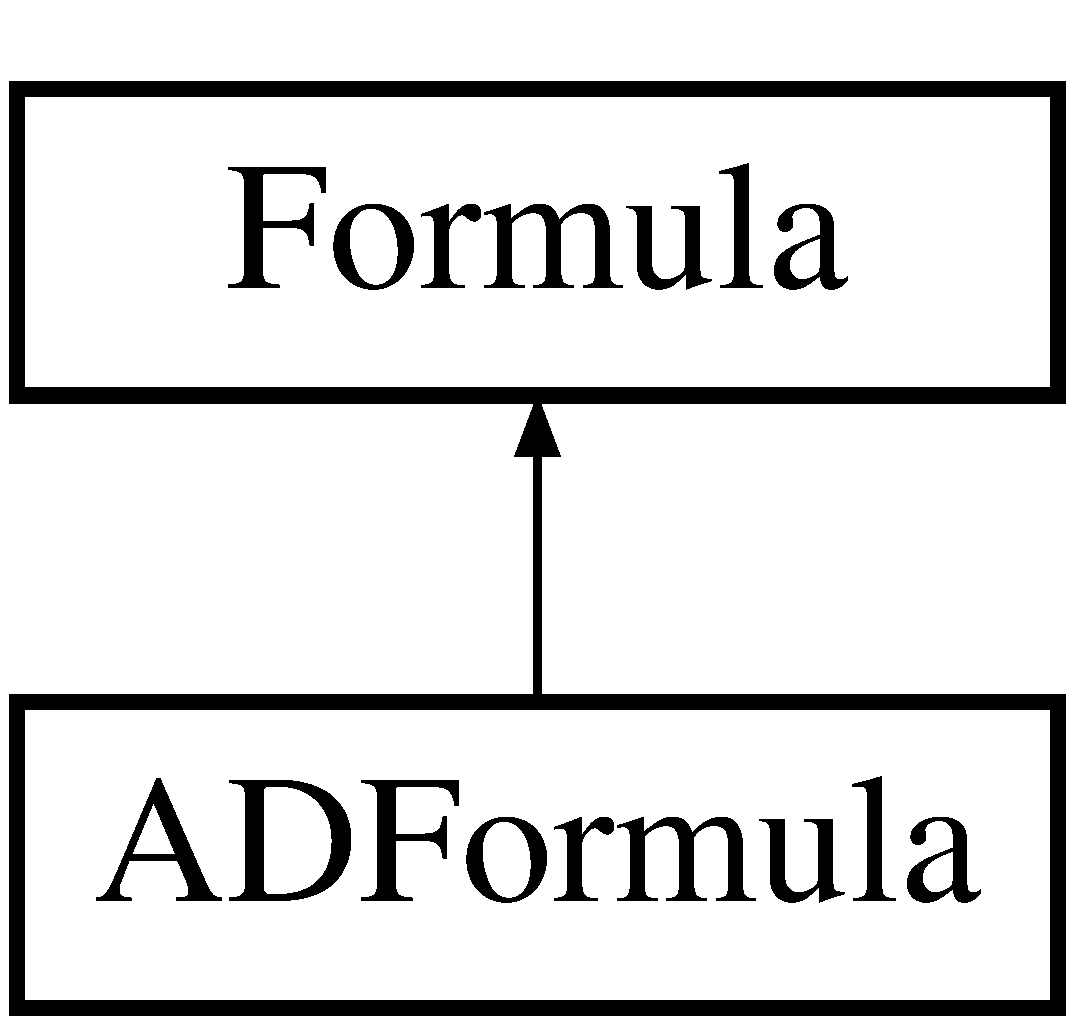
\includegraphics[height=2.000000cm]{classADFormula}
\end{center}
\end{figure}
\subsection*{Public Member Functions}
\begin{DoxyCompactItemize}
\item 
\hypertarget{classADFormula_a38f6414a37db523ad0aa8d162912af2d}{{\bfseries A\-D\-Formula} (\hyperlink{classAtomContFormula}{Atom\-Cont\-Formula} $\ast$cont, \hyperlink{classAtomDisFormula}{Atom\-Dis\-Formula} $\ast$dis)}\label{classADFormula_a38f6414a37db523ad0aa8d162912af2d}

\item 
\hypertarget{classADFormula_a9b4c832de720b908226fe618f1f3c4a5}{Formula\-\_\-type {\bfseries get\-Type} ()}\label{classADFormula_a9b4c832de720b908226fe618f1f3c4a5}

\end{DoxyCompactItemize}
\subsection*{Public Attributes}
\begin{DoxyCompactItemize}
\item 
\hypertarget{classADFormula_a1ecce42177dbf52c447e2e8aa1316848}{\hyperlink{classAtomContFormula}{Atom\-Cont\-Formula} $\ast$ {\bfseries cont\-Formula}}\label{classADFormula_a1ecce42177dbf52c447e2e8aa1316848}

\item 
\hypertarget{classADFormula_a5d468953085cf2fb857eca9851c3e107}{\hyperlink{classAtomDisFormula}{Atom\-Dis\-Formula} $\ast$ {\bfseries dis\-Formula}}\label{classADFormula_a5d468953085cf2fb857eca9851c3e107}

\end{DoxyCompactItemize}


The documentation for this class was generated from the following file\-:\begin{DoxyCompactItemize}
\item 
model/Formula.\-h\end{DoxyCompactItemize}

\hypertarget{structArc}{\section{Arc Struct Reference}
\label{structArc}\index{Arc@{Arc}}
}
\subsection*{Public Attributes}
\begin{DoxyCompactItemize}
\item 
\hypertarget{structArc_a38b5c5e6f59aee0edbb3e4e9dcdf8c9d}{int {\bfseries type}}\label{structArc_a38b5c5e6f59aee0edbb3e4e9dcdf8c9d}

\item 
\hypertarget{structArc_adf50e7b02ba35f13b43aba9d5e47777c}{char $\ast$ {\bfseries id}}\label{structArc_adf50e7b02ba35f13b43aba9d5e47777c}

\item 
\hypertarget{structArc_adc4d66f6bb535697e96d138027f92651}{int {\bfseries from\-Id}}\label{structArc_adc4d66f6bb535697e96d138027f92651}

\item 
\hypertarget{structArc_ae421277390b2c7353712922cbe06663d}{int {\bfseries to\-Id}}\label{structArc_ae421277390b2c7353712922cbe06663d}

\item 
\hypertarget{structArc_aa19dfdb1931d6c21730c079711592cf9}{double {\bfseries weight}}\label{structArc_aa19dfdb1931d6c21730c079711592cf9}

\item 
\hypertarget{structArc_aba00cfe2149fe72b3925cd4398a9bc2d}{double {\bfseries share}}\label{structArc_aba00cfe2149fe72b3925cd4398a9bc2d}

\item 
\hypertarget{structArc_a113c9b55b1459477681c4e8f36c2df56}{int {\bfseries priority}}\label{structArc_a113c9b55b1459477681c4e8f36c2df56}

\item 
\hypertarget{structArc_a296eec4d4ed5adb0e239679807e56f8e}{int {\bfseries trans\-Id}}\label{structArc_a296eec4d4ed5adb0e239679807e56f8e}

\item 
\hypertarget{structArc_a045db84eb3c5fffecbd0354f55d03097}{int {\bfseries place\-Id}}\label{structArc_a045db84eb3c5fffecbd0354f55d03097}

\end{DoxyCompactItemize}


The documentation for this struct was generated from the following files\-:\begin{DoxyCompactItemize}
\item 
model/D\-F\-P\-N2.\-h\item 
model/old/D\-F\-P\-N2.\-h\end{DoxyCompactItemize}

\hypertarget{classAtomContFormula}{\section{Atom\-Cont\-Formula Class Reference}
\label{classAtomContFormula}\index{Atom\-Cont\-Formula@{Atom\-Cont\-Formula}}
}
Inheritance diagram for Atom\-Cont\-Formula\-:\begin{figure}[H]
\begin{center}
\leavevmode
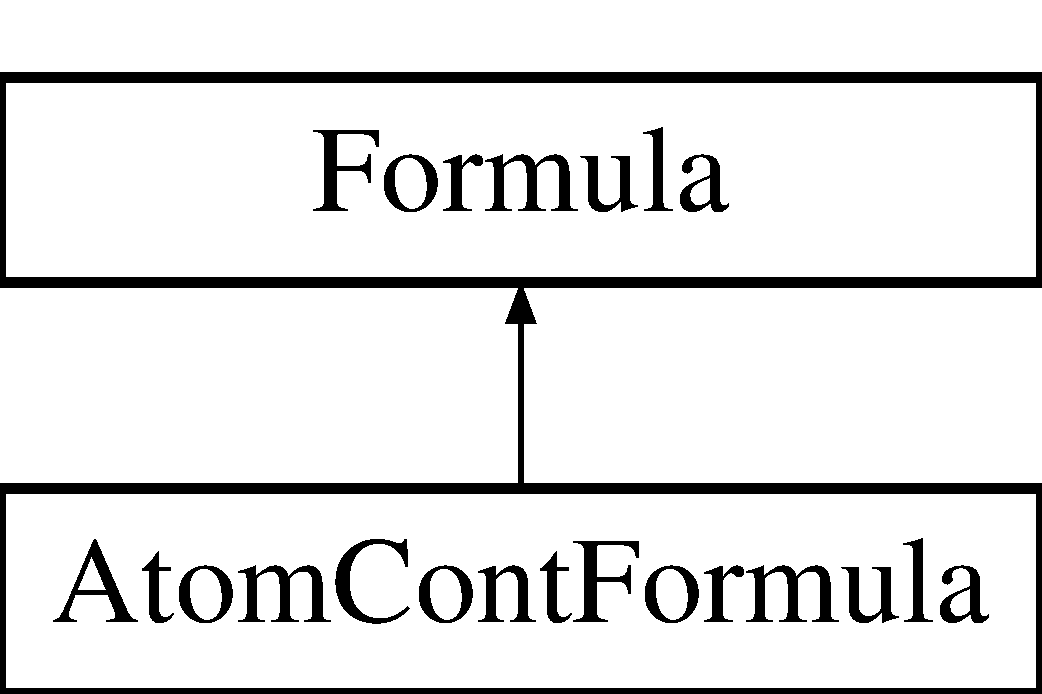
\includegraphics[height=2.000000cm]{classAtomContFormula}
\end{center}
\end{figure}
\subsection*{Public Member Functions}
\begin{DoxyCompactItemize}
\item 
\hyperlink{classAtomContFormula_a57d79f06baad31ddb734cb1b7ac128bb}{Atom\-Cont\-Formula} (unsigned int \-\_\-place\-Index, double \-\_\-c)
\begin{DoxyCompactList}\small\item\em Contains atomic formula of type $x \geq c $. \end{DoxyCompactList}\item 
\hypertarget{classAtomContFormula_a31fc3eea53c83452f05294e6d72ef819}{Formula\-\_\-type {\bfseries get\-Type} ()}\label{classAtomContFormula_a31fc3eea53c83452f05294e6d72ef819}

\item 
\hypertarget{classAtomContFormula_af119aa721b68f164fadca6e45361c221}{double {\bfseries get\-C} () const }\label{classAtomContFormula_af119aa721b68f164fadca6e45361c221}

\item 
\hypertarget{classAtomContFormula_afdc6917482500a40d8cdbef6a6ab1d8b}{unsigned int {\bfseries get\-Place\-Index} () const }\label{classAtomContFormula_afdc6917482500a40d8cdbef6a6ab1d8b}

\end{DoxyCompactItemize}


\subsection{Constructor \& Destructor Documentation}
\hypertarget{classAtomContFormula_a57d79f06baad31ddb734cb1b7ac128bb}{\index{Atom\-Cont\-Formula@{Atom\-Cont\-Formula}!Atom\-Cont\-Formula@{Atom\-Cont\-Formula}}
\index{Atom\-Cont\-Formula@{Atom\-Cont\-Formula}!AtomContFormula@{Atom\-Cont\-Formula}}
\subsubsection[{Atom\-Cont\-Formula}]{\setlength{\rightskip}{0pt plus 5cm}Atom\-Cont\-Formula\-::\-Atom\-Cont\-Formula (
\begin{DoxyParamCaption}
\item[{unsigned int}]{\-\_\-place\-Index, }
\item[{double}]{\-\_\-c}
\end{DoxyParamCaption}
)\hspace{0.3cm}{\ttfamily [inline]}}}\label{classAtomContFormula_a57d79f06baad31ddb734cb1b7ac128bb}


Contains atomic formula of type $x \geq c $. 


\begin{DoxyParams}{Parameters}
{\em place\-Index} & index of place $ x $. \\
\hline
{\em c} & camparison value. \\
\hline
\end{DoxyParams}


The documentation for this class was generated from the following file\-:\begin{DoxyCompactItemize}
\item 
model/Formula.\-h\end{DoxyCompactItemize}

\hypertarget{classAtomDisFormula}{\section{Atom\-Dis\-Formula Class Reference}
\label{classAtomDisFormula}\index{Atom\-Dis\-Formula@{Atom\-Dis\-Formula}}
}
Inheritance diagram for Atom\-Dis\-Formula\-:\begin{figure}[H]
\begin{center}
\leavevmode
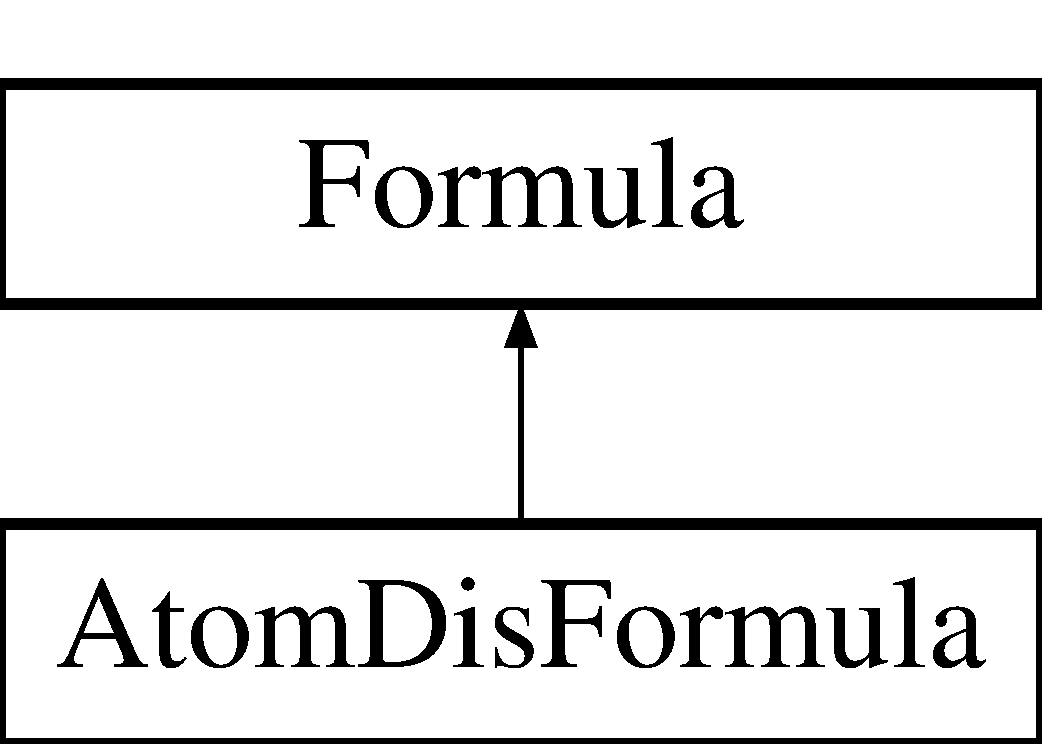
\includegraphics[height=2.000000cm]{classAtomDisFormula}
\end{center}
\end{figure}
\subsection*{Public Member Functions}
\begin{DoxyCompactItemize}
\item 
\hypertarget{classAtomDisFormula_ad9f872e92df52655d165ff9a01308331}{{\bfseries Atom\-Dis\-Formula} (unsigned int \-\_\-place\-Index, int \-\_\-n)}\label{classAtomDisFormula_ad9f872e92df52655d165ff9a01308331}

\item 
\hypertarget{classAtomDisFormula_ad0170c8eb8d835a2a5a5544b27bf5e6a}{Formula\-\_\-type {\bfseries get\-Type} ()}\label{classAtomDisFormula_ad0170c8eb8d835a2a5a5544b27bf5e6a}

\item 
\hypertarget{classAtomDisFormula_aa2e45ee43ca473e5388f4cff731b0e44}{int {\bfseries get\-N} () const }\label{classAtomDisFormula_aa2e45ee43ca473e5388f4cff731b0e44}

\item 
\hypertarget{classAtomDisFormula_af7fc615a88b6c197a59e873a62cc7d61}{unsigned int {\bfseries get\-Place\-Index} () const }\label{classAtomDisFormula_af7fc615a88b6c197a59e873a62cc7d61}

\end{DoxyCompactItemize}


The documentation for this class was generated from the following file\-:\begin{DoxyCompactItemize}
\item 
model/Formula.\-h\end{DoxyCompactItemize}

\hypertarget{classCalculator}{\section{Calculator Class Reference}
\label{classCalculator}\index{Calculator@{Calculator}}
}
\subsection*{Public Member Functions}
\begin{DoxyCompactItemize}
\item 
\hypertarget{classCalculator_a824ab5b5f701d31a1300e6dcee9ef5c4}{{\bfseries Calculator} (Q\-String raw\-File\-Name, Q\-String raw\-Place\-Name, \hyperlink{classGUIController}{G\-U\-I\-Controller} $\ast$guic)}\label{classCalculator_a824ab5b5f701d31a1300e6dcee9ef5c4}

\item 
\hypertarget{classCalculator_a6a6894287322ae2b651224ffe180d648}{virtual bool {\bfseries set\-Place} (Q\-String raw\-Place\-Name)}\label{classCalculator_a6a6894287322ae2b651224ffe180d648}

\item 
\hypertarget{classCalculator_a832e1f4bffc5758d934e391ec733ffbc}{virtual bool {\bfseries set\-File} (Q\-String raw\-File\-Name)}\label{classCalculator_a832e1f4bffc5758d934e391ec733ffbc}

\item 
\hypertarget{classCalculator_a89c07091640287ae63320233179b9e41}{virtual bool {\bfseries show\-S\-T\-D} (Q\-String raw\-File\-Name)}\label{classCalculator_a89c07091640287ae63320233179b9e41}

\end{DoxyCompactItemize}


The documentation for this class was generated from the following files\-:\begin{DoxyCompactItemize}
\item 
model/Calculator.\-h\item 
model/Calculator.\-cpp\end{DoxyCompactItemize}

\hypertarget{classClipperLib_1_1Clipper}{\section{Clipper\-Lib\-:\-:Clipper Class Reference}
\label{classClipperLib_1_1Clipper}\index{Clipper\-Lib\-::\-Clipper@{Clipper\-Lib\-::\-Clipper}}
}
Inheritance diagram for Clipper\-Lib\-:\-:Clipper\-:\begin{figure}[H]
\begin{center}
\leavevmode
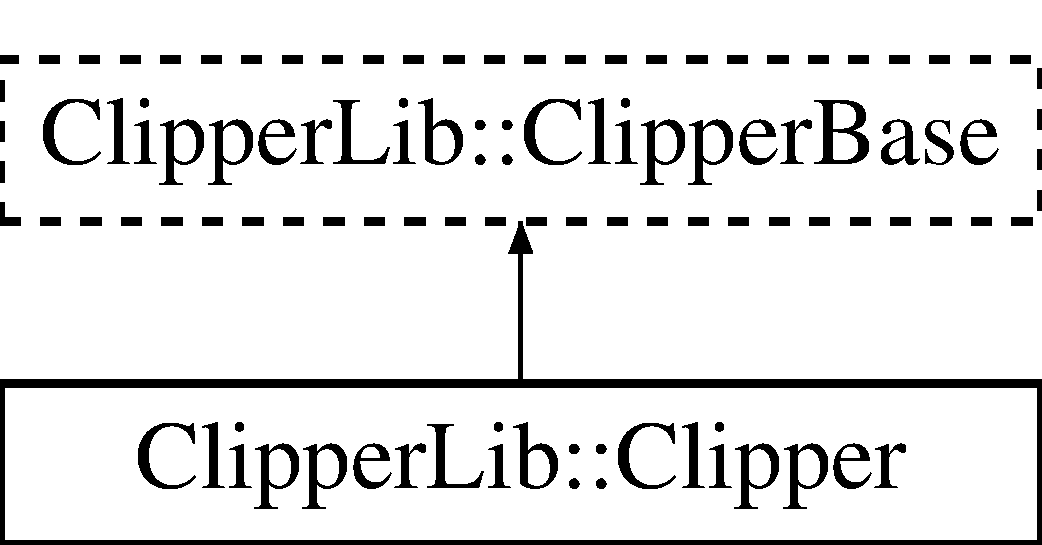
\includegraphics[height=2.000000cm]{classClipperLib_1_1Clipper}
\end{center}
\end{figure}
\subsection*{Public Member Functions}
\begin{DoxyCompactItemize}
\item 
\hypertarget{classClipperLib_1_1Clipper_a674d5d300c73a4da99bc36a7ecde0618}{bool {\bfseries Execute} (Clip\-Type clip\-Type, Polygons \&solution, Poly\-Fill\-Type subj\-Fill\-Type=pft\-Even\-Odd, Poly\-Fill\-Type clip\-Fill\-Type=pft\-Even\-Odd)}\label{classClipperLib_1_1Clipper_a674d5d300c73a4da99bc36a7ecde0618}

\item 
\hypertarget{classClipperLib_1_1Clipper_aceb19a1e5a5c9e31067f4d1177793403}{bool {\bfseries Execute} (Clip\-Type clip\-Type, \hyperlink{classClipperLib_1_1PolyTree}{Poly\-Tree} \&polytree, Poly\-Fill\-Type subj\-Fill\-Type=pft\-Even\-Odd, Poly\-Fill\-Type clip\-Fill\-Type=pft\-Even\-Odd)}\label{classClipperLib_1_1Clipper_aceb19a1e5a5c9e31067f4d1177793403}

\item 
\hypertarget{classClipperLib_1_1Clipper_a4f4576bad48bce34a36e6806623abd7a}{void {\bfseries Clear} ()}\label{classClipperLib_1_1Clipper_a4f4576bad48bce34a36e6806623abd7a}

\item 
\hypertarget{classClipperLib_1_1Clipper_ad556ba9961f498de02d55dc95bc5a889}{bool {\bfseries Reverse\-Solution} ()}\label{classClipperLib_1_1Clipper_ad556ba9961f498de02d55dc95bc5a889}

\item 
\hypertarget{classClipperLib_1_1Clipper_a44afc0c82a1d2607829b5fd21f7644ef}{void {\bfseries Reverse\-Solution} (bool value)}\label{classClipperLib_1_1Clipper_a44afc0c82a1d2607829b5fd21f7644ef}

\end{DoxyCompactItemize}
\subsection*{Protected Member Functions}
\begin{DoxyCompactItemize}
\item 
\hypertarget{classClipperLib_1_1Clipper_a14c704b062e8a079e34a8ce40838861e}{void {\bfseries Reset} ()}\label{classClipperLib_1_1Clipper_a14c704b062e8a079e34a8ce40838861e}

\item 
\hypertarget{classClipperLib_1_1Clipper_a3e8757e5f8a6ffcb7fd0f9630fde02d3}{virtual bool {\bfseries Execute\-Internal} ()}\label{classClipperLib_1_1Clipper_a3e8757e5f8a6ffcb7fd0f9630fde02d3}

\end{DoxyCompactItemize}
\subsection*{Additional Inherited Members}


The documentation for this class was generated from the following files\-:\begin{DoxyCompactItemize}
\item 
model/clipper/clipper.\-hpp\item 
model/clipper/clipper.\-cpp\end{DoxyCompactItemize}

\hypertarget{classClipperLib_1_1ClipperBase}{\section{Clipper\-Lib\-:\-:Clipper\-Base Class Reference}
\label{classClipperLib_1_1ClipperBase}\index{Clipper\-Lib\-::\-Clipper\-Base@{Clipper\-Lib\-::\-Clipper\-Base}}
}
Inheritance diagram for Clipper\-Lib\-:\-:Clipper\-Base\-:\begin{figure}[H]
\begin{center}
\leavevmode
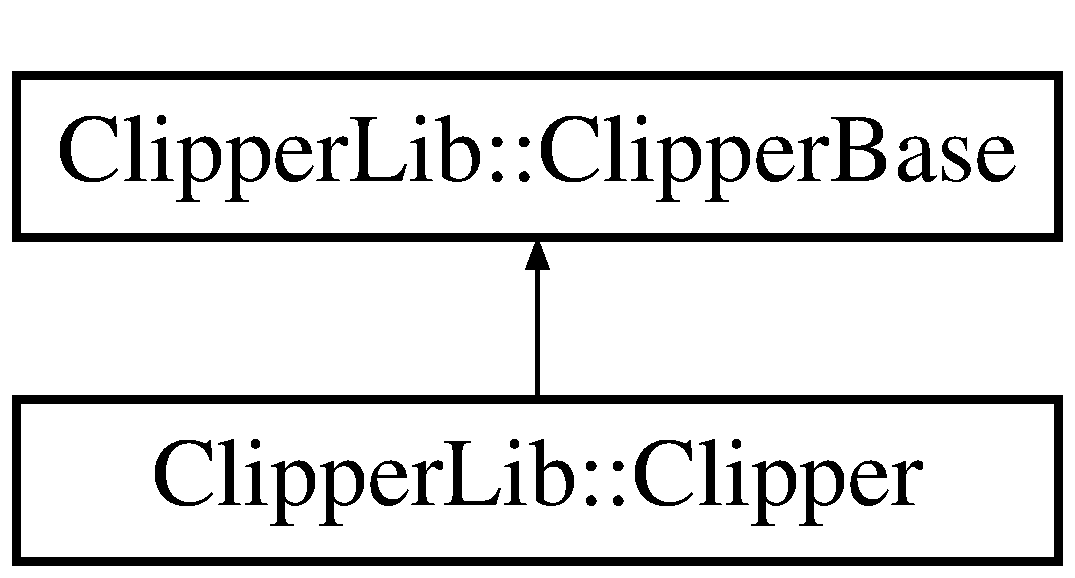
\includegraphics[height=2.000000cm]{classClipperLib_1_1ClipperBase}
\end{center}
\end{figure}
\subsection*{Public Member Functions}
\begin{DoxyCompactItemize}
\item 
\hypertarget{classClipperLib_1_1ClipperBase_a62f7b073052eed2d0ee9af69a237badd}{bool {\bfseries Add\-Polygon} (const \hyperlink{classPolygon}{Polygon} \&pg, Poly\-Type poly\-Type)}\label{classClipperLib_1_1ClipperBase_a62f7b073052eed2d0ee9af69a237badd}

\item 
\hypertarget{classClipperLib_1_1ClipperBase_a5cdf386f8ba72b196dec6ad0a8607bbf}{bool {\bfseries Add\-Polygons} (const Polygons \&ppg, Poly\-Type poly\-Type)}\label{classClipperLib_1_1ClipperBase_a5cdf386f8ba72b196dec6ad0a8607bbf}

\item 
\hypertarget{classClipperLib_1_1ClipperBase_a5690952fe8c2cb047025566405827821}{virtual void {\bfseries Clear} ()}\label{classClipperLib_1_1ClipperBase_a5690952fe8c2cb047025566405827821}

\item 
\hypertarget{classClipperLib_1_1ClipperBase_a5590a5454248ac3f6beeba7f9690f62e}{\hyperlink{structClipperLib_1_1IntRect}{Int\-Rect} {\bfseries Get\-Bounds} ()}\label{classClipperLib_1_1ClipperBase_a5590a5454248ac3f6beeba7f9690f62e}

\end{DoxyCompactItemize}
\subsection*{Protected Member Functions}
\begin{DoxyCompactItemize}
\item 
\hypertarget{classClipperLib_1_1ClipperBase_a311dbbec1454ab7965e363a0359f5ee4}{void {\bfseries Dispose\-Local\-Minima\-List} ()}\label{classClipperLib_1_1ClipperBase_a311dbbec1454ab7965e363a0359f5ee4}

\item 
\hypertarget{classClipperLib_1_1ClipperBase_a2e70686545484c6767dead34d9673ebe}{\hyperlink{structClipperLib_1_1TEdge}{T\-Edge} $\ast$ {\bfseries Add\-Bounds\-To\-L\-M\-L} (\hyperlink{structClipperLib_1_1TEdge}{T\-Edge} $\ast$e)}\label{classClipperLib_1_1ClipperBase_a2e70686545484c6767dead34d9673ebe}

\item 
\hypertarget{classClipperLib_1_1ClipperBase_a9554e9f2273c39e0f5f07d3cd73533e6}{void {\bfseries Pop\-Local\-Minima} ()}\label{classClipperLib_1_1ClipperBase_a9554e9f2273c39e0f5f07d3cd73533e6}

\item 
\hypertarget{classClipperLib_1_1ClipperBase_a125febb065f23fc55dafffe8d185b642}{virtual void {\bfseries Reset} ()}\label{classClipperLib_1_1ClipperBase_a125febb065f23fc55dafffe8d185b642}

\item 
\hypertarget{classClipperLib_1_1ClipperBase_aa62506f423172bccd6de8a645cc29cff}{void {\bfseries Insert\-Local\-Minima} (\hyperlink{structClipperLib_1_1LocalMinima}{Local\-Minima} $\ast$new\-Lm)}\label{classClipperLib_1_1ClipperBase_aa62506f423172bccd6de8a645cc29cff}

\end{DoxyCompactItemize}
\subsection*{Protected Attributes}
\begin{DoxyCompactItemize}
\item 
\hypertarget{classClipperLib_1_1ClipperBase_a4e3039382d3c8ec6f9ab434021be8d43}{\hyperlink{structClipperLib_1_1LocalMinima}{Local\-Minima} $\ast$ {\bfseries m\-\_\-\-Current\-L\-M}}\label{classClipperLib_1_1ClipperBase_a4e3039382d3c8ec6f9ab434021be8d43}

\item 
\hypertarget{classClipperLib_1_1ClipperBase_a74df45b228436fa0243b53cc00192a5f}{\hyperlink{structClipperLib_1_1LocalMinima}{Local\-Minima} $\ast$ {\bfseries m\-\_\-\-Minima\-List}}\label{classClipperLib_1_1ClipperBase_a74df45b228436fa0243b53cc00192a5f}

\item 
\hypertarget{classClipperLib_1_1ClipperBase_aea11d183617adc12d7ba2b84533f7f45}{bool {\bfseries m\-\_\-\-Use\-Full\-Range}}\label{classClipperLib_1_1ClipperBase_aea11d183617adc12d7ba2b84533f7f45}

\item 
\hypertarget{classClipperLib_1_1ClipperBase_a8bfc007c0c0afd4e9d252dac0ef5daa0}{Edge\-List {\bfseries m\-\_\-edges}}\label{classClipperLib_1_1ClipperBase_a8bfc007c0c0afd4e9d252dac0ef5daa0}

\end{DoxyCompactItemize}


The documentation for this class was generated from the following files\-:\begin{DoxyCompactItemize}
\item 
model/clipper/clipper.\-hpp\item 
model/clipper/clipper.\-cpp\end{DoxyCompactItemize}

\hypertarget{classClipperLib_1_1clipperException}{\section{Clipper\-Lib\-:\-:clipper\-Exception Class Reference}
\label{classClipperLib_1_1clipperException}\index{Clipper\-Lib\-::clipper\-Exception@{Clipper\-Lib\-::clipper\-Exception}}
}
Inheritance diagram for Clipper\-Lib\-:\-:clipper\-Exception\-:\begin{figure}[H]
\begin{center}
\leavevmode
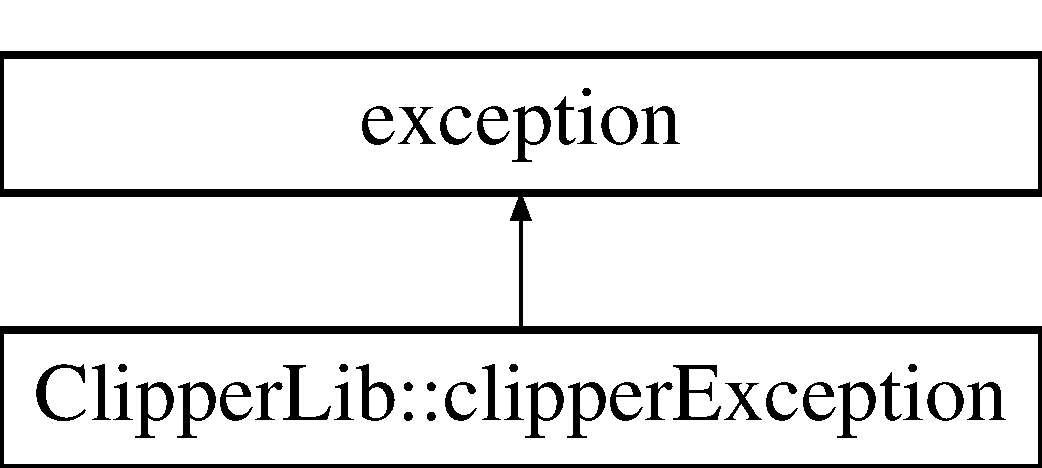
\includegraphics[height=2.000000cm]{classClipperLib_1_1clipperException}
\end{center}
\end{figure}
\subsection*{Public Member Functions}
\begin{DoxyCompactItemize}
\item 
\hypertarget{classClipperLib_1_1clipperException_a7d44b32d06cd870500355667f6e0d6ed}{{\bfseries clipper\-Exception} (const char $\ast$description)}\label{classClipperLib_1_1clipperException_a7d44b32d06cd870500355667f6e0d6ed}

\item 
\hypertarget{classClipperLib_1_1clipperException_a7bd8c881bda597f839670dde97fe04d4}{virtual const char $\ast$ {\bfseries what} () const   throw ()}\label{classClipperLib_1_1clipperException_a7bd8c881bda597f839670dde97fe04d4}

\end{DoxyCompactItemize}


The documentation for this class was generated from the following file\-:\begin{DoxyCompactItemize}
\item 
model/clipper/clipper.\-hpp\end{DoxyCompactItemize}

\hypertarget{structClipperLib_1_1DoublePoint}{\section{Clipper\-Lib\-:\-:Double\-Point Struct Reference}
\label{structClipperLib_1_1DoublePoint}\index{Clipper\-Lib\-::\-Double\-Point@{Clipper\-Lib\-::\-Double\-Point}}
}
\subsection*{Public Member Functions}
\begin{DoxyCompactItemize}
\item 
\hypertarget{structClipperLib_1_1DoublePoint_a3ccbea6aaf488e0a2d8ac499d2676093}{{\bfseries Double\-Point} (double x=0, double y=0)}\label{structClipperLib_1_1DoublePoint_a3ccbea6aaf488e0a2d8ac499d2676093}

\end{DoxyCompactItemize}
\subsection*{Public Attributes}
\begin{DoxyCompactItemize}
\item 
\hypertarget{structClipperLib_1_1DoublePoint_a675837cc05f20447313789b82d84ad31}{double {\bfseries X}}\label{structClipperLib_1_1DoublePoint_a675837cc05f20447313789b82d84ad31}

\item 
\hypertarget{structClipperLib_1_1DoublePoint_a49774a93540882d88448badf37034454}{double {\bfseries Y}}\label{structClipperLib_1_1DoublePoint_a49774a93540882d88448badf37034454}

\end{DoxyCompactItemize}


The documentation for this struct was generated from the following file\-:\begin{DoxyCompactItemize}
\item 
model/clipper/clipper.\-cpp\end{DoxyCompactItemize}

\hypertarget{structDtrmEvent}{\section{Dtrm\-Event Struct Reference}
\label{structDtrmEvent}\index{Dtrm\-Event@{Dtrm\-Event}}
}


{\ttfamily \#include $<$Event.\-h$>$}

\subsection*{Public Member Functions}
\begin{DoxyCompactItemize}
\item 
\hypertarget{structDtrmEvent_a9ff83f26140ece31d58b6f9ea33fc0ec}{{\bfseries Dtrm\-Event} (Event\-Type type)}\label{structDtrmEvent_a9ff83f26140ece31d58b6f9ea33fc0ec}

\item 
\hypertarget{structDtrmEvent_a9ff83f26140ece31d58b6f9ea33fc0ec}{{\bfseries Dtrm\-Event} (Event\-Type type)}\label{structDtrmEvent_a9ff83f26140ece31d58b6f9ea33fc0ec}

\end{DoxyCompactItemize}
\subsection*{Public Attributes}
\begin{DoxyCompactItemize}
\item 
\hypertarget{structDtrmEvent_a15d88c4e3e37f6e2f81ea826e4bce5dd}{Event\-Type {\bfseries event\-Type}}\label{structDtrmEvent_a15d88c4e3e37f6e2f81ea826e4bce5dd}

\item 
int \hyperlink{structDtrmEvent_ab5e19522a82d496b8a66791bce168d81}{id}
\item 
double \hyperlink{structDtrmEvent_a23d94e3ab2a80c673f5e42aac1b6ecb0}{time}
\item 
\hyperlink{structMarking}{Marking} $\ast$ \hyperlink{structDtrmEvent_acaa9ee345f104aee09a01fe0594eab70}{pre\-Region\-Marking}
\item 
\hypertarget{structDtrmEvent_a2fd402a2460e7cc074a3351e82eb40dd}{\hyperlink{structDtrmEvent}{Dtrm\-Event} $\ast$ {\bfseries next\-Dtrm\-Event}}\label{structDtrmEvent_a2fd402a2460e7cc074a3351e82eb40dd}

\item 
\hypertarget{structDtrmEvent_a5f3587028a3fb59d48df3a343a4b2b45}{std\-::vector$<$ \hyperlink{classSTDRegion}{S\-T\-D\-Region} $\ast$ $>$ $\ast$ {\bfseries next\-Regions}}\label{structDtrmEvent_a5f3587028a3fb59d48df3a343a4b2b45}

\item 
\hyperlink{structMarking}{Marking} $\ast$ \hyperlink{structDtrmEvent_adb35b6b002efbadbb2c01c36ff9bffb0}{post\-Region\-Marking}
\end{DoxyCompactItemize}


\subsection{Detailed Description}
Deterministic Event. 

\subsection{Member Data Documentation}
\hypertarget{structDtrmEvent_ab5e19522a82d496b8a66791bce168d81}{\index{Dtrm\-Event@{Dtrm\-Event}!id@{id}}
\index{id@{id}!DtrmEvent@{Dtrm\-Event}}
\subsubsection[{id}]{\setlength{\rightskip}{0pt plus 5cm}int Dtrm\-Event\-::id}}\label{structDtrmEvent_ab5e19522a82d496b8a66791bce168d81}
\hyperlink{structTransition}{Transition} or place I\-D; \hypertarget{structDtrmEvent_adb35b6b002efbadbb2c01c36ff9bffb0}{\index{Dtrm\-Event@{Dtrm\-Event}!post\-Region\-Marking@{post\-Region\-Marking}}
\index{post\-Region\-Marking@{post\-Region\-Marking}!DtrmEvent@{Dtrm\-Event}}
\subsubsection[{post\-Region\-Marking}]{\setlength{\rightskip}{0pt plus 5cm}{\bf Marking} $\ast$ Dtrm\-Event\-::post\-Region\-Marking}}\label{structDtrmEvent_adb35b6b002efbadbb2c01c36ff9bffb0}
marking of region before this event happening. \hypertarget{structDtrmEvent_acaa9ee345f104aee09a01fe0594eab70}{\index{Dtrm\-Event@{Dtrm\-Event}!pre\-Region\-Marking@{pre\-Region\-Marking}}
\index{pre\-Region\-Marking@{pre\-Region\-Marking}!DtrmEvent@{Dtrm\-Event}}
\subsubsection[{pre\-Region\-Marking}]{\setlength{\rightskip}{0pt plus 5cm}{\bf Marking} $\ast$ Dtrm\-Event\-::pre\-Region\-Marking}}\label{structDtrmEvent_acaa9ee345f104aee09a01fe0594eab70}
marking of region before this event happening. \hypertarget{structDtrmEvent_a23d94e3ab2a80c673f5e42aac1b6ecb0}{\index{Dtrm\-Event@{Dtrm\-Event}!time@{time}}
\index{time@{time}!DtrmEvent@{Dtrm\-Event}}
\subsubsection[{time}]{\setlength{\rightskip}{0pt plus 5cm}double Dtrm\-Event\-::time}}\label{structDtrmEvent_a23d94e3ab2a80c673f5e42aac1b6ecb0}
Occurrence time.

Occurance time. 

The documentation for this struct was generated from the following files\-:\begin{DoxyCompactItemize}
\item 
model/Event.\-h\item 
model/old/Event.\-h\end{DoxyCompactItemize}

\hypertarget{classFormula}{\section{Formula Class Reference}
\label{classFormula}\index{Formula@{Formula}}
}
Inheritance diagram for Formula\-:\begin{figure}[H]
\begin{center}
\leavevmode
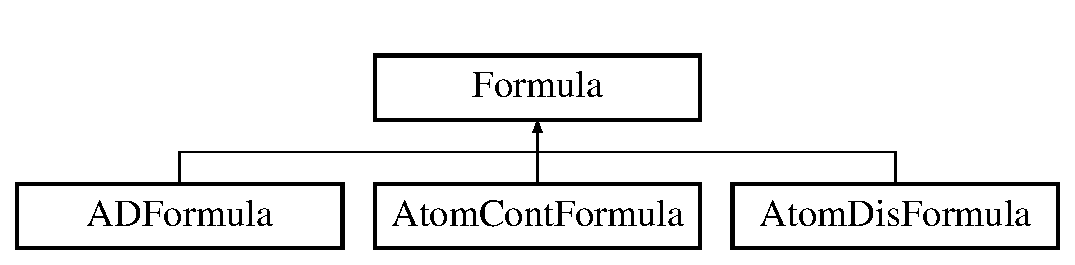
\includegraphics[height=2.000000cm]{classFormula}
\end{center}
\end{figure}
\subsection*{Public Member Functions}
\begin{DoxyCompactItemize}
\item 
\hypertarget{classFormula_aa6efa2d7eee6fc633ee30991bf11a0e0}{virtual Formula\-\_\-type {\bfseries get\-Type} ()=0}\label{classFormula_aa6efa2d7eee6fc633ee30991bf11a0e0}

\end{DoxyCompactItemize}


The documentation for this class was generated from the following file\-:\begin{DoxyCompactItemize}
\item 
model/Formula.\-h\end{DoxyCompactItemize}

\hypertarget{classGeometryHelper}{\section{Geometry\-Helper Class Reference}
\label{classGeometryHelper}\index{Geometry\-Helper@{Geometry\-Helper}}
}
\subsection*{Public Member Functions}
\begin{DoxyCompactItemize}
\item 
\hypertarget{classGeometryHelper_a23b405d720cf3806b073a406d9ae105f}{\hyperlink{classPolygon}{Polygon} $\ast$ {\bfseries create\-Polygon} (\hyperlink{classSTDRegion}{S\-T\-D\-Region} $\ast$region, \hyperlink{classFormula}{Formula} $\ast$formula)}\label{classGeometryHelper_a23b405d720cf3806b073a406d9ae105f}

\item 
\hypertarget{classGeometryHelper_a916aee5efb1bead5b9b31ae96113a740}{\hyperlink{classPolygon}{Polygon} $\ast$ {\bfseries split\-Region} (\hyperlink{classSTDRegion}{S\-T\-D\-Region} $\ast$region, \hyperlink{classLine}{Line} $\ast$line, Direction direction)}\label{classGeometryHelper_a916aee5efb1bead5b9b31ae96113a740}

\item 
\hypertarget{classGeometryHelper_aa838f64e3e5ba0bd51e974f504b46ee2}{\hyperlink{classPolygon}{Polygon} $\ast$ {\bfseries region\-To\-Poly} (\hyperlink{classSTDRegion}{S\-T\-D\-Region} $\ast$region)}\label{classGeometryHelper_aa838f64e3e5ba0bd51e974f504b46ee2}

\item 
\hypertarget{classGeometryHelper_a0c3abc152f2440a387def0530ca08b5e}{void {\bfseries add\-To\-Polygon} (\hyperlink{classPolygon}{Polygon} $\ast$poly, \hyperlink{classSegment}{Segment} $\ast$seg, \hyperlink{classLine}{Line} $\ast$line, Direction direction)}\label{classGeometryHelper_a0c3abc152f2440a387def0530ca08b5e}

\item 
\hypertarget{classGeometryHelper_ac1d7fd8e11f5613246c997efe4ad8b58}{bool {\bfseries is\-Poly\-Contain\-Pt} (\hyperlink{classPolygon}{Polygon} $\ast$poly, \hyperlink{structPoint}{Point} $\ast$p)}\label{classGeometryHelper_ac1d7fd8e11f5613246c997efe4ad8b58}

\item 
\hypertarget{classGeometryHelper_af6c198ccd6296b4f1a6bb8a019999eaf}{\hyperlink{classIntervalSet}{Interval\-Set} $\ast$ {\bfseries get\-Intersection\-Intervals} (\hyperlink{classPolygon}{Polygon} $\ast$poly, \hyperlink{classSegment}{Segment} $\ast$segment)}\label{classGeometryHelper_af6c198ccd6296b4f1a6bb8a019999eaf}

\item 
\hypertarget{classGeometryHelper_a6098e903f0a208eb07d0c5d757a4f287}{\hyperlink{classIntervalSet}{Interval\-Set} $\ast$ {\bfseries get\-Intersection\-Intervals} (\hyperlink{classPolygon}{Polygon} $\ast$poly1, \hyperlink{classPolygon}{Polygon} $\ast$poly2)}\label{classGeometryHelper_a6098e903f0a208eb07d0c5d757a4f287}

\item 
\hypertarget{classGeometryHelper_ab841a9e5157551f92b258b35256fa47c}{\hyperlink{classPolygon}{Polygon} $\ast$ {\bfseries reform} (\hyperlink{classPolygon}{Polygon} $\ast$poly, \hyperlink{classInterval}{Interval} interval)}\label{classGeometryHelper_ab841a9e5157551f92b258b35256fa47c}

\item 
\hypertarget{classGeometryHelper_aef019beba9a3b2b53003547a827cf4a3}{Region\-State {\bfseries get\-Time\-And\-Direction} (\hyperlink{structDtrmEvent}{Dtrm\-Event} $\ast$dtrm\-Region, \hyperlink{classFormula}{Formula} $\ast$psi1, double \&t, Direction \&dir)}\label{classGeometryHelper_aef019beba9a3b2b53003547a827cf4a3}

\item 
\hypertarget{classGeometryHelper_aeeb237d9828716f45df0d448a8d7d38d}{\hyperlink{classPolygon}{Polygon} $\ast$ {\bfseries crop\-Polygon} (\hyperlink{classPolygon}{Polygon} $\ast$poly, double t, Direction dir)}\label{classGeometryHelper_aeeb237d9828716f45df0d448a8d7d38d}

\item 
\hypertarget{classGeometryHelper_a46ee0f2694f41ebbb0ceffc9b5400f85}{void {\bfseries draw\-Polygon} (cv\-::\-Mat \&im, \hyperlink{classPolygon}{Polygon} $\ast$poly, const int scale, cv\-::\-Scalar color=cv\-::\-Scalar(0, 0, 255))}\label{classGeometryHelper_a46ee0f2694f41ebbb0ceffc9b5400f85}

\item 
\hypertarget{classGeometryHelper_a6af9172d08359b747bb94d345a2147de}{void {\bfseries draw\-Vertical\-Line} (cv\-::\-Mat \&im, double t, Direction dir, const int scale, cv\-::\-Scalar color=cv\-::\-Scalar(0, 0, 255))}\label{classGeometryHelper_a6af9172d08359b747bb94d345a2147de}

\item 
\hypertarget{classGeometryHelper_aeaa993b44490ab75eea883230f246a47}{{\bfseries Geometry\-Helper} (\hyperlink{structModel}{Model} $\ast$\-\_\-model)}\label{classGeometryHelper_aeaa993b44490ab75eea883230f246a47}

\end{DoxyCompactItemize}


The documentation for this class was generated from the following files\-:\begin{DoxyCompactItemize}
\item 
model/Geometry\-Helper.\-h\item 
model/Geometry\-Helper.\-cpp\end{DoxyCompactItemize}

\hypertarget{classGUIController}{\section{G\-U\-I\-Controller Class Reference}
\label{classGUIController}\index{G\-U\-I\-Controller@{G\-U\-I\-Controller}}
}
Inheritance diagram for G\-U\-I\-Controller\-:\begin{figure}[H]
\begin{center}
\leavevmode
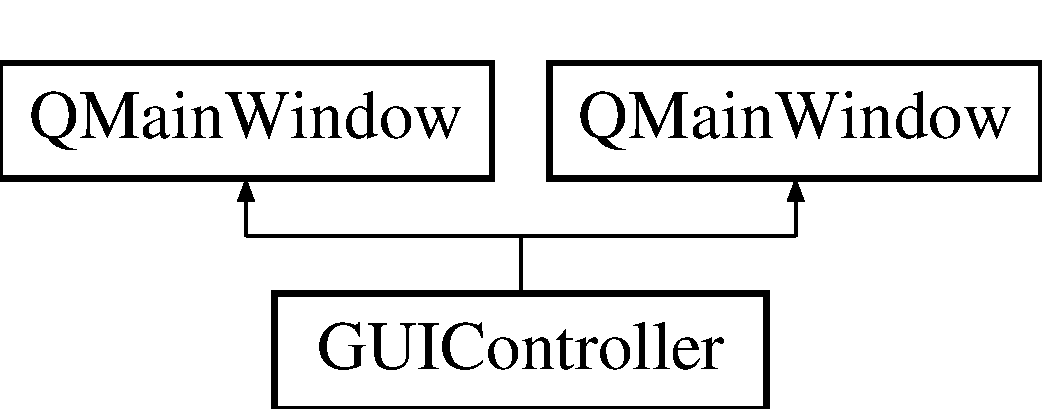
\includegraphics[height=2.000000cm]{classGUIController}
\end{center}
\end{figure}
\subsection*{Public Member Functions}
\begin{DoxyCompactItemize}
\item 
\hyperlink{classGUIController_a3f85fdeac642a3c52c0f0b586462eb8a}{G\-U\-I\-Controller} (Q\-Widget $\ast$parent=0)
\begin{DoxyCompactList}\small\item\em \hyperlink{classGUIController}{G\-U\-I\-Controller} is the constructor of the main window. The main window constructs all the elements via the ui file. The title of the main window is set to the tool name. The position of the main window is adjusted to the center. The default empty files are initiated. \end{DoxyCompactList}\item 
\hypertarget{classGUIController_acf3b4a6d7ab7be45f20ab41831644444}{\hyperlink{classGUIController_acf3b4a6d7ab7be45f20ab41831644444}{$\sim$\-G\-U\-I\-Controller} ()}\label{classGUIController_acf3b4a6d7ab7be45f20ab41831644444}

\begin{DoxyCompactList}\small\item\em The destroyer that frees the memory The ui is deleted and the memory is freed. \end{DoxyCompactList}\item 
void \hyperlink{classGUIController_a3e67be4bfe8c3ebdf943540e1b06949b}{add\-Text} (std\-::string str)
\begin{DoxyCompactList}\small\item\em Add a normal text to the build-\/in terminal. \end{DoxyCompactList}\item 
void \hyperlink{classGUIController_ac57ebab895a0f83ca9c09fd60d835585}{add\-Success} (std\-::string str)
\begin{DoxyCompactList}\small\item\em Add an success text to the build-\/in terminal. \end{DoxyCompactList}\item 
void \hyperlink{classGUIController_a5ea3697ae0408cb521e82a0b315d2661}{add\-Warning} (std\-::string str)
\begin{DoxyCompactList}\small\item\em Add a warning text to the build-\/in terminal. \end{DoxyCompactList}\item 
void \hyperlink{classGUIController_a8b5677300791307f8597dc427772ad11}{add\-Error} (std\-::string str)
\begin{DoxyCompactList}\small\item\em Add an error text to the build-\/in terminal. \end{DoxyCompactList}\item 
void \hyperlink{classGUIController_aff7752195a9d8c86d326f212ccda1e7b}{set\-Text} (std\-::string str)
\begin{DoxyCompactList}\small\item\em Set the text in the build-\/in terminal. \end{DoxyCompactList}\item 
std\-::string \hyperlink{classGUIController_a494d1c2423ce3e7d44633edc50269803}{get\-Text} ()
\begin{DoxyCompactList}\small\item\em Give the current text of the build-\/in terminal. \end{DoxyCompactList}\item 
\hypertarget{classGUIController_a3f85fdeac642a3c52c0f0b586462eb8a}{{\bfseries G\-U\-I\-Controller} (Q\-Widget $\ast$parent=0)}\label{classGUIController_a3f85fdeac642a3c52c0f0b586462eb8a}

\end{DoxyCompactItemize}
\subsection*{Protected Member Functions}
\begin{DoxyCompactItemize}
\item 
void \hyperlink{classGUIController_ae675a28ff6534f3443910cdf1c8d6603}{close\-Event} (Q\-Close\-Event $\ast$event)
\begin{DoxyCompactList}\small\item\em Check if the files are saved when the window is closed. \end{DoxyCompactList}\item 
\hypertarget{classGUIController_ae675a28ff6534f3443910cdf1c8d6603}{void {\bfseries close\-Event} (Q\-Close\-Event $\ast$event)}\label{classGUIController_ae675a28ff6534f3443910cdf1c8d6603}

\end{DoxyCompactItemize}


\subsection{Constructor \& Destructor Documentation}
\hypertarget{classGUIController_a3f85fdeac642a3c52c0f0b586462eb8a}{\index{G\-U\-I\-Controller@{G\-U\-I\-Controller}!G\-U\-I\-Controller@{G\-U\-I\-Controller}}
\index{G\-U\-I\-Controller@{G\-U\-I\-Controller}!GUIController@{G\-U\-I\-Controller}}
\subsubsection[{G\-U\-I\-Controller}]{\setlength{\rightskip}{0pt plus 5cm}G\-U\-I\-Controller\-::\-G\-U\-I\-Controller (
\begin{DoxyParamCaption}
\item[{Q\-Widget $\ast$}]{parent = {\ttfamily 0}}
\end{DoxyParamCaption}
)\hspace{0.3cm}{\ttfamily [explicit]}}}\label{classGUIController_a3f85fdeac642a3c52c0f0b586462eb8a}


\hyperlink{classGUIController}{G\-U\-I\-Controller} is the constructor of the main window. The main window constructs all the elements via the ui file. The title of the main window is set to the tool name. The position of the main window is adjusted to the center. The default empty files are initiated. 

F\-S\-T\-Gui\-::\-F\-S\-T\-Gui is the constructor of the main window. The main window constructs all the elements via the ui file. The title of the main window is set to the tool name. The position of the main window is adjusted to the center. The default empty files are initiated.


\begin{DoxyParams}{Parameters}
{\em parent} & the parent Q\-Widget \\
\hline
\end{DoxyParams}


\subsection{Member Function Documentation}
\hypertarget{classGUIController_a8b5677300791307f8597dc427772ad11}{\index{G\-U\-I\-Controller@{G\-U\-I\-Controller}!add\-Error@{add\-Error}}
\index{add\-Error@{add\-Error}!GUIController@{G\-U\-I\-Controller}}
\subsubsection[{add\-Error}]{\setlength{\rightskip}{0pt plus 5cm}void G\-U\-I\-Controller\-::add\-Error (
\begin{DoxyParamCaption}
\item[{std\-::string}]{str}
\end{DoxyParamCaption}
)\hspace{0.3cm}{\ttfamily [virtual]}}}\label{classGUIController_a8b5677300791307f8597dc427772ad11}


Add an error text to the build-\/in terminal. 

\hyperlink{classGUIController_a3e67be4bfe8c3ebdf943540e1b06949b}{G\-U\-I\-Controller\-::add\-Text} Add an error text to the build-\/in terminal.


\begin{DoxyParams}{Parameters}
{\em str} & String containing the text to be added. \\
\hline
\end{DoxyParams}


Implements \hyperlink{classmodel_1_1Logger}{model\-::\-Logger}.

\hypertarget{classGUIController_ac57ebab895a0f83ca9c09fd60d835585}{\index{G\-U\-I\-Controller@{G\-U\-I\-Controller}!add\-Success@{add\-Success}}
\index{add\-Success@{add\-Success}!GUIController@{G\-U\-I\-Controller}}
\subsubsection[{add\-Success}]{\setlength{\rightskip}{0pt plus 5cm}void G\-U\-I\-Controller\-::add\-Success (
\begin{DoxyParamCaption}
\item[{std\-::string}]{str}
\end{DoxyParamCaption}
)\hspace{0.3cm}{\ttfamily [virtual]}}}\label{classGUIController_ac57ebab895a0f83ca9c09fd60d835585}


Add an success text to the build-\/in terminal. 

\hyperlink{classGUIController_a3e67be4bfe8c3ebdf943540e1b06949b}{G\-U\-I\-Controller\-::add\-Text} Add an information text to the build-\/in terminal.


\begin{DoxyParams}{Parameters}
{\em str} & String containing the text to be added. \\
\hline
\end{DoxyParams}


Implements \hyperlink{classmodel_1_1Logger}{model\-::\-Logger}.

\hypertarget{classGUIController_a3e67be4bfe8c3ebdf943540e1b06949b}{\index{G\-U\-I\-Controller@{G\-U\-I\-Controller}!add\-Text@{add\-Text}}
\index{add\-Text@{add\-Text}!GUIController@{G\-U\-I\-Controller}}
\subsubsection[{add\-Text}]{\setlength{\rightskip}{0pt plus 5cm}void G\-U\-I\-Controller\-::add\-Text (
\begin{DoxyParamCaption}
\item[{std\-::string}]{str}
\end{DoxyParamCaption}
)\hspace{0.3cm}{\ttfamily [virtual]}}}\label{classGUIController_a3e67be4bfe8c3ebdf943540e1b06949b}


Add a normal text to the build-\/in terminal. 

\hyperlink{classGUIController_a3e67be4bfe8c3ebdf943540e1b06949b}{G\-U\-I\-Controller\-::add\-Text} Add a normal text to the build-\/in terminal.


\begin{DoxyParams}{Parameters}
{\em str} & String containing the text to be added. \\
\hline
\end{DoxyParams}


Implements \hyperlink{classmodel_1_1Logger}{model\-::\-Logger}.

\hypertarget{classGUIController_a5ea3697ae0408cb521e82a0b315d2661}{\index{G\-U\-I\-Controller@{G\-U\-I\-Controller}!add\-Warning@{add\-Warning}}
\index{add\-Warning@{add\-Warning}!GUIController@{G\-U\-I\-Controller}}
\subsubsection[{add\-Warning}]{\setlength{\rightskip}{0pt plus 5cm}void G\-U\-I\-Controller\-::add\-Warning (
\begin{DoxyParamCaption}
\item[{std\-::string}]{str}
\end{DoxyParamCaption}
)\hspace{0.3cm}{\ttfamily [virtual]}}}\label{classGUIController_a5ea3697ae0408cb521e82a0b315d2661}


Add a warning text to the build-\/in terminal. 

\hyperlink{classGUIController_a3e67be4bfe8c3ebdf943540e1b06949b}{G\-U\-I\-Controller\-::add\-Text} Add a warning text to the build-\/in terminal.


\begin{DoxyParams}{Parameters}
{\em str} & String containing the text to be added. \\
\hline
\end{DoxyParams}


Implements \hyperlink{classmodel_1_1Logger}{model\-::\-Logger}.

\hypertarget{classGUIController_ae675a28ff6534f3443910cdf1c8d6603}{\index{G\-U\-I\-Controller@{G\-U\-I\-Controller}!close\-Event@{close\-Event}}
\index{close\-Event@{close\-Event}!GUIController@{G\-U\-I\-Controller}}
\subsubsection[{close\-Event}]{\setlength{\rightskip}{0pt plus 5cm}void G\-U\-I\-Controller\-::close\-Event (
\begin{DoxyParamCaption}
\item[{Q\-Close\-Event $\ast$}]{event}
\end{DoxyParamCaption}
)\hspace{0.3cm}{\ttfamily [protected]}}}\label{classGUIController_ae675a28ff6534f3443910cdf1c8d6603}


Check if the files are saved when the window is closed. 


\begin{DoxyParams}[1]{Parameters}
\mbox{\tt out}  & {\em event} & The closing event. \\
\hline
\end{DoxyParams}
\hypertarget{classGUIController_a494d1c2423ce3e7d44633edc50269803}{\index{G\-U\-I\-Controller@{G\-U\-I\-Controller}!get\-Text@{get\-Text}}
\index{get\-Text@{get\-Text}!GUIController@{G\-U\-I\-Controller}}
\subsubsection[{get\-Text}]{\setlength{\rightskip}{0pt plus 5cm}std\-::string G\-U\-I\-Controller\-::get\-Text (
\begin{DoxyParamCaption}
{}
\end{DoxyParamCaption}
)\hspace{0.3cm}{\ttfamily [virtual]}}}\label{classGUIController_a494d1c2423ce3e7d44633edc50269803}


Give the current text of the build-\/in terminal. 

\begin{DoxyReturn}{Returns}
Gives a Q\-String text of the build-\/in terminal. 
\end{DoxyReturn}


Implements \hyperlink{classmodel_1_1Logger}{model\-::\-Logger}.

\hypertarget{classGUIController_aff7752195a9d8c86d326f212ccda1e7b}{\index{G\-U\-I\-Controller@{G\-U\-I\-Controller}!set\-Text@{set\-Text}}
\index{set\-Text@{set\-Text}!GUIController@{G\-U\-I\-Controller}}
\subsubsection[{set\-Text}]{\setlength{\rightskip}{0pt plus 5cm}void G\-U\-I\-Controller\-::set\-Text (
\begin{DoxyParamCaption}
\item[{std\-::string}]{str}
\end{DoxyParamCaption}
)\hspace{0.3cm}{\ttfamily [virtual]}}}\label{classGUIController_aff7752195a9d8c86d326f212ccda1e7b}


Set the text in the build-\/in terminal. 


\begin{DoxyParams}{Parameters}
{\em str} & String containing the text to be set. \\
\hline
\end{DoxyParams}


Implements \hyperlink{classmodel_1_1Logger}{model\-::\-Logger}.



The documentation for this class was generated from the following files\-:\begin{DoxyCompactItemize}
\item 
controller/G\-U\-I\-Controller.\-h\item 
view/G\-U\-I\-Controller.\-h\item 
controller/G\-U\-I\-Controller.\-cpp\item 
view/G\-U\-I\-Controller.\-cpp\end{DoxyCompactItemize}

\hypertarget{structClipperLib_1_1HorzJoinRec}{\section{Clipper\-Lib\-:\-:Horz\-Join\-Rec Struct Reference}
\label{structClipperLib_1_1HorzJoinRec}\index{Clipper\-Lib\-::\-Horz\-Join\-Rec@{Clipper\-Lib\-::\-Horz\-Join\-Rec}}
}
\subsection*{Public Attributes}
\begin{DoxyCompactItemize}
\item 
\hypertarget{structClipperLib_1_1HorzJoinRec_a610c6cf1e5edfc418da0965c3f68a8b8}{\hyperlink{structClipperLib_1_1TEdge}{T\-Edge} $\ast$ {\bfseries edge}}\label{structClipperLib_1_1HorzJoinRec_a610c6cf1e5edfc418da0965c3f68a8b8}

\item 
\hypertarget{structClipperLib_1_1HorzJoinRec_a58dada80e24143e14c71458340099b14}{int {\bfseries saved\-Idx}}\label{structClipperLib_1_1HorzJoinRec_a58dada80e24143e14c71458340099b14}

\end{DoxyCompactItemize}


The documentation for this struct was generated from the following file\-:\begin{DoxyCompactItemize}
\item 
model/clipper/clipper.\-hpp\end{DoxyCompactItemize}

\hypertarget{classClipperLib_1_1Int128}{\section{Clipper\-Lib\-:\-:Int128 Class Reference}
\label{classClipperLib_1_1Int128}\index{Clipper\-Lib\-::\-Int128@{Clipper\-Lib\-::\-Int128}}
}
\subsection*{Public Member Functions}
\begin{DoxyCompactItemize}
\item 
\hypertarget{classClipperLib_1_1Int128_acb7953a56e0ddb6d3245268e457f9e37}{{\bfseries Int128} (long64 \-\_\-lo=0)}\label{classClipperLib_1_1Int128_acb7953a56e0ddb6d3245268e457f9e37}

\item 
\hypertarget{classClipperLib_1_1Int128_ad113c3dc3bd371984b05fddb1fe527e2}{{\bfseries Int128} (const \hyperlink{classClipperLib_1_1Int128}{Int128} \&val)}\label{classClipperLib_1_1Int128_ad113c3dc3bd371984b05fddb1fe527e2}

\item 
\hypertarget{classClipperLib_1_1Int128_ac23a17a6a5ea143f0297b7ba0dd1830e}{{\bfseries Int128} (const long64 \&\-\_\-hi, const ulong64 \&\-\_\-lo)}\label{classClipperLib_1_1Int128_ac23a17a6a5ea143f0297b7ba0dd1830e}

\item 
\hypertarget{classClipperLib_1_1Int128_a51ef81c338951a30c55315d43bdf2690}{long64 {\bfseries operator=} (const long64 \&val)}\label{classClipperLib_1_1Int128_a51ef81c338951a30c55315d43bdf2690}

\item 
\hypertarget{classClipperLib_1_1Int128_a9a4597562962e318616a463350c68896}{bool {\bfseries operator==} (const \hyperlink{classClipperLib_1_1Int128}{Int128} \&val) const }\label{classClipperLib_1_1Int128_a9a4597562962e318616a463350c68896}

\item 
\hypertarget{classClipperLib_1_1Int128_a4b79b3e28a4012f87d03fc02969796f9}{bool {\bfseries operator!=} (const \hyperlink{classClipperLib_1_1Int128}{Int128} \&val) const }\label{classClipperLib_1_1Int128_a4b79b3e28a4012f87d03fc02969796f9}

\item 
\hypertarget{classClipperLib_1_1Int128_af34c23b86068c7f065a76dbc1d192269}{bool {\bfseries operator$>$} (const \hyperlink{classClipperLib_1_1Int128}{Int128} \&val) const }\label{classClipperLib_1_1Int128_af34c23b86068c7f065a76dbc1d192269}

\item 
\hypertarget{classClipperLib_1_1Int128_a1f875f6f5357bdb031dc4ef0d058268d}{bool {\bfseries operator$<$} (const \hyperlink{classClipperLib_1_1Int128}{Int128} \&val) const }\label{classClipperLib_1_1Int128_a1f875f6f5357bdb031dc4ef0d058268d}

\item 
\hypertarget{classClipperLib_1_1Int128_a1e8869c867b94465a5e4b54de49d6c11}{bool {\bfseries operator$>$=} (const \hyperlink{classClipperLib_1_1Int128}{Int128} \&val) const }\label{classClipperLib_1_1Int128_a1e8869c867b94465a5e4b54de49d6c11}

\item 
\hypertarget{classClipperLib_1_1Int128_a2c45d01fdcbf15015aff79d491c97416}{bool {\bfseries operator$<$=} (const \hyperlink{classClipperLib_1_1Int128}{Int128} \&val) const }\label{classClipperLib_1_1Int128_a2c45d01fdcbf15015aff79d491c97416}

\item 
\hypertarget{classClipperLib_1_1Int128_ad48a700134ab5c4e08bd53966b731950}{\hyperlink{classClipperLib_1_1Int128}{Int128} \& {\bfseries operator+=} (const \hyperlink{classClipperLib_1_1Int128}{Int128} \&rhs)}\label{classClipperLib_1_1Int128_ad48a700134ab5c4e08bd53966b731950}

\item 
\hypertarget{classClipperLib_1_1Int128_acb2d49860fb6ddf5b598ac6e15ac9521}{\hyperlink{classClipperLib_1_1Int128}{Int128} {\bfseries operator+} (const \hyperlink{classClipperLib_1_1Int128}{Int128} \&rhs) const }\label{classClipperLib_1_1Int128_acb2d49860fb6ddf5b598ac6e15ac9521}

\item 
\hypertarget{classClipperLib_1_1Int128_a7b35c74c15392ae8d48c031f750c1b28}{\hyperlink{classClipperLib_1_1Int128}{Int128} \& {\bfseries operator-\/=} (const \hyperlink{classClipperLib_1_1Int128}{Int128} \&rhs)}\label{classClipperLib_1_1Int128_a7b35c74c15392ae8d48c031f750c1b28}

\item 
\hypertarget{classClipperLib_1_1Int128_a9ab61c357c61a3f3ad5fc628e36879e2}{\hyperlink{classClipperLib_1_1Int128}{Int128} {\bfseries operator-\/} (const \hyperlink{classClipperLib_1_1Int128}{Int128} \&rhs) const }\label{classClipperLib_1_1Int128_a9ab61c357c61a3f3ad5fc628e36879e2}

\item 
\hypertarget{classClipperLib_1_1Int128_af1c84872b2d290230a0f68fb97013d4d}{\hyperlink{classClipperLib_1_1Int128}{Int128} {\bfseries operator-\/} () const }\label{classClipperLib_1_1Int128_af1c84872b2d290230a0f68fb97013d4d}

\item 
\hypertarget{classClipperLib_1_1Int128_a91718f7da0f2442e03e69b019f21dd7d}{\hyperlink{classClipperLib_1_1Int128}{Int128} {\bfseries operator/} (const \hyperlink{classClipperLib_1_1Int128}{Int128} \&rhs) const }\label{classClipperLib_1_1Int128_a91718f7da0f2442e03e69b019f21dd7d}

\item 
\hypertarget{classClipperLib_1_1Int128_a6629ebee1d059ea486c789eaa24fb994}{double {\bfseries As\-Double} () const }\label{classClipperLib_1_1Int128_a6629ebee1d059ea486c789eaa24fb994}

\end{DoxyCompactItemize}
\subsection*{Public Attributes}
\begin{DoxyCompactItemize}
\item 
\hypertarget{classClipperLib_1_1Int128_a991b9da6e53c777a94fca640e505b258}{ulong64 {\bfseries lo}}\label{classClipperLib_1_1Int128_a991b9da6e53c777a94fca640e505b258}

\item 
\hypertarget{classClipperLib_1_1Int128_a167643d0860a14fb563e055511e15e14}{long64 {\bfseries hi}}\label{classClipperLib_1_1Int128_a167643d0860a14fb563e055511e15e14}

\end{DoxyCompactItemize}


The documentation for this class was generated from the following file\-:\begin{DoxyCompactItemize}
\item 
model/clipper/clipper.\-cpp\end{DoxyCompactItemize}

\hypertarget{structClipperLib_1_1IntersectNode}{\section{Clipper\-Lib\-:\-:Intersect\-Node Struct Reference}
\label{structClipperLib_1_1IntersectNode}\index{Clipper\-Lib\-::\-Intersect\-Node@{Clipper\-Lib\-::\-Intersect\-Node}}
}
\subsection*{Public Attributes}
\begin{DoxyCompactItemize}
\item 
\hypertarget{structClipperLib_1_1IntersectNode_a9ca23b5341d4609ecb24ad7ac5eb6da4}{\hyperlink{structClipperLib_1_1TEdge}{T\-Edge} $\ast$ {\bfseries edge1}}\label{structClipperLib_1_1IntersectNode_a9ca23b5341d4609ecb24ad7ac5eb6da4}

\item 
\hypertarget{structClipperLib_1_1IntersectNode_ac32451de72e8e929bbb9704b8d330317}{\hyperlink{structClipperLib_1_1TEdge}{T\-Edge} $\ast$ {\bfseries edge2}}\label{structClipperLib_1_1IntersectNode_ac32451de72e8e929bbb9704b8d330317}

\item 
\hypertarget{structClipperLib_1_1IntersectNode_af24af801ac1e74f9200908dcad88cc30}{\hyperlink{structClipperLib_1_1IntPoint}{Int\-Point} {\bfseries pt}}\label{structClipperLib_1_1IntersectNode_af24af801ac1e74f9200908dcad88cc30}

\item 
\hypertarget{structClipperLib_1_1IntersectNode_a6534367f8cc07404d5f19230166f8c78}{\hyperlink{structClipperLib_1_1IntersectNode}{Intersect\-Node} $\ast$ {\bfseries next}}\label{structClipperLib_1_1IntersectNode_a6534367f8cc07404d5f19230166f8c78}

\end{DoxyCompactItemize}


The documentation for this struct was generated from the following file\-:\begin{DoxyCompactItemize}
\item 
model/clipper/clipper.\-hpp\end{DoxyCompactItemize}

\hypertarget{classInterval}{\section{Interval Class Reference}
\label{classInterval}\index{Interval@{Interval}}
}
\subsection*{Public Member Functions}
\begin{DoxyCompactItemize}
\item 
\hypertarget{classInterval_a8d429d3ac6f7b70133baecd1467dca1f}{{\bfseries Interval} (double \-\_\-start, double \-\_\-end)}\label{classInterval_a8d429d3ac6f7b70133baecd1467dca1f}

\item 
\hypertarget{classInterval_ab26781b302eecfc9d06dfc80be34baac}{\hyperlink{classInterval}{Interval} \& {\bfseries operator=} (const \hyperlink{classInterval}{Interval} \&in)}\label{classInterval_ab26781b302eecfc9d06dfc80be34baac}

\item 
\hypertarget{classInterval_a240cc6cdc44fd2f4715725eda900db63}{bool {\bfseries intersect} (const \hyperlink{classInterval}{Interval} \&in, \hyperlink{classInterval}{Interval} \&result)}\label{classInterval_a240cc6cdc44fd2f4715725eda900db63}

\item 
\hypertarget{classInterval_a4b68948ef478868d12f17ff4bbbd92f9}{\hyperlink{classIntervalSet}{Interval\-Set} $\ast$ {\bfseries minus} (const \hyperlink{classInterval}{Interval} \&in)}\label{classInterval_a4b68948ef478868d12f17ff4bbbd92f9}

\end{DoxyCompactItemize}
\subsection*{Public Attributes}
\begin{DoxyCompactItemize}
\item 
\hypertarget{classInterval_ae63ae31c07265309f48a39ce2472b692}{double {\bfseries start}}\label{classInterval_ae63ae31c07265309f48a39ce2472b692}

\item 
\hypertarget{classInterval_a3e157b77bf832e92c26fbe3283717d74}{double {\bfseries end}}\label{classInterval_a3e157b77bf832e92c26fbe3283717d74}

\end{DoxyCompactItemize}


The documentation for this class was generated from the following files\-:\begin{DoxyCompactItemize}
\item 
model/Interval\-Set.\-h\item 
model/Interval\-Set.\-cpp\end{DoxyCompactItemize}

\hypertarget{classIntervalSet}{\section{Interval\-Set Class Reference}
\label{classIntervalSet}\index{Interval\-Set@{Interval\-Set}}
}
\subsection*{Public Member Functions}
\begin{DoxyCompactItemize}
\item 
\hypertarget{classIntervalSet_a7f61649f6b0fdbef85e53883d35c312c}{\hyperlink{classIntervalSet}{Interval\-Set} $\ast$ {\bfseries intersect} (const \hyperlink{classIntervalSet}{Interval\-Set} $\ast$int\-Set)}\label{classIntervalSet_a7f61649f6b0fdbef85e53883d35c312c}

\item 
\hypertarget{classIntervalSet_afea4e5deb06c11f6e30fe367616a3def}{\hyperlink{classIntervalSet}{Interval\-Set} $\ast$ {\bfseries union\-With} (const \hyperlink{classIntervalSet}{Interval\-Set} $\ast$int\-Set)}\label{classIntervalSet_afea4e5deb06c11f6e30fe367616a3def}

\item 
\hypertarget{classIntervalSet_ac58c7985b4cc4f046e46195745bef87f}{\hyperlink{classIntervalSet}{Interval\-Set} $\ast$ {\bfseries minus} (const \hyperlink{classIntervalSet}{Interval\-Set} $\ast$int\-Set)}\label{classIntervalSet_ac58c7985b4cc4f046e46195745bef87f}

\item 
\hypertarget{classIntervalSet_ae485c7de02370ac6e9d13fb8ab940551}{\hyperlink{classIntervalSet}{Interval\-Set} $\ast$ {\bfseries intersect} (const \hyperlink{classInterval}{Interval} int\-Set)}\label{classIntervalSet_ae485c7de02370ac6e9d13fb8ab940551}

\item 
\hypertarget{classIntervalSet_affeaed45fc91426f5e43ac9400efa098}{\hyperlink{classIntervalSet}{Interval\-Set} $\ast$ {\bfseries union\-With} (const \hyperlink{classInterval}{Interval} int\-Set)}\label{classIntervalSet_affeaed45fc91426f5e43ac9400efa098}

\item 
\hypertarget{classIntervalSet_a33617c4739861b6a2d3fd8bbc7424b7d}{\hyperlink{classIntervalSet}{Interval\-Set} $\ast$ {\bfseries minus} (const \hyperlink{classInterval}{Interval} int\-Set)}\label{classIntervalSet_a33617c4739861b6a2d3fd8bbc7424b7d}

\item 
\hypertarget{classIntervalSet_a20270c64f71dc09269616f2c786b2099}{void {\bfseries sort} ()}\label{classIntervalSet_a20270c64f71dc09269616f2c786b2099}

\item 
\hypertarget{classIntervalSet_a14472d035db8d0feb2d1991e1e2f224d}{void {\bfseries remove\-Redundency} ()}\label{classIntervalSet_a14472d035db8d0feb2d1991e1e2f224d}

\item 
\hypertarget{classIntervalSet_a09d89c38e3bde61406db9b8165f8ce58}{void {\bfseries clear} ()}\label{classIntervalSet_a09d89c38e3bde61406db9b8165f8ce58}

\item 
\hypertarget{classIntervalSet_a4838899be6c59eb67b2312252bda712a}{bool {\bfseries is\-Empty} ()}\label{classIntervalSet_a4838899be6c59eb67b2312252bda712a}

\item 
\hypertarget{classIntervalSet_a9af0e410e6c0cd2429b52a0fb03074b6}{void {\bfseries print} (std\-::ostream \&out)}\label{classIntervalSet_a9af0e410e6c0cd2429b52a0fb03074b6}

\end{DoxyCompactItemize}
\subsection*{Public Attributes}
\begin{DoxyCompactItemize}
\item 
\hypertarget{classIntervalSet_ae2d5f918006c88865525549db6db3880}{std\-::vector$<$ \hyperlink{classInterval}{Interval} $>$ {\bfseries intervals}}\label{classIntervalSet_ae2d5f918006c88865525549db6db3880}

\end{DoxyCompactItemize}


The documentation for this class was generated from the following files\-:\begin{DoxyCompactItemize}
\item 
model/Interval\-Set.\-h\item 
model/Interval\-Set.\-cpp\end{DoxyCompactItemize}

\hypertarget{structClipperLib_1_1IntPoint}{\section{Clipper\-Lib\-:\-:Int\-Point Struct Reference}
\label{structClipperLib_1_1IntPoint}\index{Clipper\-Lib\-::\-Int\-Point@{Clipper\-Lib\-::\-Int\-Point}}
}
\subsection*{Public Member Functions}
\begin{DoxyCompactItemize}
\item 
\hypertarget{structClipperLib_1_1IntPoint_a455b8d5c7f6d4c8e5adebcac8fa11e71}{{\bfseries Int\-Point} (long64 x=0, long64 y=0)}\label{structClipperLib_1_1IntPoint_a455b8d5c7f6d4c8e5adebcac8fa11e71}

\end{DoxyCompactItemize}
\subsection*{Public Attributes}
\begin{DoxyCompactItemize}
\item 
\hypertarget{structClipperLib_1_1IntPoint_af47546895f6b0403abf4701cb00bd6fa}{long64 {\bfseries X}}\label{structClipperLib_1_1IntPoint_af47546895f6b0403abf4701cb00bd6fa}

\item 
\hypertarget{structClipperLib_1_1IntPoint_a24a7d31ef4e1a5d8a70e7e29f5429011}{long64 {\bfseries Y}}\label{structClipperLib_1_1IntPoint_a24a7d31ef4e1a5d8a70e7e29f5429011}

\end{DoxyCompactItemize}
\subsection*{Friends}
\begin{DoxyCompactItemize}
\item 
\hypertarget{structClipperLib_1_1IntPoint_a9d7a086edc8217df9f23c9c1635e2fd9}{std\-::ostream \& {\bfseries operator$<$$<$} (std\-::ostream \&s, \hyperlink{structClipperLib_1_1IntPoint}{Int\-Point} \&p)}\label{structClipperLib_1_1IntPoint_a9d7a086edc8217df9f23c9c1635e2fd9}

\end{DoxyCompactItemize}


The documentation for this struct was generated from the following file\-:\begin{DoxyCompactItemize}
\item 
model/clipper/clipper.\-hpp\end{DoxyCompactItemize}

\hypertarget{structClipperLib_1_1IntRect}{\section{Clipper\-Lib\-:\-:Int\-Rect Struct Reference}
\label{structClipperLib_1_1IntRect}\index{Clipper\-Lib\-::\-Int\-Rect@{Clipper\-Lib\-::\-Int\-Rect}}
}
\subsection*{Public Attributes}
\begin{DoxyCompactItemize}
\item 
\hypertarget{structClipperLib_1_1IntRect_a11caf77c3b6bde44fbb34107fa61a7a6}{long64 {\bfseries left}}\label{structClipperLib_1_1IntRect_a11caf77c3b6bde44fbb34107fa61a7a6}

\item 
\hypertarget{structClipperLib_1_1IntRect_ac5191ac3521b70bdf6fd7efd1f6ad55a}{long64 {\bfseries top}}\label{structClipperLib_1_1IntRect_ac5191ac3521b70bdf6fd7efd1f6ad55a}

\item 
\hypertarget{structClipperLib_1_1IntRect_a1403c5dd21df5ec2131996682d47ac0c}{long64 {\bfseries right}}\label{structClipperLib_1_1IntRect_a1403c5dd21df5ec2131996682d47ac0c}

\item 
\hypertarget{structClipperLib_1_1IntRect_ae85ebc1e77afcccaabebfead7385c6b8}{long64 {\bfseries bottom}}\label{structClipperLib_1_1IntRect_ae85ebc1e77afcccaabebfead7385c6b8}

\end{DoxyCompactItemize}


The documentation for this struct was generated from the following file\-:\begin{DoxyCompactItemize}
\item 
model/clipper/clipper.\-hpp\end{DoxyCompactItemize}

\hypertarget{structClipperLib_1_1JoinRec}{\section{Clipper\-Lib\-:\-:Join\-Rec Struct Reference}
\label{structClipperLib_1_1JoinRec}\index{Clipper\-Lib\-::\-Join\-Rec@{Clipper\-Lib\-::\-Join\-Rec}}
}
\subsection*{Public Attributes}
\begin{DoxyCompactItemize}
\item 
\hypertarget{structClipperLib_1_1JoinRec_a6104df321499a54dae6886f4c9e1f081}{\hyperlink{structClipperLib_1_1IntPoint}{Int\-Point} {\bfseries pt1a}}\label{structClipperLib_1_1JoinRec_a6104df321499a54dae6886f4c9e1f081}

\item 
\hypertarget{structClipperLib_1_1JoinRec_a4f2b81b4c5b3d7a318b336ae5a79bfbe}{\hyperlink{structClipperLib_1_1IntPoint}{Int\-Point} {\bfseries pt1b}}\label{structClipperLib_1_1JoinRec_a4f2b81b4c5b3d7a318b336ae5a79bfbe}

\item 
\hypertarget{structClipperLib_1_1JoinRec_a0182940405f04806ea1e946bf89deebf}{int {\bfseries poly1\-Idx}}\label{structClipperLib_1_1JoinRec_a0182940405f04806ea1e946bf89deebf}

\item 
\hypertarget{structClipperLib_1_1JoinRec_aed147cfa6dda75afeb0545ff8a58e28a}{\hyperlink{structClipperLib_1_1IntPoint}{Int\-Point} {\bfseries pt2a}}\label{structClipperLib_1_1JoinRec_aed147cfa6dda75afeb0545ff8a58e28a}

\item 
\hypertarget{structClipperLib_1_1JoinRec_a97e2949cf90e737e96e93fde982421d0}{\hyperlink{structClipperLib_1_1IntPoint}{Int\-Point} {\bfseries pt2b}}\label{structClipperLib_1_1JoinRec_a97e2949cf90e737e96e93fde982421d0}

\item 
\hypertarget{structClipperLib_1_1JoinRec_a0ee034c5ff30c40182e8bd399df38a7f}{int {\bfseries poly2\-Idx}}\label{structClipperLib_1_1JoinRec_a0ee034c5ff30c40182e8bd399df38a7f}

\end{DoxyCompactItemize}


The documentation for this struct was generated from the following file\-:\begin{DoxyCompactItemize}
\item 
model/clipper/clipper.\-hpp\end{DoxyCompactItemize}

\hypertarget{classLine}{\section{Line Class Reference}
\label{classLine}\index{Line@{Line}}
}


{\ttfamily \#include $<$Line.\-h$>$}

Inheritance diagram for Line\-:\begin{figure}[H]
\begin{center}
\leavevmode
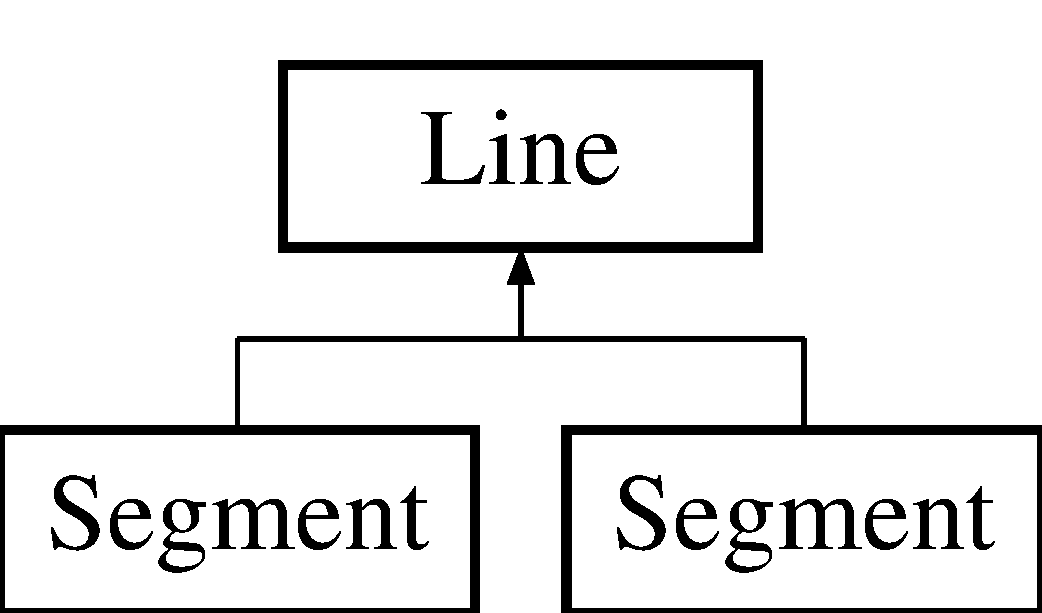
\includegraphics[height=2.000000cm]{classLine}
\end{center}
\end{figure}
\subsection*{Public Member Functions}
\begin{DoxyCompactItemize}
\item 
\hypertarget{classLine_a7a28a259e16334fce3954a07f5a7d560}{{\bfseries Line} (double \-\_\-a, double \-\_\-b)}\label{classLine_a7a28a259e16334fce3954a07f5a7d560}

\item 
\hypertarget{classLine_a82c516dfe89c6fe1f8d6c7fd4e4c3365}{{\bfseries Line} (double \-\_\-\-X)}\label{classLine_a82c516dfe89c6fe1f8d6c7fd4e4c3365}

\item 
\hypertarget{classLine_aefa59ccadcf3d41ff8eda0956fa0328e}{\hyperlink{classLine}{Line} \& {\bfseries operator=} (const \hyperlink{classLine}{Line} \&l)}\label{classLine_aefa59ccadcf3d41ff8eda0956fa0328e}

\item 
\hypertarget{classLine_a38634910f5a383f509f469e6d933460f}{\hyperlink{classLine}{Line} {\bfseries operator-\/} (const \hyperlink{classLine}{Line} \&l)}\label{classLine_a38634910f5a383f509f469e6d933460f}

\item 
double \hyperlink{classLine_a3d15d876c9e5405948078bcaa20fa1ce}{get\-Y} (double x)
\item 
\hypertarget{classLine_af7e031cb0df26db42dcd6b9dc3143378}{bool {\bfseries is\-Up} (\hyperlink{structPoint}{Point} \&p)}\label{classLine_af7e031cb0df26db42dcd6b9dc3143378}

\item 
\hypertarget{classLine_a77c4f413c7bcbb5f6b1bef061791c504}{virtual bool {\bfseries intersect} (\hyperlink{classLine}{Line} \&l, \hyperlink{structPoint}{Point} \&int\-Point)}\label{classLine_a77c4f413c7bcbb5f6b1bef061791c504}

\item 
\hypertarget{classLine_a7a28a259e16334fce3954a07f5a7d560}{{\bfseries Line} (double \-\_\-a, double \-\_\-b)}\label{classLine_a7a28a259e16334fce3954a07f5a7d560}

\item 
\hypertarget{classLine_ab29b6a1ce88c16bb1ed422ecffce61b2}{\hyperlink{classLine}{Line} \& {\bfseries operator=} (const \hyperlink{classLine}{Line} \&l)}\label{classLine_ab29b6a1ce88c16bb1ed422ecffce61b2}

\item 
\hypertarget{classLine_a38634910f5a383f509f469e6d933460f}{\hyperlink{classLine}{Line} {\bfseries operator-\/} (const \hyperlink{classLine}{Line} \&l)}\label{classLine_a38634910f5a383f509f469e6d933460f}

\item 
double \hyperlink{classLine_a3d15d876c9e5405948078bcaa20fa1ce}{get\-Y} (double x)
\item 
\hypertarget{classLine_a77c4f413c7bcbb5f6b1bef061791c504}{bool {\bfseries intersect} (\hyperlink{classLine}{Line} \&l, \hyperlink{structPoint}{Point} \&int\-Point)}\label{classLine_a77c4f413c7bcbb5f6b1bef061791c504}

\end{DoxyCompactItemize}
\subsection*{Public Attributes}
\begin{DoxyCompactItemize}
\item 
\hypertarget{classLine_aac9f3d76356545f5ab1cdc3fd52abd22}{double {\bfseries a}}\label{classLine_aac9f3d76356545f5ab1cdc3fd52abd22}

\item 
\hypertarget{classLine_ac6de6683110d1c49d6d995476fdd31ed}{double {\bfseries b}}\label{classLine_ac6de6683110d1c49d6d995476fdd31ed}

\item 
\hypertarget{classLine_a94c79256ba2c97532087fcafaa996735}{double {\bfseries X}}\label{classLine_a94c79256ba2c97532087fcafaa996735}

\end{DoxyCompactItemize}


\subsection{Detailed Description}
Represents typical line equation\-: $ y = ax + b$ (our case\-: $t = as + b$) 

\subsection{Member Function Documentation}
\hypertarget{classLine_a3d15d876c9e5405948078bcaa20fa1ce}{\index{Line@{Line}!get\-Y@{get\-Y}}
\index{get\-Y@{get\-Y}!Line@{Line}}
\subsubsection[{get\-Y}]{\setlength{\rightskip}{0pt plus 5cm}double Line\-::get\-Y (
\begin{DoxyParamCaption}
\item[{double}]{x}
\end{DoxyParamCaption}
)}}\label{classLine_a3d15d876c9e5405948078bcaa20fa1ce}
for sorting lines by their slop. \hypertarget{classLine_a3d15d876c9e5405948078bcaa20fa1ce}{\index{Line@{Line}!get\-Y@{get\-Y}}
\index{get\-Y@{get\-Y}!Line@{Line}}
\subsubsection[{get\-Y}]{\setlength{\rightskip}{0pt plus 5cm}double Line\-::get\-Y (
\begin{DoxyParamCaption}
\item[{double}]{x}
\end{DoxyParamCaption}
)}}\label{classLine_a3d15d876c9e5405948078bcaa20fa1ce}
for sorting lines by their slop. 

The documentation for this class was generated from the following files\-:\begin{DoxyCompactItemize}
\item 
model/Line.\-h\item 
model/old/Line.\-h\item 
model/Line.\-cpp\item 
model/old/Line.\-cpp\end{DoxyCompactItemize}

\hypertarget{structClipperLib_1_1LocalMinima}{\section{Clipper\-Lib\-:\-:Local\-Minima Struct Reference}
\label{structClipperLib_1_1LocalMinima}\index{Clipper\-Lib\-::\-Local\-Minima@{Clipper\-Lib\-::\-Local\-Minima}}
}
\subsection*{Public Attributes}
\begin{DoxyCompactItemize}
\item 
\hypertarget{structClipperLib_1_1LocalMinima_aa742a79c0ce808e896f28db5d5250c48}{long64 {\bfseries Y}}\label{structClipperLib_1_1LocalMinima_aa742a79c0ce808e896f28db5d5250c48}

\item 
\hypertarget{structClipperLib_1_1LocalMinima_a9325e1ed560c430a60cc677cd7c4266e}{\hyperlink{structClipperLib_1_1TEdge}{T\-Edge} $\ast$ {\bfseries left\-Bound}}\label{structClipperLib_1_1LocalMinima_a9325e1ed560c430a60cc677cd7c4266e}

\item 
\hypertarget{structClipperLib_1_1LocalMinima_a458b140addcaf1d7bc4b2fe2d3ca81f4}{\hyperlink{structClipperLib_1_1TEdge}{T\-Edge} $\ast$ {\bfseries right\-Bound}}\label{structClipperLib_1_1LocalMinima_a458b140addcaf1d7bc4b2fe2d3ca81f4}

\item 
\hypertarget{structClipperLib_1_1LocalMinima_adc944a3044f14e476f4b4ea4d5403ceb}{\hyperlink{structClipperLib_1_1LocalMinima}{Local\-Minima} $\ast$ {\bfseries next}}\label{structClipperLib_1_1LocalMinima_adc944a3044f14e476f4b4ea4d5403ceb}

\end{DoxyCompactItemize}


The documentation for this struct was generated from the following file\-:\begin{DoxyCompactItemize}
\item 
model/clipper/clipper.\-hpp\end{DoxyCompactItemize}

\hypertarget{structMarking}{\section{Marking Struct Reference}
\label{structMarking}\index{Marking@{Marking}}
}
\subsection*{Public Attributes}
\begin{DoxyCompactItemize}
\item 
\hypertarget{structMarking_adac8633ff2b18510a9b5d56228b94d5f}{int $\ast$ {\bfseries tokens}}\label{structMarking_adac8633ff2b18510a9b5d56228b94d5f}

\item 
\hypertarget{structMarking_acc070468276b4cad1f58efa182fa8a28}{double $\ast$ {\bfseries fluid0}}\label{structMarking_acc070468276b4cad1f58efa182fa8a28}

\item 
\hypertarget{structMarking_ada89f6c4febeab6d1307e57e008d3c5e}{double $\ast$ {\bfseries fluid1}}\label{structMarking_ada89f6c4febeab6d1307e57e008d3c5e}

\item 
\hypertarget{structMarking_aa967d1f3b072da5446d6da89ca7292b2}{int $\ast$ {\bfseries enabling}}\label{structMarking_aa967d1f3b072da5446d6da89ca7292b2}

\item 
\hypertarget{structMarking_a72455057a8ef90382dd01c298ccdd574}{double $\ast$ {\bfseries act\-Fluid\-Rate}}\label{structMarking_a72455057a8ef90382dd01c298ccdd574}

\item 
\hypertarget{structMarking_a407049837b4c62a64fa65182b0e6cce6}{double $\ast$ {\bfseries clock0}}\label{structMarking_a407049837b4c62a64fa65182b0e6cce6}

\item 
\hypertarget{structMarking_aff719d38a62c4809deaf4cc2b8632ed1}{double $\ast$ {\bfseries clock1}}\label{structMarking_aff719d38a62c4809deaf4cc2b8632ed1}

\item 
\hypertarget{structMarking_aa701ec8ab5d11fa7cfbc57931135fcc6}{int $\ast$ {\bfseries general\-Has\-Fired}}\label{structMarking_aa701ec8ab5d11fa7cfbc57931135fcc6}

\item 
\hypertarget{structMarking_ad5c88546dc2302b56b3b35882c738e2d}{double $\ast$ {\bfseries general\-Disabled}}\label{structMarking_ad5c88546dc2302b56b3b35882c738e2d}

\item 
\hypertarget{structMarking_a9f3e1a4d50438e41a3489ae532206f2a}{int {\bfseries N\-\_\-general\-Fired}}\label{structMarking_a9f3e1a4d50438e41a3489ae532206f2a}

\item 
\hypertarget{structMarking_ae5438ea9b802d64de9be15c12bd44bc1}{double $\ast$ {\bfseries fluid\-Place\-Deriv}}\label{structMarking_ae5438ea9b802d64de9be15c12bd44bc1}

\end{DoxyCompactItemize}


The documentation for this struct was generated from the following files\-:\begin{DoxyCompactItemize}
\item 
model/D\-F\-P\-N2.\-h\item 
model/old/D\-F\-P\-N2.\-h\end{DoxyCompactItemize}

\hypertarget{structminList}{\section{min\-List Struct Reference}
\label{structminList}\index{min\-List@{min\-List}}
}
\subsection*{Public Attributes}
\begin{DoxyCompactItemize}
\item 
\hypertarget{structminList_a8d8c249dbdaa2533613bfbd3e41d33e4}{int {\bfseries l\-Size}}\label{structminList_a8d8c249dbdaa2533613bfbd3e41d33e4}

\item 
\hypertarget{structminList_aaca30147551ec44c7ed6c3b1d2cc9567}{double $\ast$ {\bfseries split}}\label{structminList_aaca30147551ec44c7ed6c3b1d2cc9567}

\item 
\hypertarget{structminList_a3ca02a4fb0f8dfe38d879b988f5ee245}{int $\ast$ {\bfseries n\-Seg}}\label{structminList_a3ca02a4fb0f8dfe38d879b988f5ee245}

\item 
\hypertarget{structminList_a5d9e4f125a1a2dbae89c5731fd819a91}{int $\ast$$\ast$ {\bfseries min}}\label{structminList_a5d9e4f125a1a2dbae89c5731fd819a91}

\end{DoxyCompactItemize}


The documentation for this struct was generated from the following files\-:\begin{DoxyCompactItemize}
\item 
model/D\-F\-P\-N2.\-h\item 
model/old/D\-F\-P\-N2.\-h\end{DoxyCompactItemize}

\hypertarget{structModel}{\section{Model Struct Reference}
\label{structModel}\index{Model@{Model}}
}
\subsection*{Public Attributes}
\begin{DoxyCompactItemize}
\item 
\hypertarget{structModel_a660f4623c98be1f351188bb2299284d9}{int {\bfseries N\-\_\-places}}\label{structModel_a660f4623c98be1f351188bb2299284d9}

\item 
\hypertarget{structModel_a68742d9a8f4a4a93bfb3f2687ecdccb9}{\hyperlink{structPlace}{Place} $\ast$ {\bfseries places}}\label{structModel_a68742d9a8f4a4a93bfb3f2687ecdccb9}

\item 
\hypertarget{structModel_a42637d14566751b5755f2b0d66529be4}{int {\bfseries N\-\_\-transitions}}\label{structModel_a42637d14566751b5755f2b0d66529be4}

\item 
\hypertarget{structModel_abbe7678bbc58a7e1e854dcb9545ed997}{\hyperlink{structTransition}{Transition} $\ast$ {\bfseries transitions}}\label{structModel_abbe7678bbc58a7e1e854dcb9545ed997}

\item 
\hypertarget{structModel_a01029e53564beb9b1442367cf08112ee}{int {\bfseries N\-\_\-arcs}}\label{structModel_a01029e53564beb9b1442367cf08112ee}

\item 
\hypertarget{structModel_a58148ba939d857deffff97e34fb73ecd}{\hyperlink{structArc}{Arc} $\ast$ {\bfseries arcs}}\label{structModel_a58148ba939d857deffff97e34fb73ecd}

\item 
\hypertarget{structModel_a1a0417363d2111802b5615bc8ade34fa}{double {\bfseries Max\-Time}}\label{structModel_a1a0417363d2111802b5615bc8ade34fa}

\item 
\hypertarget{structModel_a6f5c61ec7dd6f557f01699824ce82927}{int {\bfseries N\-\_\-discrete\-Places}}\label{structModel_a6f5c61ec7dd6f557f01699824ce82927}

\item 
\hypertarget{structModel_af3c6151959bd7e897aa7a0cf690632fe}{int {\bfseries N\-\_\-fluid\-Places}}\label{structModel_af3c6151959bd7e897aa7a0cf690632fe}

\item 
\hypertarget{structModel_a88fb0421b5ec3b35e43d6230896b0a6f}{int {\bfseries N\-\_\-determ\-Transitions}}\label{structModel_a88fb0421b5ec3b35e43d6230896b0a6f}

\item 
\hypertarget{structModel_af930dfc6a5504ff70c34f813d95a5e82}{int {\bfseries N\-\_\-fluid\-Transitions}}\label{structModel_af930dfc6a5504ff70c34f813d95a5e82}

\item 
\hypertarget{structModel_a59d40eb8f2d1aa6afb6f46cd83d963af}{int {\bfseries N\-\_\-general\-Transitions}}\label{structModel_a59d40eb8f2d1aa6afb6f46cd83d963af}

\item 
\hypertarget{structModel_a84ea02c68790d278f5d7268fa0a7d945}{\hyperlink{structState__tag}{State} $\ast$ {\bfseries initial\-State}}\label{structModel_a84ea02c68790d278f5d7268fa0a7d945}

\end{DoxyCompactItemize}


The documentation for this struct was generated from the following files\-:\begin{DoxyCompactItemize}
\item 
model/D\-F\-P\-N2.\-h\item 
model/old/D\-F\-P\-N2.\-h\end{DoxyCompactItemize}

\hypertarget{classModelChecker}{\section{Model\-Checker Class Reference}
\label{classModelChecker}\index{Model\-Checker@{Model\-Checker}}
}
\subsection*{Public Member Functions}
\begin{DoxyCompactItemize}
\item 
\hypertarget{classModelChecker_a83460a37d9257147d4657be1d6ee8856}{{\bfseries Model\-Checker} (\hyperlink{structModel}{Model} $\ast$model, \hyperlink{classTimedDiagram}{Timed\-Diagram} $\ast$std)}\label{classModelChecker_a83460a37d9257147d4657be1d6ee8856}

\item 
\hypertarget{classModelChecker_a7cb62c308e51b561374368e357d252e8}{\hyperlink{classIntervalSet}{Interval\-Set} $\ast$ {\bfseries until} (\hyperlink{classFormula}{Formula} $\ast$psi1, \hyperlink{classFormula}{Formula} $\ast$psi2, \hyperlink{classInterval}{Interval} bound, double time)}\label{classModelChecker_a7cb62c308e51b561374368e357d252e8}

\item 
\hypertarget{classModelChecker_a23059afd44b32e1532da8a235f012dca}{double {\bfseries calc\-Prob} (\hyperlink{classIntervalSet}{Interval\-Set} $\ast$i\-Set, double($\ast$cdf)(double), double shift)}\label{classModelChecker_a23059afd44b32e1532da8a235f012dca}

\end{DoxyCompactItemize}
\subsection*{Public Attributes}
\begin{DoxyCompactItemize}
\item 
\hypertarget{classModelChecker_a5dbb1966925ec7d11656546b4a8f92e8}{cv\-::\-Mat {\bfseries debug\-Image}}\label{classModelChecker_a5dbb1966925ec7d11656546b4a8f92e8}

\item 
\hypertarget{classModelChecker_a70f70a4d5293424da22e04ae1eb59ad6}{int {\bfseries scale}}\label{classModelChecker_a70f70a4d5293424da22e04ae1eb59ad6}

\end{DoxyCompactItemize}


The documentation for this class was generated from the following files\-:\begin{DoxyCompactItemize}
\item 
model/Model\-Checker.\-h\item 
model/Model\-Checker.\-cpp\end{DoxyCompactItemize}

\hypertarget{structClipperLib_1_1OutPt}{\section{Clipper\-Lib\-:\-:Out\-Pt Struct Reference}
\label{structClipperLib_1_1OutPt}\index{Clipper\-Lib\-::\-Out\-Pt@{Clipper\-Lib\-::\-Out\-Pt}}
}
\subsection*{Public Attributes}
\begin{DoxyCompactItemize}
\item 
\hypertarget{structClipperLib_1_1OutPt_a26b2c6bbb58aeb1fb8f735f8c9724828}{int {\bfseries idx}}\label{structClipperLib_1_1OutPt_a26b2c6bbb58aeb1fb8f735f8c9724828}

\item 
\hypertarget{structClipperLib_1_1OutPt_a5caa323c71f499f356787736bdf56570}{\hyperlink{structClipperLib_1_1IntPoint}{Int\-Point} {\bfseries pt}}\label{structClipperLib_1_1OutPt_a5caa323c71f499f356787736bdf56570}

\item 
\hypertarget{structClipperLib_1_1OutPt_ac3c6f3399717ca134aaa21e6c3915cf7}{\hyperlink{structClipperLib_1_1OutPt}{Out\-Pt} $\ast$ {\bfseries next}}\label{structClipperLib_1_1OutPt_ac3c6f3399717ca134aaa21e6c3915cf7}

\item 
\hypertarget{structClipperLib_1_1OutPt_a381945867f8900451ab3c9542e9fdbab}{\hyperlink{structClipperLib_1_1OutPt}{Out\-Pt} $\ast$ {\bfseries prev}}\label{structClipperLib_1_1OutPt_a381945867f8900451ab3c9542e9fdbab}

\end{DoxyCompactItemize}


The documentation for this struct was generated from the following file\-:\begin{DoxyCompactItemize}
\item 
model/clipper/clipper.\-hpp\end{DoxyCompactItemize}

\hypertarget{structClipperLib_1_1OutRec}{\section{Clipper\-Lib\-:\-:Out\-Rec Struct Reference}
\label{structClipperLib_1_1OutRec}\index{Clipper\-Lib\-::\-Out\-Rec@{Clipper\-Lib\-::\-Out\-Rec}}
}
\subsection*{Public Attributes}
\begin{DoxyCompactItemize}
\item 
\hypertarget{structClipperLib_1_1OutRec_a86f3792d595bf0b43080973e25530325}{int {\bfseries idx}}\label{structClipperLib_1_1OutRec_a86f3792d595bf0b43080973e25530325}

\item 
\hypertarget{structClipperLib_1_1OutRec_a0d3a9a11fb66b802754f7a4709f55ed9}{bool {\bfseries is\-Hole}}\label{structClipperLib_1_1OutRec_a0d3a9a11fb66b802754f7a4709f55ed9}

\item 
\hypertarget{structClipperLib_1_1OutRec_aa8baa934f1a7687a16b88a579dec3dd4}{\hyperlink{structClipperLib_1_1OutRec}{Out\-Rec} $\ast$ {\bfseries First\-Left}}\label{structClipperLib_1_1OutRec_aa8baa934f1a7687a16b88a579dec3dd4}

\item 
\hypertarget{structClipperLib_1_1OutRec_a77fe49710e99367de8704cd570338d49}{\hyperlink{classClipperLib_1_1PolyNode}{Poly\-Node} $\ast$ {\bfseries poly\-Node}}\label{structClipperLib_1_1OutRec_a77fe49710e99367de8704cd570338d49}

\item 
\hypertarget{structClipperLib_1_1OutRec_a81021383d06dbfb7b247d053205529f2}{\hyperlink{structClipperLib_1_1OutPt}{Out\-Pt} $\ast$ {\bfseries pts}}\label{structClipperLib_1_1OutRec_a81021383d06dbfb7b247d053205529f2}

\item 
\hypertarget{structClipperLib_1_1OutRec_a81695c0c62beef7de4bbb758290ae68d}{\hyperlink{structClipperLib_1_1OutPt}{Out\-Pt} $\ast$ {\bfseries bottom\-Pt}}\label{structClipperLib_1_1OutRec_a81695c0c62beef7de4bbb758290ae68d}

\end{DoxyCompactItemize}


The documentation for this struct was generated from the following file\-:\begin{DoxyCompactItemize}
\item 
model/clipper/clipper.\-hpp\end{DoxyCompactItemize}

\hypertarget{structPlace}{\section{Place Struct Reference}
\label{structPlace}\index{Place@{Place}}
}
\subsection*{Public Attributes}
\begin{DoxyCompactItemize}
\item 
\hypertarget{structPlace_a264998153dfb8bb1f7d9202a45a1def0}{int {\bfseries type}}\label{structPlace_a264998153dfb8bb1f7d9202a45a1def0}

\item 
\hypertarget{structPlace_a441acc01591c4f77dcb5f3edff53ad03}{char $\ast$ {\bfseries id}}\label{structPlace_a441acc01591c4f77dcb5f3edff53ad03}

\item 
\hypertarget{structPlace_a638f6de89a591d32a815d80574843542}{int {\bfseries d\-\_\-mark}}\label{structPlace_a638f6de89a591d32a815d80574843542}

\item 
\hypertarget{structPlace_a528bafcfd5669c17c37967a7139d1aa2}{double {\bfseries f\-\_\-level}}\label{structPlace_a528bafcfd5669c17c37967a7139d1aa2}

\item 
\hypertarget{structPlace_abdea44022e73ec2734ca67f20bc1abb8}{double {\bfseries f\-\_\-bound}}\label{structPlace_abdea44022e73ec2734ca67f20bc1abb8}

\item 
\hypertarget{structPlace_a10b39e364e9b62f5ec688abf35c43f22}{int {\bfseries id\-In\-Marking}}\label{structPlace_a10b39e364e9b62f5ec688abf35c43f22}

\item 
\hypertarget{structPlace_a99267082e0e6e468f661688713695dd9}{int {\bfseries input\-List\-Size}}\label{structPlace_a99267082e0e6e468f661688713695dd9}

\item 
\hypertarget{structPlace_aa665e7b3206caf91f0e76c5eeeec81f2}{int $\ast$ {\bfseries input\-List}}\label{structPlace_aa665e7b3206caf91f0e76c5eeeec81f2}

\item 
\hypertarget{structPlace_ad52b3bc842fd34d1c627c77b8003c935}{int {\bfseries inhib\-List\-Size}}\label{structPlace_ad52b3bc842fd34d1c627c77b8003c935}

\item 
\hypertarget{structPlace_aa4991c973bc6fe45745746d4bffe45c3}{int $\ast$ {\bfseries inhib\-List}}\label{structPlace_aa4991c973bc6fe45745746d4bffe45c3}

\item 
\hypertarget{structPlace_a091834a116f4fa02645808754e1f907f}{int {\bfseries test\-List\-Size}}\label{structPlace_a091834a116f4fa02645808754e1f907f}

\item 
\hypertarget{structPlace_af9ab6e3e4c3deec673c65ea8fce3eac3}{int $\ast$ {\bfseries test\-List}}\label{structPlace_af9ab6e3e4c3deec673c65ea8fce3eac3}

\item 
\hypertarget{structPlace_a8a3780c3114e34e469291383511b7cd1}{int {\bfseries output\-List\-Size}}\label{structPlace_a8a3780c3114e34e469291383511b7cd1}

\item 
\hypertarget{structPlace_a6b34af9235108d743f34034e5d4af49d}{int $\ast$ {\bfseries output\-List}}\label{structPlace_a6b34af9235108d743f34034e5d4af49d}

\end{DoxyCompactItemize}


The documentation for this struct was generated from the following files\-:\begin{DoxyCompactItemize}
\item 
model/D\-F\-P\-N2.\-h\item 
model/old/D\-F\-P\-N2.\-h\end{DoxyCompactItemize}

\hypertarget{structPoint}{\section{Point Struct Reference}
\label{structPoint}\index{Point@{Point}}
}
\subsection*{Public Member Functions}
\begin{DoxyCompactItemize}
\item 
\hypertarget{structPoint_a78b55e8d5466bb8c2cf60fa55f2562ff}{{\bfseries Point} (double x, double y)}\label{structPoint_a78b55e8d5466bb8c2cf60fa55f2562ff}

\item 
\hypertarget{structPoint_a79ef74eec8fb41f7ec213beea9b1c3ac}{\hyperlink{structPoint}{Point} \& {\bfseries operator=} (const \hyperlink{structPoint}{Point} \&p)}\label{structPoint_a79ef74eec8fb41f7ec213beea9b1c3ac}

\item 
\hypertarget{structPoint_ae4c751e084aaa166a65f56788170a9e9}{bool {\bfseries operator!=} (const \hyperlink{structPoint}{Point} \&p)}\label{structPoint_ae4c751e084aaa166a65f56788170a9e9}

\item 
\hypertarget{structPoint_a1a69a0a1dea189f07e044f6eb868937d}{bool {\bfseries operator==} (const \hyperlink{structPoint}{Point} \&p)}\label{structPoint_a1a69a0a1dea189f07e044f6eb868937d}

\item 
\hypertarget{structPoint_a78b55e8d5466bb8c2cf60fa55f2562ff}{{\bfseries Point} (double x, double y)}\label{structPoint_a78b55e8d5466bb8c2cf60fa55f2562ff}

\item 
\hypertarget{structPoint_a79ef74eec8fb41f7ec213beea9b1c3ac}{\hyperlink{structPoint}{Point} \& {\bfseries operator=} (const \hyperlink{structPoint}{Point} \&p)}\label{structPoint_a79ef74eec8fb41f7ec213beea9b1c3ac}

\item 
\hypertarget{structPoint_ae4c751e084aaa166a65f56788170a9e9}{bool {\bfseries operator!=} (const \hyperlink{structPoint}{Point} \&p)}\label{structPoint_ae4c751e084aaa166a65f56788170a9e9}

\item 
\hypertarget{structPoint_a1a69a0a1dea189f07e044f6eb868937d}{bool {\bfseries operator==} (const \hyperlink{structPoint}{Point} \&p)}\label{structPoint_a1a69a0a1dea189f07e044f6eb868937d}

\end{DoxyCompactItemize}
\subsection*{Public Attributes}
\begin{DoxyCompactItemize}
\item 
\hypertarget{structPoint_a9a3d900d37caa93c8266045f9a15ddfd}{double {\bfseries X}}\label{structPoint_a9a3d900d37caa93c8266045f9a15ddfd}

\item 
\hypertarget{structPoint_afd3632a85aefc15a129a8ebc4b8412b9}{double {\bfseries Y}}\label{structPoint_afd3632a85aefc15a129a8ebc4b8412b9}

\end{DoxyCompactItemize}


The documentation for this struct was generated from the following files\-:\begin{DoxyCompactItemize}
\item 
model/Line.\-h\item 
model/old/Line.\-h\end{DoxyCompactItemize}

\hypertarget{classPolygon}{\section{Polygon Class Reference}
\label{classPolygon}\index{Polygon@{Polygon}}
}
\subsection*{Public Member Functions}
\begin{DoxyCompactItemize}
\item 
\hypertarget{classPolygon_a60830487fc3c6b815aa577e9dd758b51}{void {\bfseries print} ()}\label{classPolygon_a60830487fc3c6b815aa577e9dd758b51}

\item 
\hypertarget{classPolygon_a83cdc668a8bbc70f622cb4d18117227f}{bool {\bfseries intersect} (\hyperlink{classLine}{Line} $\ast$l, \hyperlink{structPoint}{Point} \&p1, \hyperlink{structPoint}{Point} \&p2)}\label{classPolygon_a83cdc668a8bbc70f622cb4d18117227f}

\end{DoxyCompactItemize}
\subsection*{Public Attributes}
\begin{DoxyCompactItemize}
\item 
\hypertarget{classPolygon_ae29d117eb51f45ed8f7e04f1c54bb02f}{std\-::vector$<$ \hyperlink{classSegment}{Segment} $\ast$ $>$ $\ast$ {\bfseries segments}}\label{classPolygon_ae29d117eb51f45ed8f7e04f1c54bb02f}

\end{DoxyCompactItemize}


The documentation for this class was generated from the following files\-:\begin{DoxyCompactItemize}
\item 
model/Polygon.\-h\item 
model/Polygon.\-cpp\end{DoxyCompactItemize}

\hypertarget{classClipperLib_1_1PolyNode}{\section{Clipper\-Lib\-:\-:Poly\-Node Class Reference}
\label{classClipperLib_1_1PolyNode}\index{Clipper\-Lib\-::\-Poly\-Node@{Clipper\-Lib\-::\-Poly\-Node}}
}
Inheritance diagram for Clipper\-Lib\-:\-:Poly\-Node\-:\begin{figure}[H]
\begin{center}
\leavevmode
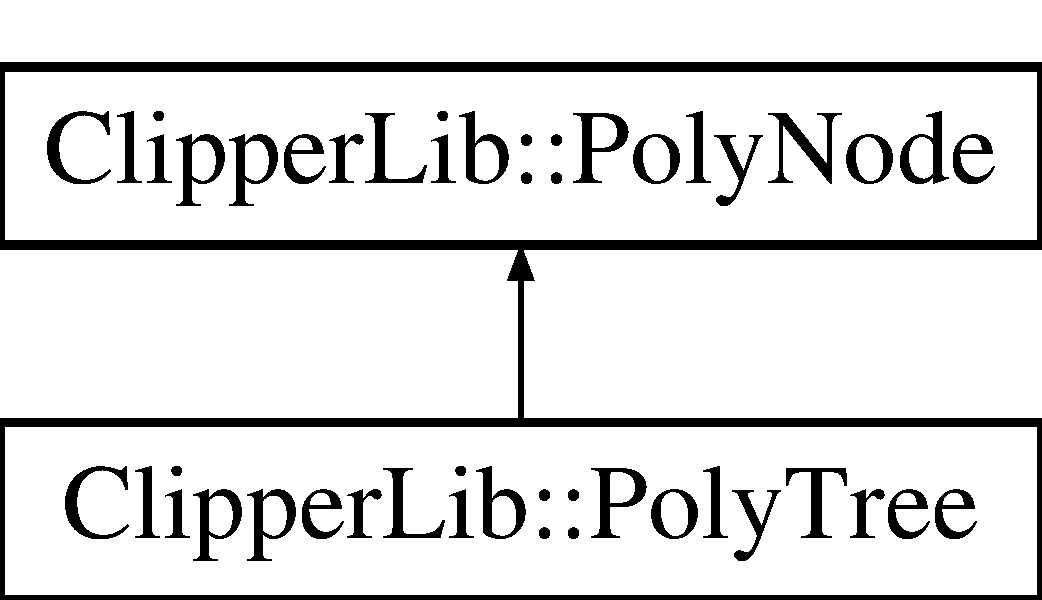
\includegraphics[height=2.000000cm]{classClipperLib_1_1PolyNode}
\end{center}
\end{figure}
\subsection*{Public Member Functions}
\begin{DoxyCompactItemize}
\item 
\hypertarget{classClipperLib_1_1PolyNode_ae9a4f50a1c9aec06c083578742d24bb7}{\hyperlink{classClipperLib_1_1PolyNode}{Poly\-Node} $\ast$ {\bfseries Get\-Next} () const }\label{classClipperLib_1_1PolyNode_ae9a4f50a1c9aec06c083578742d24bb7}

\item 
\hypertarget{classClipperLib_1_1PolyNode_aef7847f53087207b6e341c029adc1768}{bool {\bfseries Is\-Hole} () const }\label{classClipperLib_1_1PolyNode_aef7847f53087207b6e341c029adc1768}

\item 
\hypertarget{classClipperLib_1_1PolyNode_a76c8c55a45651cf3b5a67b8634173de8}{int {\bfseries Child\-Count} () const }\label{classClipperLib_1_1PolyNode_a76c8c55a45651cf3b5a67b8634173de8}

\end{DoxyCompactItemize}
\subsection*{Public Attributes}
\begin{DoxyCompactItemize}
\item 
\hypertarget{classClipperLib_1_1PolyNode_acb497b5e354eedbb5aa29531a1a57714}{Polygon {\bfseries Contour}}\label{classClipperLib_1_1PolyNode_acb497b5e354eedbb5aa29531a1a57714}

\item 
\hypertarget{classClipperLib_1_1PolyNode_a7ac59aea508951a4c979bfca8913261d}{Poly\-Nodes {\bfseries Childs}}\label{classClipperLib_1_1PolyNode_a7ac59aea508951a4c979bfca8913261d}

\item 
\hypertarget{classClipperLib_1_1PolyNode_a9465bc02623316de2af3ab52c6f7041e}{\hyperlink{classClipperLib_1_1PolyNode}{Poly\-Node} $\ast$ {\bfseries Parent}}\label{classClipperLib_1_1PolyNode_a9465bc02623316de2af3ab52c6f7041e}

\end{DoxyCompactItemize}
\subsection*{Friends}
\begin{DoxyCompactItemize}
\item 
\hypertarget{classClipperLib_1_1PolyNode_a4d39a09ecdddeeb85930dd4554a54b3c}{class {\bfseries Clipper}}\label{classClipperLib_1_1PolyNode_a4d39a09ecdddeeb85930dd4554a54b3c}

\end{DoxyCompactItemize}


The documentation for this class was generated from the following files\-:\begin{DoxyCompactItemize}
\item 
model/clipper/clipper.\-hpp\item 
model/clipper/clipper.\-cpp\end{DoxyCompactItemize}

\hypertarget{classClipperLib_1_1PolyOffsetBuilder}{\section{Clipper\-Lib\-:\-:Poly\-Offset\-Builder Class Reference}
\label{classClipperLib_1_1PolyOffsetBuilder}\index{Clipper\-Lib\-::\-Poly\-Offset\-Builder@{Clipper\-Lib\-::\-Poly\-Offset\-Builder}}
}
\subsection*{Public Member Functions}
\begin{DoxyCompactItemize}
\item 
\hypertarget{classClipperLib_1_1PolyOffsetBuilder_a5b0a249738e8093fa176d4ca2da1b1d9}{{\bfseries Poly\-Offset\-Builder} (const Polygons \&in\-\_\-polys, Polygons \&out\-\_\-polys, double delta, Join\-Type jointype, double limit, bool auto\-Fix)}\label{classClipperLib_1_1PolyOffsetBuilder_a5b0a249738e8093fa176d4ca2da1b1d9}

\end{DoxyCompactItemize}


The documentation for this class was generated from the following file\-:\begin{DoxyCompactItemize}
\item 
model/clipper/clipper.\-cpp\end{DoxyCompactItemize}

\hypertarget{classClipperLib_1_1PolyTree}{\section{Clipper\-Lib\-:\-:Poly\-Tree Class Reference}
\label{classClipperLib_1_1PolyTree}\index{Clipper\-Lib\-::\-Poly\-Tree@{Clipper\-Lib\-::\-Poly\-Tree}}
}
Inheritance diagram for Clipper\-Lib\-:\-:Poly\-Tree\-:\begin{figure}[H]
\begin{center}
\leavevmode
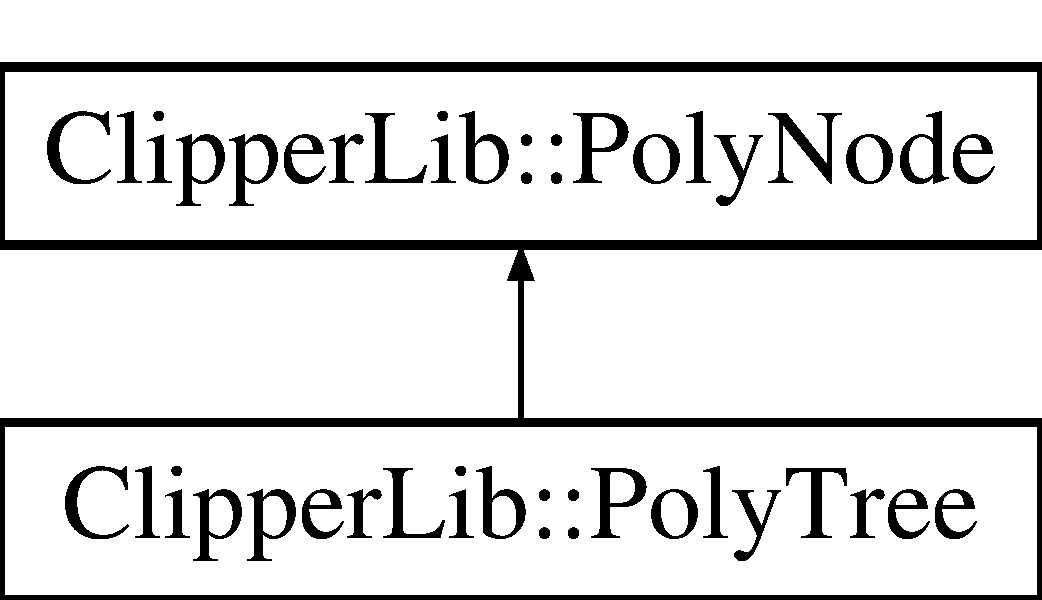
\includegraphics[height=2.000000cm]{classClipperLib_1_1PolyTree}
\end{center}
\end{figure}
\subsection*{Public Member Functions}
\begin{DoxyCompactItemize}
\item 
\hypertarget{classClipperLib_1_1PolyTree_ab678adb646c636e1f7a13e56cdc5bb93}{\hyperlink{classClipperLib_1_1PolyNode}{Poly\-Node} $\ast$ {\bfseries Get\-First} () const }\label{classClipperLib_1_1PolyTree_ab678adb646c636e1f7a13e56cdc5bb93}

\item 
\hypertarget{classClipperLib_1_1PolyTree_a8620ea631d478b3c43274ac084902ec4}{void {\bfseries Clear} ()}\label{classClipperLib_1_1PolyTree_a8620ea631d478b3c43274ac084902ec4}

\item 
\hypertarget{classClipperLib_1_1PolyTree_a28951d9ee7046c57388c7ddcbb3dcb6d}{int {\bfseries Total} () const }\label{classClipperLib_1_1PolyTree_a28951d9ee7046c57388c7ddcbb3dcb6d}

\end{DoxyCompactItemize}
\subsection*{Friends}
\begin{DoxyCompactItemize}
\item 
\hypertarget{classClipperLib_1_1PolyTree_a4d39a09ecdddeeb85930dd4554a54b3c}{class {\bfseries Clipper}}\label{classClipperLib_1_1PolyTree_a4d39a09ecdddeeb85930dd4554a54b3c}

\end{DoxyCompactItemize}
\subsection*{Additional Inherited Members}


The documentation for this class was generated from the following files\-:\begin{DoxyCompactItemize}
\item 
model/clipper/clipper.\-hpp\item 
model/clipper/clipper.\-cpp\end{DoxyCompactItemize}

\hypertarget{classRegion}{\section{Region Class Reference}
\label{classRegion}\index{Region@{Region}}
}
\subsection*{Public Member Functions}
\begin{DoxyCompactItemize}
\item 
\hypertarget{classRegion_a41ba18a2fa719627ef1933d80876f622}{{\bfseries Region} (std\-::vector$<$ \hyperlink{structStochasticEvent}{Stochastic\-Event} $\ast$ $>$ $\ast$event\-List, \hyperlink{classSegment}{Segment} $\ast$lower\-Boundry)}\label{classRegion_a41ba18a2fa719627ef1933d80876f622}

\item 
\hypertarget{classRegion_a4b32e470e65d95d557129accb8cc5dd5}{void {\bfseries print} (std\-::ostream \&out)}\label{classRegion_a4b32e470e65d95d557129accb8cc5dd5}

\item 
\hypertarget{classRegion_a2d113c4b0cb61ceb1a469d1a8ecfbd1d}{bool {\bfseries intersect} (\hyperlink{classSegment}{Segment} \&s, \hyperlink{structPoint}{Point} \&p1, \hyperlink{structPoint}{Point} \&p2)}\label{classRegion_a2d113c4b0cb61ceb1a469d1a8ecfbd1d}

\end{DoxyCompactItemize}
\subsection*{Public Attributes}
\begin{DoxyCompactItemize}
\item 
\hypertarget{classRegion_a28c4bbed633b1e0795b75c765881152e}{std\-::vector$<$ \hyperlink{structStochasticEvent}{Stochastic\-Event} $\ast$ $>$ $\ast$ {\bfseries event\-Segments}}\label{classRegion_a28c4bbed633b1e0795b75c765881152e}

\item 
\hypertarget{classRegion_aec7eda0e18a1cc45b181e37002b43aa8}{\hyperlink{classSegment}{Segment} $\ast$ {\bfseries lower\-Boundry}}\label{classRegion_aec7eda0e18a1cc45b181e37002b43aa8}

\item 
\hypertarget{classRegion_ab67af47f2e4b0c139977abcfc5768750}{\hyperlink{classSegment}{Segment} $\ast$ {\bfseries left\-Boundry}}\label{classRegion_ab67af47f2e4b0c139977abcfc5768750}

\item 
\hypertarget{classRegion_a281bdea20d56af521f274ddd870aac9a}{\hyperlink{classSegment}{Segment} $\ast$ {\bfseries right\-Boundry}}\label{classRegion_a281bdea20d56af521f274ddd870aac9a}

\item 
double \hyperlink{classRegion_af080e4f60bc8a0231ee52d96f69f40e3}{time\-Bias}
\item 
\hyperlink{structMarking}{Marking} $\ast$ \hyperlink{classRegion_aed4910285f30a87eefaf58fd2c96c4e6}{marking}
\end{DoxyCompactItemize}


\subsection{Member Data Documentation}
\hypertarget{classRegion_aed4910285f30a87eefaf58fd2c96c4e6}{\index{Region@{Region}!marking@{marking}}
\index{marking@{marking}!Region@{Region}}
\subsubsection[{marking}]{\setlength{\rightskip}{0pt plus 5cm}{\bf Marking}$\ast$ Region\-::marking}}\label{classRegion_aed4910285f30a87eefaf58fd2c96c4e6}
This marking indicates the marking exactly after the happening of the event which caused us entering this region. so in order to finding of places marking an advancement according to the specified time is needed. \hypertarget{classRegion_af080e4f60bc8a0231ee52d96f69f40e3}{\index{Region@{Region}!time\-Bias@{time\-Bias}}
\index{time\-Bias@{time\-Bias}!Region@{Region}}
\subsubsection[{time\-Bias}]{\setlength{\rightskip}{0pt plus 5cm}double Region\-::time\-Bias}}\label{classRegion_af080e4f60bc8a0231ee52d96f69f40e3}
Each region should have a time bias. which means this is belong to which segment of main stochastic and determinestic line. 

The documentation for this class was generated from the following files\-:\begin{DoxyCompactItemize}
\item 
model/old/Region.\-h\item 
model/old/Region.\-cpp\end{DoxyCompactItemize}

\hypertarget{structClipperLib_1_1Scanbeam}{\section{Clipper\-Lib\-:\-:Scanbeam Struct Reference}
\label{structClipperLib_1_1Scanbeam}\index{Clipper\-Lib\-::\-Scanbeam@{Clipper\-Lib\-::\-Scanbeam}}
}
\subsection*{Public Attributes}
\begin{DoxyCompactItemize}
\item 
\hypertarget{structClipperLib_1_1Scanbeam_a71e4ab9957d1039c6d6666b92236fb71}{long64 {\bfseries Y}}\label{structClipperLib_1_1Scanbeam_a71e4ab9957d1039c6d6666b92236fb71}

\item 
\hypertarget{structClipperLib_1_1Scanbeam_a7e77b169ceff6cd0e079dd0e0b5760e8}{\hyperlink{structClipperLib_1_1Scanbeam}{Scanbeam} $\ast$ {\bfseries next}}\label{structClipperLib_1_1Scanbeam_a7e77b169ceff6cd0e079dd0e0b5760e8}

\end{DoxyCompactItemize}


The documentation for this struct was generated from the following file\-:\begin{DoxyCompactItemize}
\item 
model/clipper/clipper.\-hpp\end{DoxyCompactItemize}

\hypertarget{classSegment}{\section{Segment Class Reference}
\label{classSegment}\index{Segment@{Segment}}
}
Inheritance diagram for Segment\-:\begin{figure}[H]
\begin{center}
\leavevmode
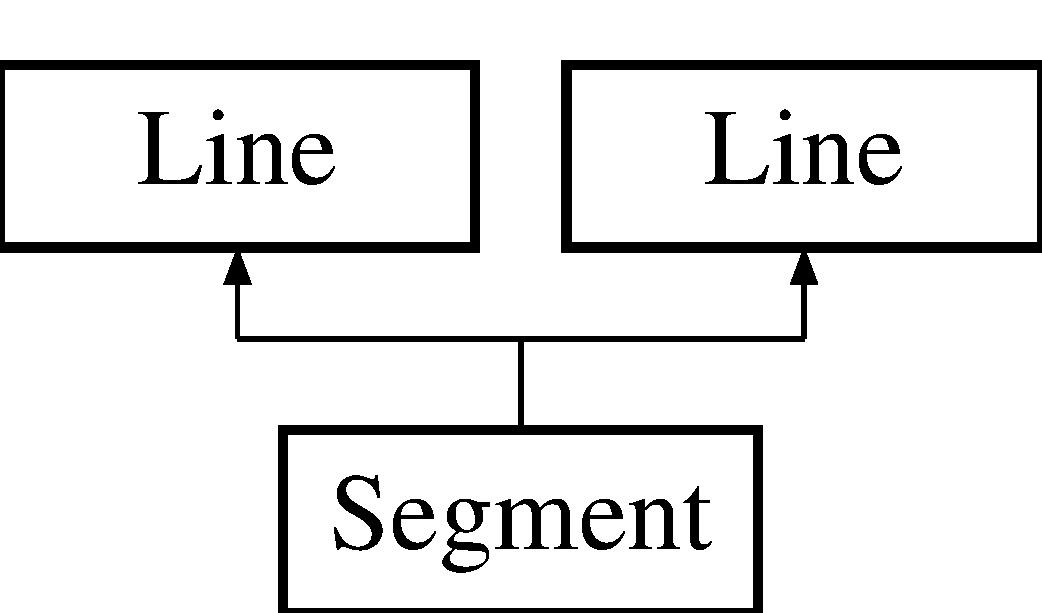
\includegraphics[height=2.000000cm]{classSegment}
\end{center}
\end{figure}
\subsection*{Public Member Functions}
\begin{DoxyCompactItemize}
\item 
\hypertarget{classSegment_ad0e5c8d754ce5a75481cfc7f219c0e89}{{\bfseries Segment} (\hyperlink{structPoint}{Point} \&p1, \hyperlink{structPoint}{Point} \&p2)}\label{classSegment_ad0e5c8d754ce5a75481cfc7f219c0e89}

\item 
\hypertarget{classSegment_aaccb675d9d27369adc8c43cba7b4ca30}{{\bfseries Segment} (double a, double b, \hyperlink{structPoint}{Point} \&p1, \hyperlink{structPoint}{Point} \&p2)}\label{classSegment_aaccb675d9d27369adc8c43cba7b4ca30}

\item 
\hypertarget{classSegment_a3bd6adc6bdf33075f6bdfa0531af2ef0}{{\bfseries Segment} (double a, double b, double start, double end)}\label{classSegment_a3bd6adc6bdf33075f6bdfa0531af2ef0}

\item 
\hypertarget{classSegment_a615337a1fad34f28e0c2b23e40c18521}{{\bfseries Segment} (\hyperlink{classLine}{Line} \&line, double start, double end)}\label{classSegment_a615337a1fad34f28e0c2b23e40c18521}

\item 
\hypertarget{classSegment_a657326272bf487b464c1ccada4f610a7}{\hyperlink{classSegment}{Segment} \& {\bfseries operator=} (const \hyperlink{classSegment}{Segment} \&s)}\label{classSegment_a657326272bf487b464c1ccada4f610a7}

\item 
\hypertarget{classSegment_a105101551a17e1eeaea3a60382c32d99}{bool {\bfseries is\-Up} (\hyperlink{structPoint}{Point} \&p)}\label{classSegment_a105101551a17e1eeaea3a60382c32d99}

\item 
\hypertarget{classSegment_a1da058c85124d8155e5542ece5ed7265}{bool {\bfseries intersect} (\hyperlink{classSegment}{Segment} \&s, \hyperlink{structPoint}{Point} \&int\-Point)}\label{classSegment_a1da058c85124d8155e5542ece5ed7265}

\item 
\hypertarget{classSegment_a1cadab8806d3846eb594fabfcbe48ebe}{Intersection\-Status {\bfseries intersect2} (\hyperlink{classSegment}{Segment} \&s, \hyperlink{structPoint}{Point} \&int\-Point)}\label{classSegment_a1cadab8806d3846eb594fabfcbe48ebe}

\item 
\hypertarget{classSegment_a1d6a246b4cc993eccabd8841b3e5b411}{bool {\bfseries intersect} (\hyperlink{classLine}{Line} \&l, \hyperlink{structPoint}{Point} \&int\-Point)}\label{classSegment_a1d6a246b4cc993eccabd8841b3e5b411}

\item 
\hypertarget{classSegment_a1eaf93a45513f8ba55ae6e59567bbbf5}{void {\bfseries print} ()}\label{classSegment_a1eaf93a45513f8ba55ae6e59567bbbf5}

\item 
\hypertarget{classSegment_ad0e5c8d754ce5a75481cfc7f219c0e89}{{\bfseries Segment} (\hyperlink{structPoint}{Point} \&p1, \hyperlink{structPoint}{Point} \&p2)}\label{classSegment_ad0e5c8d754ce5a75481cfc7f219c0e89}

\item 
\hypertarget{classSegment_aaccb675d9d27369adc8c43cba7b4ca30}{{\bfseries Segment} (double a, double b, \hyperlink{structPoint}{Point} \&p1, \hyperlink{structPoint}{Point} \&p2)}\label{classSegment_aaccb675d9d27369adc8c43cba7b4ca30}

\item 
\hypertarget{classSegment_a3bd6adc6bdf33075f6bdfa0531af2ef0}{{\bfseries Segment} (double a, double b, double start, double end)}\label{classSegment_a3bd6adc6bdf33075f6bdfa0531af2ef0}

\item 
\hypertarget{classSegment_a615337a1fad34f28e0c2b23e40c18521}{{\bfseries Segment} (\hyperlink{classLine}{Line} \&line, double start, double end)}\label{classSegment_a615337a1fad34f28e0c2b23e40c18521}

\item 
\hypertarget{classSegment_aaa84ef4ab376f6668573696a129c547b}{\hyperlink{classSegment}{Segment} \& {\bfseries operator=} (const \hyperlink{classSegment}{Segment} \&s)}\label{classSegment_aaa84ef4ab376f6668573696a129c547b}

\item 
\hypertarget{classSegment_a105101551a17e1eeaea3a60382c32d99}{bool {\bfseries is\-Up} (\hyperlink{structPoint}{Point} \&p)}\label{classSegment_a105101551a17e1eeaea3a60382c32d99}

\item 
\hypertarget{classSegment_a1da058c85124d8155e5542ece5ed7265}{bool {\bfseries intersect} (\hyperlink{classSegment}{Segment} \&s, \hyperlink{structPoint}{Point} \&int\-Point)}\label{classSegment_a1da058c85124d8155e5542ece5ed7265}

\end{DoxyCompactItemize}
\subsection*{Public Attributes}
\begin{DoxyCompactItemize}
\item 
\hypertarget{classSegment_a66dff1645946cc87157a0cbd6d8b23f3}{\hyperlink{structPoint}{Point} {\bfseries p1}}\label{classSegment_a66dff1645946cc87157a0cbd6d8b23f3}

\item 
\hypertarget{classSegment_a9c1f3b8369daf27f3b809cc048f1354f}{\hyperlink{structPoint}{Point} {\bfseries p2}}\label{classSegment_a9c1f3b8369daf27f3b809cc048f1354f}

\end{DoxyCompactItemize}


The documentation for this class was generated from the following files\-:\begin{DoxyCompactItemize}
\item 
model/Line.\-h\item 
model/old/Line.\-h\item 
model/Line.\-cpp\item 
model/old/Line.\-cpp\end{DoxyCompactItemize}

\hypertarget{structState__tag}{\section{State\-\_\-tag Struct Reference}
\label{structState__tag}\index{State\-\_\-tag@{State\-\_\-tag}}
}
\subsection*{Public Attributes}
\begin{DoxyCompactItemize}
\item 
\hypertarget{structState__tag_acc55b277afea86edb39e342931d55dde}{\hyperlink{structMarking}{Marking} $\ast$ {\bfseries M}}\label{structState__tag_acc55b277afea86edb39e342931d55dde}

\item 
\hypertarget{structState__tag_a84d04fbe9a860b99508c3562196dd2f7}{double {\bfseries t0}}\label{structState__tag_a84d04fbe9a860b99508c3562196dd2f7}

\item 
\hypertarget{structState__tag_a11d4f5efa54a1519a0c776cb13fa00f6}{double {\bfseries t1}}\label{structState__tag_a11d4f5efa54a1519a0c776cb13fa00f6}

\item 
\hypertarget{structState__tag_aa2a39da2fb489f889c232fd80a9086b2}{double {\bfseries left\-Int}}\label{structState__tag_aa2a39da2fb489f889c232fd80a9086b2}

\item 
\hypertarget{structState__tag_a3a445d4bcb2c518a6122084f6c114e3e}{double {\bfseries right\-Int}}\label{structState__tag_a3a445d4bcb2c518a6122084f6c114e3e}

\item 
\hypertarget{structState__tag_a784999f0cd357dd7b4c49047465346f7}{int {\bfseries state\-I\-D}}\label{structState__tag_a784999f0cd357dd7b4c49047465346f7}

\item 
\hypertarget{structState__tag_a57478cd95be2c5f4086af0f2e3a3ddfb}{struct \hyperlink{structState__tag}{State\-\_\-tag} $\ast$ {\bfseries next}}\label{structState__tag_a57478cd95be2c5f4086af0f2e3a3ddfb}

\item 
\hypertarget{structState__tag_a5fae5fbcede2d6499d720a76d3f30edd}{struct \hyperlink{structStateTimeAlt__tag}{State\-Time\-Alt\-\_\-tag} $\ast$ {\bfseries next\-State\-List}}\label{structState__tag_a5fae5fbcede2d6499d720a76d3f30edd}

\end{DoxyCompactItemize}


The documentation for this struct was generated from the following files\-:\begin{DoxyCompactItemize}
\item 
model/D\-F\-P\-N2.\-h\item 
model/old/D\-F\-P\-N2.\-h\end{DoxyCompactItemize}

\hypertarget{structStateProbAlt__tag}{\section{State\-Prob\-Alt\-\_\-tag Struct Reference}
\label{structStateProbAlt__tag}\index{State\-Prob\-Alt\-\_\-tag@{State\-Prob\-Alt\-\_\-tag}}
}
\subsection*{Public Attributes}
\begin{DoxyCompactItemize}
\item 
\hypertarget{structStateProbAlt__tag_a2704ecaab5066c9c05586d3ac8febbcc}{double {\bfseries p}}\label{structStateProbAlt__tag_a2704ecaab5066c9c05586d3ac8febbcc}

\item 
\hypertarget{structStateProbAlt__tag_ad448a49570b70caa77da8676c252694b}{\hyperlink{structState__tag}{State} $\ast$ {\bfseries S}}\label{structStateProbAlt__tag_ad448a49570b70caa77da8676c252694b}

\item 
\hypertarget{structStateProbAlt__tag_afbcff4f2be2857039029328b229ec1ea}{struct \hyperlink{structStateProbAlt__tag}{State\-Prob\-Alt\-\_\-tag} $\ast$ {\bfseries next}}\label{structStateProbAlt__tag_afbcff4f2be2857039029328b229ec1ea}

\end{DoxyCompactItemize}


The documentation for this struct was generated from the following files\-:\begin{DoxyCompactItemize}
\item 
model/D\-F\-P\-N2.\-h\item 
model/old/D\-F\-P\-N2.\-h\end{DoxyCompactItemize}

\hypertarget{structStateTimeAlt__tag}{\section{State\-Time\-Alt\-\_\-tag Struct Reference}
\label{structStateTimeAlt__tag}\index{State\-Time\-Alt\-\_\-tag@{State\-Time\-Alt\-\_\-tag}}
}
\subsection*{Public Attributes}
\begin{DoxyCompactItemize}
\item 
\hypertarget{structStateTimeAlt__tag_afabf01ad4269fb670274bd948b504ecb}{\hyperlink{structStateProbAlt__tag}{State\-Prob\-Alt} $\ast$ {\bfseries sa}}\label{structStateTimeAlt__tag_afabf01ad4269fb670274bd948b504ecb}

\item 
\hypertarget{structStateTimeAlt__tag_a39cdb5d8628f31980280f1f7c3ead97e}{double {\bfseries left\-Int}}\label{structStateTimeAlt__tag_a39cdb5d8628f31980280f1f7c3ead97e}

\item 
\hypertarget{structStateTimeAlt__tag_a9f2fa05a0dd6c3c17a34da6fb225c4d3}{double {\bfseries right\-Int}}\label{structStateTimeAlt__tag_a9f2fa05a0dd6c3c17a34da6fb225c4d3}

\item 
\hypertarget{structStateTimeAlt__tag_aac6d881131ab8cc209a37f92442631a2}{struct \hyperlink{structStateTimeAlt__tag}{State\-Time\-Alt\-\_\-tag} $\ast$ {\bfseries next}}\label{structStateTimeAlt__tag_aac6d881131ab8cc209a37f92442631a2}

\end{DoxyCompactItemize}


The documentation for this struct was generated from the following files\-:\begin{DoxyCompactItemize}
\item 
model/D\-F\-P\-N2.\-h\item 
model/old/D\-F\-P\-N2.\-h\end{DoxyCompactItemize}

\hypertarget{classSTDRegion}{\section{S\-T\-D\-Region Class Reference}
\label{classSTDRegion}\index{S\-T\-D\-Region@{S\-T\-D\-Region}}
}
\subsection*{Public Member Functions}
\begin{DoxyCompactItemize}
\item 
\hypertarget{classSTDRegion_a52a3824cb008328519128c2511d3043e}{{\bfseries S\-T\-D\-Region} (std\-::vector$<$ \hyperlink{structStochasticEvent}{Stochastic\-Event} $\ast$ $>$ $\ast$event\-List, \hyperlink{classSegment}{Segment} $\ast$lower\-Boundry)}\label{classSTDRegion_a52a3824cb008328519128c2511d3043e}

\item 
\hypertarget{classSTDRegion_a23a481692098bea54e19f26f6551ab50}{void {\bfseries print} (std\-::ostream \&out)}\label{classSTDRegion_a23a481692098bea54e19f26f6551ab50}

\item 
\hypertarget{classSTDRegion_abb64369d5a5fa5b71231c827066111df}{bool {\bfseries intersect} (\hyperlink{classSegment}{Segment} \&s, \hyperlink{structPoint}{Point} \&p1, \hyperlink{structPoint}{Point} \&p2)}\label{classSTDRegion_abb64369d5a5fa5b71231c827066111df}

\item 
\hypertarget{classSTDRegion_ad45677a054f77585b7087be951630724}{bool {\bfseries intersect} (\hyperlink{classLine}{Line} \&s, \hyperlink{structPoint}{Point} \&p1, \hyperlink{structPoint}{Point} \&p2)}\label{classSTDRegion_ad45677a054f77585b7087be951630724}

\end{DoxyCompactItemize}
\subsection*{Public Attributes}
\begin{DoxyCompactItemize}
\item 
\hypertarget{classSTDRegion_ad665c33c075285e3f6c44db0fc2b2408}{std\-::vector$<$ \hyperlink{structStochasticEvent}{Stochastic\-Event} $\ast$ $>$ $\ast$ {\bfseries event\-Segments}}\label{classSTDRegion_ad665c33c075285e3f6c44db0fc2b2408}

\item 
\hypertarget{classSTDRegion_ad30192b606376da2a13c8a6d44d38a62}{std\-::vector$<$ \hyperlink{classSTDRegion}{S\-T\-D\-Region} $\ast$ $>$ $\ast$ {\bfseries successors}}\label{classSTDRegion_ad30192b606376da2a13c8a6d44d38a62}

\item 
\hypertarget{classSTDRegion_a5699bcbca000b47f0f35d1d2a954482d}{\hyperlink{classSegment}{Segment} $\ast$ {\bfseries lower\-Boundry}}\label{classSTDRegion_a5699bcbca000b47f0f35d1d2a954482d}

\item 
\hypertarget{classSTDRegion_a69d0da9f23e4dd8f79b2cb3ba40e6283}{\hyperlink{classSegment}{Segment} $\ast$ {\bfseries left\-Boundry}}\label{classSTDRegion_a69d0da9f23e4dd8f79b2cb3ba40e6283}

\item 
\hypertarget{classSTDRegion_a10de10f63d9fbd07fe057cd71d91d3c0}{\hyperlink{classSegment}{Segment} $\ast$ {\bfseries right\-Boundry}}\label{classSTDRegion_a10de10f63d9fbd07fe057cd71d91d3c0}

\item 
double \hyperlink{classSTDRegion_a66f6dbac4fc0f9f2b08ac7929ef41295}{time\-Bias}
\item 
\hyperlink{structMarking}{Marking} $\ast$ \hyperlink{classSTDRegion_ad5384bd954f03e3bafaf5bb913ca0485}{marking}
\end{DoxyCompactItemize}


\subsection{Member Data Documentation}
\hypertarget{classSTDRegion_ad5384bd954f03e3bafaf5bb913ca0485}{\index{S\-T\-D\-Region@{S\-T\-D\-Region}!marking@{marking}}
\index{marking@{marking}!STDRegion@{S\-T\-D\-Region}}
\subsubsection[{marking}]{\setlength{\rightskip}{0pt plus 5cm}{\bf Marking}$\ast$ S\-T\-D\-Region\-::marking}}\label{classSTDRegion_ad5384bd954f03e3bafaf5bb913ca0485}
This marking indicates the marking exactly after the happening of the event which caused us entering this region. so in order to finding of places marking an advancement according to the specified time is needed. \hypertarget{classSTDRegion_a66f6dbac4fc0f9f2b08ac7929ef41295}{\index{S\-T\-D\-Region@{S\-T\-D\-Region}!time\-Bias@{time\-Bias}}
\index{time\-Bias@{time\-Bias}!STDRegion@{S\-T\-D\-Region}}
\subsubsection[{time\-Bias}]{\setlength{\rightskip}{0pt plus 5cm}double S\-T\-D\-Region\-::time\-Bias}}\label{classSTDRegion_a66f6dbac4fc0f9f2b08ac7929ef41295}
Each region should have a time bias. which means this is belong to which segment of main stochastic and determinestic line. 

The documentation for this class was generated from the following files\-:\begin{DoxyCompactItemize}
\item 
model/S\-T\-D\-Region.\-h\item 
model/S\-T\-D\-Region.\-cpp\end{DoxyCompactItemize}

\hypertarget{structStochasticEvent}{\section{Stochastic\-Event Struct Reference}
\label{structStochasticEvent}\index{Stochastic\-Event@{Stochastic\-Event}}
}


{\ttfamily \#include $<$Event.\-h$>$}

\subsection*{Public Member Functions}
\begin{DoxyCompactItemize}
\item 
\hypertarget{structStochasticEvent_a6e3ed7abc6f78772300a5b94d64638c8}{{\bfseries Stochastic\-Event} (\hyperlink{classSegment}{Segment} $\ast$line, Event\-Type type)}\label{structStochasticEvent_a6e3ed7abc6f78772300a5b94d64638c8}

\item 
\hypertarget{structStochasticEvent_a37f3e2bc477fa20547b21876551450ca}{{\bfseries Stochastic\-Event} (\hyperlink{structStochasticEvent}{Stochastic\-Event} $\ast$se)}\label{structStochasticEvent_a37f3e2bc477fa20547b21876551450ca}

\item 
\hypertarget{structStochasticEvent_a6e3ed7abc6f78772300a5b94d64638c8}{{\bfseries Stochastic\-Event} (\hyperlink{classSegment}{Segment} $\ast$line, Event\-Type type)}\label{structStochasticEvent_a6e3ed7abc6f78772300a5b94d64638c8}

\item 
\hypertarget{structStochasticEvent_a37f3e2bc477fa20547b21876551450ca}{{\bfseries Stochastic\-Event} (\hyperlink{structStochasticEvent}{Stochastic\-Event} $\ast$se)}\label{structStochasticEvent_a37f3e2bc477fa20547b21876551450ca}

\end{DoxyCompactItemize}
\subsection*{Static Public Member Functions}
\begin{DoxyCompactItemize}
\item 
\hypertarget{structStochasticEvent_a3fee00f7e0b02f6fa83191c903f051a8}{static bool {\bfseries greater\-Slope\-First} (\hyperlink{structStochasticEvent}{Stochastic\-Event} $\ast$e1, \hyperlink{structStochasticEvent}{Stochastic\-Event} $\ast$e2)}\label{structStochasticEvent_a3fee00f7e0b02f6fa83191c903f051a8}

\item 
\hypertarget{structStochasticEvent_a3fee00f7e0b02f6fa83191c903f051a8}{static bool {\bfseries greater\-Slope\-First} (\hyperlink{structStochasticEvent}{Stochastic\-Event} $\ast$e1, \hyperlink{structStochasticEvent}{Stochastic\-Event} $\ast$e2)}\label{structStochasticEvent_a3fee00f7e0b02f6fa83191c903f051a8}

\end{DoxyCompactItemize}
\subsection*{Public Attributes}
\begin{DoxyCompactItemize}
\item 
\hyperlink{classSegment}{Segment} $\ast$ \hyperlink{structStochasticEvent_a39fc3833721f4066c15044e6772a5435}{time\-Segment}
\item 
\hypertarget{structStochasticEvent_a690adfab90bc2fe8652acfa56ac97f5c}{Event\-Type {\bfseries event\-Type}}\label{structStochasticEvent_a690adfab90bc2fe8652acfa56ac97f5c}

\item 
int \hyperlink{structStochasticEvent_a359f6c7f5e9d624744e35fb187adcc73}{id}
\item 
\hyperlink{structMarking}{Marking} $\ast$ \hyperlink{structStochasticEvent_a3179b1980d441007158d7a9c77b8ca1d}{pre\-Region\-Marking}
\item 
\hypertarget{structStochasticEvent_a643f0efa415d0d4a9bf435c9b78fa8df}{\hyperlink{classSTDRegion}{S\-T\-D\-Region} $\ast$ {\bfseries pre\-Region}}\label{structStochasticEvent_a643f0efa415d0d4a9bf435c9b78fa8df}

\item 
\hypertarget{structStochasticEvent_a34eef0f58d7388aae730fc042311826c}{\hyperlink{structDtrmEvent}{Dtrm\-Event} $\ast$ {\bfseries pre\-Dtrm\-Event}}\label{structStochasticEvent_a34eef0f58d7388aae730fc042311826c}

\item 
\hyperlink{structMarking}{Marking} $\ast$ \hyperlink{structStochasticEvent_a9c694991cdb06b9499b9c4295af4d98b}{post\-Region\-Marking}
\end{DoxyCompactItemize}


\subsection{Detailed Description}
Stochastic Event. sd 

\subsection{Member Data Documentation}
\hypertarget{structStochasticEvent_a359f6c7f5e9d624744e35fb187adcc73}{\index{Stochastic\-Event@{Stochastic\-Event}!id@{id}}
\index{id@{id}!StochasticEvent@{Stochastic\-Event}}
\subsubsection[{id}]{\setlength{\rightskip}{0pt plus 5cm}int Stochastic\-Event\-::id}}\label{structStochasticEvent_a359f6c7f5e9d624744e35fb187adcc73}
\hyperlink{structTransition}{Transition} or place I\-D; \hypertarget{structStochasticEvent_a9c694991cdb06b9499b9c4295af4d98b}{\index{Stochastic\-Event@{Stochastic\-Event}!post\-Region\-Marking@{post\-Region\-Marking}}
\index{post\-Region\-Marking@{post\-Region\-Marking}!StochasticEvent@{Stochastic\-Event}}
\subsubsection[{post\-Region\-Marking}]{\setlength{\rightskip}{0pt plus 5cm}{\bf Marking} $\ast$ Stochastic\-Event\-::post\-Region\-Marking}}\label{structStochasticEvent_a9c694991cdb06b9499b9c4295af4d98b}
marking of region before this event happening. \hypertarget{structStochasticEvent_a3179b1980d441007158d7a9c77b8ca1d}{\index{Stochastic\-Event@{Stochastic\-Event}!pre\-Region\-Marking@{pre\-Region\-Marking}}
\index{pre\-Region\-Marking@{pre\-Region\-Marking}!StochasticEvent@{Stochastic\-Event}}
\subsubsection[{pre\-Region\-Marking}]{\setlength{\rightskip}{0pt plus 5cm}{\bf Marking} $\ast$ Stochastic\-Event\-::pre\-Region\-Marking}}\label{structStochasticEvent_a3179b1980d441007158d7a9c77b8ca1d}
marking of region before this event happening. \hypertarget{structStochasticEvent_a39fc3833721f4066c15044e6772a5435}{\index{Stochastic\-Event@{Stochastic\-Event}!time\-Segment@{time\-Segment}}
\index{time\-Segment@{time\-Segment}!StochasticEvent@{Stochastic\-Event}}
\subsubsection[{time\-Segment}]{\setlength{\rightskip}{0pt plus 5cm}{\bf Segment} $\ast$ Stochastic\-Event\-::time\-Segment}}\label{structStochasticEvent_a39fc3833721f4066c15044e6772a5435}
Describes the equation and the validity s-\/interval of next potential event, dependent on $ s $. 

The documentation for this struct was generated from the following files\-:\begin{DoxyCompactItemize}
\item 
model/Event.\-h\item 
model/old/Event.\-h\end{DoxyCompactItemize}

\hypertarget{structClipperLib_1_1TEdge}{\section{Clipper\-Lib\-:\-:T\-Edge Struct Reference}
\label{structClipperLib_1_1TEdge}\index{Clipper\-Lib\-::\-T\-Edge@{Clipper\-Lib\-::\-T\-Edge}}
}
\subsection*{Public Attributes}
\begin{DoxyCompactItemize}
\item 
\hypertarget{structClipperLib_1_1TEdge_a42d3306a851df6869a85f68495a1c4a3}{long64 {\bfseries xbot}}\label{structClipperLib_1_1TEdge_a42d3306a851df6869a85f68495a1c4a3}

\item 
\hypertarget{structClipperLib_1_1TEdge_a5cca9ccc325b346dc2a25001c4291f2a}{long64 {\bfseries ybot}}\label{structClipperLib_1_1TEdge_a5cca9ccc325b346dc2a25001c4291f2a}

\item 
\hypertarget{structClipperLib_1_1TEdge_a26717c33477dbe350518cd0819a9e3c6}{long64 {\bfseries xcurr}}\label{structClipperLib_1_1TEdge_a26717c33477dbe350518cd0819a9e3c6}

\item 
\hypertarget{structClipperLib_1_1TEdge_a075c45d9ae5c1d2d0a22a4778c2f7c74}{long64 {\bfseries ycurr}}\label{structClipperLib_1_1TEdge_a075c45d9ae5c1d2d0a22a4778c2f7c74}

\item 
\hypertarget{structClipperLib_1_1TEdge_ad171f585c0d88630f35fc87706ae1fde}{long64 {\bfseries xtop}}\label{structClipperLib_1_1TEdge_ad171f585c0d88630f35fc87706ae1fde}

\item 
\hypertarget{structClipperLib_1_1TEdge_a56b854b6224c1f0fc7903d5448229a3a}{long64 {\bfseries ytop}}\label{structClipperLib_1_1TEdge_a56b854b6224c1f0fc7903d5448229a3a}

\item 
\hypertarget{structClipperLib_1_1TEdge_aab44ea427e3da1631c15e1ff7c913108}{double {\bfseries dx}}\label{structClipperLib_1_1TEdge_aab44ea427e3da1631c15e1ff7c913108}

\item 
\hypertarget{structClipperLib_1_1TEdge_ab27923f96c12e80a3e6c95776333c811}{long64 {\bfseries delta\-X}}\label{structClipperLib_1_1TEdge_ab27923f96c12e80a3e6c95776333c811}

\item 
\hypertarget{structClipperLib_1_1TEdge_a103279aab6bb41f5c0672b9a7b79014b}{long64 {\bfseries delta\-Y}}\label{structClipperLib_1_1TEdge_a103279aab6bb41f5c0672b9a7b79014b}

\item 
\hypertarget{structClipperLib_1_1TEdge_a4ec20b0f419c70c81d57d3e1da27daf6}{long64 {\bfseries tmp\-X}}\label{structClipperLib_1_1TEdge_a4ec20b0f419c70c81d57d3e1da27daf6}

\item 
\hypertarget{structClipperLib_1_1TEdge_abcbfff8dad739351094a02487e59f4e7}{Poly\-Type {\bfseries poly\-Type}}\label{structClipperLib_1_1TEdge_abcbfff8dad739351094a02487e59f4e7}

\item 
\hypertarget{structClipperLib_1_1TEdge_a2024ade454223f57339ab6045d182e55}{Edge\-Side {\bfseries side}}\label{structClipperLib_1_1TEdge_a2024ade454223f57339ab6045d182e55}

\item 
\hypertarget{structClipperLib_1_1TEdge_a2e5b86c66d319f01e32b5d06596e36fb}{int {\bfseries wind\-Delta}}\label{structClipperLib_1_1TEdge_a2e5b86c66d319f01e32b5d06596e36fb}

\item 
\hypertarget{structClipperLib_1_1TEdge_a24e0e2bd7a90676c7a7ad5e2052878ed}{int {\bfseries wind\-Cnt}}\label{structClipperLib_1_1TEdge_a24e0e2bd7a90676c7a7ad5e2052878ed}

\item 
\hypertarget{structClipperLib_1_1TEdge_a803d452baf10e1cd5f5e17f758b298df}{int {\bfseries wind\-Cnt2}}\label{structClipperLib_1_1TEdge_a803d452baf10e1cd5f5e17f758b298df}

\item 
\hypertarget{structClipperLib_1_1TEdge_a63e563de2857398a9c8b0d4904679d84}{int {\bfseries out\-Idx}}\label{structClipperLib_1_1TEdge_a63e563de2857398a9c8b0d4904679d84}

\item 
\hypertarget{structClipperLib_1_1TEdge_a21c3dba96acc90b5bc00ca3db68445f6}{\hyperlink{structClipperLib_1_1TEdge}{T\-Edge} $\ast$ {\bfseries next}}\label{structClipperLib_1_1TEdge_a21c3dba96acc90b5bc00ca3db68445f6}

\item 
\hypertarget{structClipperLib_1_1TEdge_ac81ef1c52f20b36b321d2a9208f97389}{\hyperlink{structClipperLib_1_1TEdge}{T\-Edge} $\ast$ {\bfseries prev}}\label{structClipperLib_1_1TEdge_ac81ef1c52f20b36b321d2a9208f97389}

\item 
\hypertarget{structClipperLib_1_1TEdge_af9f1d12d9a024e0aeb0a5810e66a343d}{\hyperlink{structClipperLib_1_1TEdge}{T\-Edge} $\ast$ {\bfseries next\-In\-L\-M\-L}}\label{structClipperLib_1_1TEdge_af9f1d12d9a024e0aeb0a5810e66a343d}

\item 
\hypertarget{structClipperLib_1_1TEdge_a2e4f5e8ffce918c2d5cf260252a4e811}{\hyperlink{structClipperLib_1_1TEdge}{T\-Edge} $\ast$ {\bfseries next\-In\-A\-E\-L}}\label{structClipperLib_1_1TEdge_a2e4f5e8ffce918c2d5cf260252a4e811}

\item 
\hypertarget{structClipperLib_1_1TEdge_a0da02ede8e83c3a4b27a09ebde1dfcf3}{\hyperlink{structClipperLib_1_1TEdge}{T\-Edge} $\ast$ {\bfseries prev\-In\-A\-E\-L}}\label{structClipperLib_1_1TEdge_a0da02ede8e83c3a4b27a09ebde1dfcf3}

\item 
\hypertarget{structClipperLib_1_1TEdge_aa98ac28e25e2a0bf4001ca9547ea0ae8}{\hyperlink{structClipperLib_1_1TEdge}{T\-Edge} $\ast$ {\bfseries next\-In\-S\-E\-L}}\label{structClipperLib_1_1TEdge_aa98ac28e25e2a0bf4001ca9547ea0ae8}

\item 
\hypertarget{structClipperLib_1_1TEdge_aead630eae0633921989272f74d7d169b}{\hyperlink{structClipperLib_1_1TEdge}{T\-Edge} $\ast$ {\bfseries prev\-In\-S\-E\-L}}\label{structClipperLib_1_1TEdge_aead630eae0633921989272f74d7d169b}

\end{DoxyCompactItemize}


The documentation for this struct was generated from the following file\-:\begin{DoxyCompactItemize}
\item 
model/clipper/clipper.\-hpp\end{DoxyCompactItemize}

\hypertarget{classTimedDiagram}{\section{Timed\-Diagram Class Reference}
\label{classTimedDiagram}\index{Timed\-Diagram@{Timed\-Diagram}}
}
\subsection*{Public Member Functions}
\begin{DoxyCompactItemize}
\item 
\hypertarget{classTimedDiagram_adf699c8fddf11d5357faf2ef29bddd7c}{void {\bfseries set\-Model} (\hyperlink{structModel}{Model} $\ast$model)}\label{classTimedDiagram_adf699c8fddf11d5357faf2ef29bddd7c}

\item 
\hypertarget{classTimedDiagram_a7055f706b0c2444185e8d5d878626523}{void {\bfseries clear} ()}\label{classTimedDiagram_a7055f706b0c2444185e8d5d878626523}

\item 
void \hyperlink{classTimedDiagram_a55bc9188cb14b08bc95dde3778579f90}{generate\-Diagram} (\hyperlink{structMarking}{Marking} $\ast$initial\-Marking)
\item 
void \hyperlink{classTimedDiagram_aed76b48c2a65ee7ea16a393de058e581}{compute\-Next\-Events} (std\-::vector$<$ \hyperlink{structStochasticEvent}{Stochastic\-Event} $\ast$ $>$ $\ast$potential\-Events, \hyperlink{classSegment}{Segment} $\ast$u\-Segment, std\-::vector$<$ \hyperlink{structStochasticEvent}{Stochastic\-Event} $\ast$ $>$ $\ast$next\-Events)
\begin{DoxyCompactList}\small\item\em This function takes the minimum of input event lines set, in the t-\/s frame. It returns the sorted resulting segments. T\-O\-D\-O\-: consider multiple events at the same time. \end{DoxyCompactList}\item 
\hypertarget{classTimedDiagram_a51004d1d8a2ae7d80a089a54ecf93fec}{void {\bfseries Segmentize\-Dtrm\-Region} (\hyperlink{structMarking}{Marking} $\ast$marking)}\label{classTimedDiagram_a51004d1d8a2ae7d80a089a54ecf93fec}

\item 
void \hyperlink{classTimedDiagram_aa8d8af4ac9f2e51d12b6ae23b8c506c1}{segmentize\-Stochastic\-Region} (\hyperlink{structMarking}{Marking} $\ast$marking, \hyperlink{structStochasticEvent}{Stochastic\-Event} $\ast$event\-Line, double time\-Bias)
\item 
double \hyperlink{classTimedDiagram_a45ef38a01bcffd182224747bd2a96041}{cal\-Prob\-At\-Time} (double time, double($\ast$s\-Pdf\-Int)(double), bool($\ast$is\-Prop\-Holds)(\hyperlink{structModel}{Model} $\ast$, \hyperlink{structMarking}{Marking} $\ast$, double t0, double t1, double \&, double \&))
\item 
\hypertarget{classTimedDiagram_aa0eafacca33acf296c5bd1219f12fed8}{int {\bfseries get\-Number\-Of\-Regions} ()}\label{classTimedDiagram_aa0eafacca33acf296c5bd1219f12fed8}

\item 
\hypertarget{classTimedDiagram_adf699c8fddf11d5357faf2ef29bddd7c}{void {\bfseries set\-Model} (\hyperlink{structModel}{Model} $\ast$model)}\label{classTimedDiagram_adf699c8fddf11d5357faf2ef29bddd7c}

\item 
\hypertarget{classTimedDiagram_a7055f706b0c2444185e8d5d878626523}{void {\bfseries clear} ()}\label{classTimedDiagram_a7055f706b0c2444185e8d5d878626523}

\item 
\hypertarget{classTimedDiagram_a55bc9188cb14b08bc95dde3778579f90}{void {\bfseries generate\-Diagram} (\hyperlink{structMarking}{Marking} $\ast$initial\-Marking)}\label{classTimedDiagram_a55bc9188cb14b08bc95dde3778579f90}

\item 
void \hyperlink{classTimedDiagram_aed76b48c2a65ee7ea16a393de058e581}{compute\-Next\-Events} (std\-::vector$<$ \hyperlink{structStochasticEvent}{Stochastic\-Event} $\ast$ $>$ $\ast$potential\-Events, \hyperlink{classSegment}{Segment} $\ast$u\-Segment, std\-::vector$<$ \hyperlink{structStochasticEvent}{Stochastic\-Event} $\ast$ $>$ $\ast$next\-Events)
\begin{DoxyCompactList}\small\item\em This function takes the minimum of input event lines set, in the t-\/s frame. It returns the sorted resulting segments. T\-O\-D\-O\-: consider multiple events at the same time. \end{DoxyCompactList}\item 
\hypertarget{classTimedDiagram_a51004d1d8a2ae7d80a089a54ecf93fec}{void {\bfseries Segmentize\-Dtrm\-Region} (\hyperlink{structMarking}{Marking} $\ast$marking)}\label{classTimedDiagram_a51004d1d8a2ae7d80a089a54ecf93fec}

\item 
void \hyperlink{classTimedDiagram_aa8d8af4ac9f2e51d12b6ae23b8c506c1}{segmentize\-Stochastic\-Region} (\hyperlink{structMarking}{Marking} $\ast$marking, \hyperlink{structStochasticEvent}{Stochastic\-Event} $\ast$event\-Line, double time\-Bias)
\item 
double \hyperlink{classTimedDiagram_a45ef38a01bcffd182224747bd2a96041}{cal\-Prob\-At\-Time} (double time, double($\ast$s\-Pdf\-Int)(double), bool($\ast$is\-Prop\-Holds)(\hyperlink{structModel}{Model} $\ast$, \hyperlink{structMarking}{Marking} $\ast$, double t0, double t1, double \&, double \&))
\item 
\hypertarget{classTimedDiagram_a070d39903157613803111d696f54a7d0}{void {\bfseries save\-Diagram} (std\-::string filename)}\label{classTimedDiagram_a070d39903157613803111d696f54a7d0}

\item 
\hypertarget{classTimedDiagram_a5fadc1d768a55ee74864ee05dc1c7c23}{double {\bfseries get\-Tr\-Enabled\-Time} () const }\label{classTimedDiagram_a5fadc1d768a55ee74864ee05dc1c7c23}

\item 
\hypertarget{classTimedDiagram_aa0eafacca33acf296c5bd1219f12fed8}{int {\bfseries get\-Number\-Of\-Regions} ()}\label{classTimedDiagram_aa0eafacca33acf296c5bd1219f12fed8}

\end{DoxyCompactItemize}
\subsection*{Static Public Member Functions}
\begin{DoxyCompactItemize}
\item 
\hypertarget{classTimedDiagram_a9003646431725e6901bf7eacfd2a3775}{static \hyperlink{classTimedDiagram}{Timed\-Diagram} $\ast$ {\bfseries get\-Instance} ()}\label{classTimedDiagram_a9003646431725e6901bf7eacfd2a3775}

\item 
\hypertarget{classTimedDiagram_a45a59b6448eae518ed352328cd703ee3}{static \hyperlink{classTimedDiagram}{Timed\-Diagram} $\ast$ {\bfseries get\-Instance} ()}\label{classTimedDiagram_a45a59b6448eae518ed352328cd703ee3}

\end{DoxyCompactItemize}
\subsection*{Public Attributes}
\begin{DoxyCompactItemize}
\item 
\hypertarget{classTimedDiagram_ad7f4b0079de06896c5e17f59c4fd9a67}{\hyperlink{structModel}{Model} $\ast$ {\bfseries model}}\label{classTimedDiagram_ad7f4b0079de06896c5e17f59c4fd9a67}

\item 
std\-::vector$<$ \hyperlink{classSTDRegion}{S\-T\-D\-Region} $\ast$ $>$ \hyperlink{classTimedDiagram_a78e0edbe8a03e71f0d229891ef4abe11}{region\-List}
\item 
\hypertarget{classTimedDiagram_a8b56e04641a67753c7a9ef544cab634e}{cv\-::\-Mat {\bfseries debug\-Image}}\label{classTimedDiagram_a8b56e04641a67753c7a9ef544cab634e}

\item 
\hypertarget{classTimedDiagram_ae0fdae2d323f9d062946805d7de78a99}{int {\bfseries scale}}\label{classTimedDiagram_ae0fdae2d323f9d062946805d7de78a99}

\end{DoxyCompactItemize}


\subsection{Member Function Documentation}
\hypertarget{classTimedDiagram_a45ef38a01bcffd182224747bd2a96041}{\index{Timed\-Diagram@{Timed\-Diagram}!cal\-Prob\-At\-Time@{cal\-Prob\-At\-Time}}
\index{cal\-Prob\-At\-Time@{cal\-Prob\-At\-Time}!TimedDiagram@{Timed\-Diagram}}
\subsubsection[{cal\-Prob\-At\-Time}]{\setlength{\rightskip}{0pt plus 5cm}double Timed\-Diagram\-::cal\-Prob\-At\-Time (
\begin{DoxyParamCaption}
\item[{double}]{time, }
\item[{double($\ast$)(double)}]{s\-Pdf\-Int, }
\item[{bool($\ast$)({\bf Model} $\ast$, {\bf Marking} $\ast$, double t0, double t1, double \&, double \&)}]{is\-Prop\-Holds}
\end{DoxyParamCaption}
)}}\label{classTimedDiagram_a45ef38a01bcffd182224747bd2a96041}

\begin{DoxyParams}{Parameters}
{\em time} & The time for which probability calculation is being done. \\
\hline
{\em s\-Pdf\-Int} & Pointer to the integral pdf of s. \\
\hline
{\em is\-Prop\-Holds} & Pointer to the function which determines whether a spesific property for a marking holds. This function returns the interval that the property holds. \\
\hline
\end{DoxyParams}
\begin{DoxyReturn}{Returns}
The probabilty that the given property holds for a given time. 
\end{DoxyReturn}
\hypertarget{classTimedDiagram_a45ef38a01bcffd182224747bd2a96041}{\index{Timed\-Diagram@{Timed\-Diagram}!cal\-Prob\-At\-Time@{cal\-Prob\-At\-Time}}
\index{cal\-Prob\-At\-Time@{cal\-Prob\-At\-Time}!TimedDiagram@{Timed\-Diagram}}
\subsubsection[{cal\-Prob\-At\-Time}]{\setlength{\rightskip}{0pt plus 5cm}double Timed\-Diagram\-::cal\-Prob\-At\-Time (
\begin{DoxyParamCaption}
\item[{double}]{time, }
\item[{double($\ast$)(double)}]{s\-Pdf\-Int, }
\item[{bool($\ast$)({\bf Model} $\ast$, {\bf Marking} $\ast$, double t0, double t1, double \&, double \&)}]{is\-Prop\-Holds}
\end{DoxyParamCaption}
)}}\label{classTimedDiagram_a45ef38a01bcffd182224747bd2a96041}

\begin{DoxyParams}{Parameters}
{\em time} & The time for which probability calculation is being done. \\
\hline
{\em s\-Pdf\-Int} & Pointer to the integral pdf of s. \\
\hline
{\em is\-Prop\-Holds} & Pointer to the function which determines whether a spesific property for a marking holds. This function returns the interval that the property holds. \\
\hline
\end{DoxyParams}
\begin{DoxyReturn}{Returns}
The probabilty that the given property holds for a given time. 
\end{DoxyReturn}
\hypertarget{classTimedDiagram_aed76b48c2a65ee7ea16a393de058e581}{\index{Timed\-Diagram@{Timed\-Diagram}!compute\-Next\-Events@{compute\-Next\-Events}}
\index{compute\-Next\-Events@{compute\-Next\-Events}!TimedDiagram@{Timed\-Diagram}}
\subsubsection[{compute\-Next\-Events}]{\setlength{\rightskip}{0pt plus 5cm}void Timed\-Diagram\-::compute\-Next\-Events (
\begin{DoxyParamCaption}
\item[{std\-::vector$<$ {\bf Stochastic\-Event} $\ast$ $>$ $\ast$}]{potential\-Events, }
\item[{{\bf Segment} $\ast$}]{u\-Segment, }
\item[{std\-::vector$<$ {\bf Stochastic\-Event} $\ast$ $>$ $\ast$}]{next\-Events}
\end{DoxyParamCaption}
)}}\label{classTimedDiagram_aed76b48c2a65ee7ea16a393de058e581}


This function takes the minimum of input event lines set, in the t-\/s frame. It returns the sorted resulting segments. T\-O\-D\-O\-: consider multiple events at the same time. 


\begin{DoxyParams}{Parameters}
{\em potential\-Events} & List of possible next events. \\
\hline
{\em u\-Segment} & underlying segment. \\
\hline
{\em start} & Beginning of working interval. \\
\hline
{\em end} & End of working interval. \\
\hline
{\em next\-Events} & List computed next events, depending on the value of $ s$. \textbackslash{} Have in mind this list is sorted by the value of $ s$. This means that the first element of the list is the one happening by lower value of $ s$ \\
\hline
\end{DoxyParams}
\hypertarget{classTimedDiagram_aed76b48c2a65ee7ea16a393de058e581}{\index{Timed\-Diagram@{Timed\-Diagram}!compute\-Next\-Events@{compute\-Next\-Events}}
\index{compute\-Next\-Events@{compute\-Next\-Events}!TimedDiagram@{Timed\-Diagram}}
\subsubsection[{compute\-Next\-Events}]{\setlength{\rightskip}{0pt plus 5cm}void Timed\-Diagram\-::compute\-Next\-Events (
\begin{DoxyParamCaption}
\item[{std\-::vector$<$ {\bf Stochastic\-Event} $\ast$ $>$ $\ast$}]{potential\-Events, }
\item[{{\bf Segment} $\ast$}]{u\-Segment, }
\item[{std\-::vector$<$ {\bf Stochastic\-Event} $\ast$ $>$ $\ast$}]{next\-Events}
\end{DoxyParamCaption}
)}}\label{classTimedDiagram_aed76b48c2a65ee7ea16a393de058e581}


This function takes the minimum of input event lines set, in the t-\/s frame. It returns the sorted resulting segments. T\-O\-D\-O\-: consider multiple events at the same time. 


\begin{DoxyParams}{Parameters}
{\em potential\-Events} & List of possible next events. \\
\hline
{\em u\-Segment} & underlying segment. \\
\hline
{\em start} & Beginning of working interval. \\
\hline
{\em end} & End of working interval. \\
\hline
{\em next\-Events} & List computed next events, depending on the value of $ s$. \textbackslash{} Have in mind this list is sorted by the value of $ s$. This means that the first element of the list is the one happening by lower value of $ s$ \\
\hline
\end{DoxyParams}
\hypertarget{classTimedDiagram_a55bc9188cb14b08bc95dde3778579f90}{\index{Timed\-Diagram@{Timed\-Diagram}!generate\-Diagram@{generate\-Diagram}}
\index{generate\-Diagram@{generate\-Diagram}!TimedDiagram@{Timed\-Diagram}}
\subsubsection[{generate\-Diagram}]{\setlength{\rightskip}{0pt plus 5cm}void Timed\-Diagram\-::generate\-Diagram (
\begin{DoxyParamCaption}
\item[{{\bf Marking} $\ast$}]{initial\-Marking}
\end{DoxyParamCaption}
)}}\label{classTimedDiagram_a55bc9188cb14b08bc95dde3778579f90}
Generating the stochastic (top of $ t = s $ line) part of diagram.

The reason for (-\/ start\-Point.\-Y) is that we should shift the time to the frame with origin at (start\-Point.\-Y, start\-Point.\-Y). (This is how the algorithm is designed, there are other ways too!!)\hypertarget{classTimedDiagram_aa8d8af4ac9f2e51d12b6ae23b8c506c1}{\index{Timed\-Diagram@{Timed\-Diagram}!segmentize\-Stochastic\-Region@{segmentize\-Stochastic\-Region}}
\index{segmentize\-Stochastic\-Region@{segmentize\-Stochastic\-Region}!TimedDiagram@{Timed\-Diagram}}
\subsubsection[{segmentize\-Stochastic\-Region}]{\setlength{\rightskip}{0pt plus 5cm}void Timed\-Diagram\-::segmentize\-Stochastic\-Region (
\begin{DoxyParamCaption}
\item[{{\bf Marking} $\ast$}]{marking, }
\item[{{\bf Stochastic\-Event} $\ast$}]{event\-Line, }
\item[{double}]{time\-Bias}
\end{DoxyParamCaption}
)}}\label{classTimedDiagram_aa8d8af4ac9f2e51d12b6ae23b8c506c1}

\begin{DoxyParams}{Parameters}
{\em marking} & Current marking of the system. \\
\hline
{\em event\-Line} & This is the equation of the lower boundary of region we wish to segmentize. \textbackslash{} Have in mind that this is a segment so it has the validity interval in itself.\\
\hline
\end{DoxyParams}
Each (potential) region to be segmentized at first consists of starting and ending for 's' (like the previous intervals), and an event line, which specifies the equation for $t$ (the time after which the event has occurred) depending on $s$. This function recursively segmentize such regions, by finding linear equations of all the possible next events. Note 1 \-: It is assumed that this function is called only for the upper part of st-\/diagram (when the general transition is fired.) Note 2 \-: Remember that initial marking for this function to start should be such that general transition is fired. \hypertarget{classTimedDiagram_aa8d8af4ac9f2e51d12b6ae23b8c506c1}{\index{Timed\-Diagram@{Timed\-Diagram}!segmentize\-Stochastic\-Region@{segmentize\-Stochastic\-Region}}
\index{segmentize\-Stochastic\-Region@{segmentize\-Stochastic\-Region}!TimedDiagram@{Timed\-Diagram}}
\subsubsection[{segmentize\-Stochastic\-Region}]{\setlength{\rightskip}{0pt plus 5cm}void Timed\-Diagram\-::segmentize\-Stochastic\-Region (
\begin{DoxyParamCaption}
\item[{{\bf Marking} $\ast$}]{marking, }
\item[{{\bf Stochastic\-Event} $\ast$}]{event\-Line, }
\item[{double}]{time\-Bias}
\end{DoxyParamCaption}
)}}\label{classTimedDiagram_aa8d8af4ac9f2e51d12b6ae23b8c506c1}

\begin{DoxyParams}{Parameters}
{\em marking} & Current marking of the system. \\
\hline
{\em event\-Line} & This is the equation of the lower boundary of region we wish to segmentize. We expect this event to contain its parent region.\textbackslash{} Have in mind that this is a segment so it has the validity interval in itself.\\
\hline
\end{DoxyParams}
Each (potential) region to be segmentized at first consists of starting and ending for 's' (like the previous intervals), and an event line, which specifies the equation for $t$ (the time after which the event has occurred) depending on $s$. This function recursively segmentize such regions, by finding linear equations of all the possible next events. Note 1 \-: It is assumed that this function is called only for the upper part of st-\/diagram (when the general transition is fired.) Note 2 \-: Remember that initial marking for this function to start should be such that general transition is fired. 

\subsection{Member Data Documentation}
\hypertarget{classTimedDiagram_a78e0edbe8a03e71f0d229891ef4abe11}{\index{Timed\-Diagram@{Timed\-Diagram}!region\-List@{region\-List}}
\index{region\-List@{region\-List}!TimedDiagram@{Timed\-Diagram}}
\subsubsection[{region\-List}]{\setlength{\rightskip}{0pt plus 5cm}std\-::vector$<${\bf S\-T\-D\-Region}$\ast$$>$ Timed\-Diagram\-::region\-List}}\label{classTimedDiagram_a78e0edbe8a03e71f0d229891ef4abe11}
This vector contains list of region after firing of general transition, i.\-e. at the top of ts-\/line. 

The documentation for this class was generated from the following files\-:\begin{DoxyCompactItemize}
\item 
model/old/Timed\-Diagram.\-h\item 
model/Timed\-Diagram.\-h\item 
model/old/Timed\-Diagram.\-cpp\item 
model/Timed\-Diagram.\-cpp\end{DoxyCompactItemize}

\hypertarget{structTransition}{\section{Transition Struct Reference}
\label{structTransition}\index{Transition@{Transition}}
}
\subsection*{Public Attributes}
\begin{DoxyCompactItemize}
\item 
\hypertarget{structTransition_a805ae5d009fcac5d7f46fd463470ce07}{int {\bfseries type}}\label{structTransition_a805ae5d009fcac5d7f46fd463470ce07}

\item 
\hypertarget{structTransition_a43474faab866ad2a5cdbd17fbc568312}{char $\ast$ {\bfseries id}}\label{structTransition_a43474faab866ad2a5cdbd17fbc568312}

\item 
\hypertarget{structTransition_ada913a006d7b1fef09d3265de5005f74}{double {\bfseries time}}\label{structTransition_ada913a006d7b1fef09d3265de5005f74}

\item 
\hypertarget{structTransition_ab779916e07d91bc5162b86661e5fc3e2}{double {\bfseries weight}}\label{structTransition_ab779916e07d91bc5162b86661e5fc3e2}

\item 
\hypertarget{structTransition_a78c269a5c47d9c0622c441cd8271ac60}{int {\bfseries priority}}\label{structTransition_a78c269a5c47d9c0622c441cd8271ac60}

\item 
\hypertarget{structTransition_a98ffbaa4092f7ce9f6d30789260e1e6b}{double {\bfseries flow\-Rate}}\label{structTransition_a98ffbaa4092f7ce9f6d30789260e1e6b}

\item 
\hypertarget{structTransition_a75d816d622d2a43ab97de0b5eaf25d37}{char $\ast$ {\bfseries df\-\_\-argument}}\label{structTransition_a75d816d622d2a43ab97de0b5eaf25d37}

\item 
\hypertarget{structTransition_a8e1caa51ca0ef8fa008318ac5d4d0d9c}{int {\bfseries df\-\_\-distr}}\label{structTransition_a8e1caa51ca0ef8fa008318ac5d4d0d9c}

\item 
\hypertarget{structTransition_a2a7a93fbc4bd373198081351db626313}{int {\bfseries input\-List\-Size}}\label{structTransition_a2a7a93fbc4bd373198081351db626313}

\item 
\hypertarget{structTransition_ab4c4ecebe3b1a381fe834a0543e4a81a}{int $\ast$ {\bfseries input\-List}}\label{structTransition_ab4c4ecebe3b1a381fe834a0543e4a81a}

\item 
\hypertarget{structTransition_ac7a21bce5fa13011d32df0a5a83a8279}{int {\bfseries inhib\-List\-Size}}\label{structTransition_ac7a21bce5fa13011d32df0a5a83a8279}

\item 
\hypertarget{structTransition_a7b5491e031e904ab608a2450d2d785e9}{int $\ast$ {\bfseries inhib\-List}}\label{structTransition_a7b5491e031e904ab608a2450d2d785e9}

\item 
\hypertarget{structTransition_ab18bdec22309f4a74e4499f88c94d6f6}{int {\bfseries test\-List\-Size}}\label{structTransition_ab18bdec22309f4a74e4499f88c94d6f6}

\item 
\hypertarget{structTransition_a17f4f93d59ca57cbbba758e0361b9708}{int $\ast$ {\bfseries test\-List}}\label{structTransition_a17f4f93d59ca57cbbba758e0361b9708}

\item 
\hypertarget{structTransition_a5431eaaddb162ecec9af6f4a5a150417}{int {\bfseries output\-List\-Size}}\label{structTransition_a5431eaaddb162ecec9af6f4a5a150417}

\item 
\hypertarget{structTransition_ad38a3bc17b3ef9aecad0cf5df42c9155}{int $\ast$ {\bfseries output\-List}}\label{structTransition_ad38a3bc17b3ef9aecad0cf5df42c9155}

\item 
\hypertarget{structTransition_a890829881d0442a6f258f55bef2a1470}{int {\bfseries id\-In\-Marking}}\label{structTransition_a890829881d0442a6f258f55bef2a1470}

\end{DoxyCompactItemize}


The documentation for this struct was generated from the following files\-:\begin{DoxyCompactItemize}
\item 
model/D\-F\-P\-N2.\-h\item 
model/old/D\-F\-P\-N2.\-h\end{DoxyCompactItemize}

\addcontentsline{toc}{part}{Index}
\printindex
\end{document}
